\documentclass[enabledeprecatedfontcommands,fontsize=12pt,paper=a4,twoside,parskip=half]{scrartcl}

\newcommand{\grad}{\ensuremath{^{\circ}} }
\renewcommand{\strut}{\vrule width 0pt height5mm depth2mm}

\usepackage[utf8]{inputenc}
\usepackage[T1]{fontenc}
\usepackage[final]{pdfpages}
% obere Seitenränder gestalten können
\usepackage{fancyhdr}
\usepackage{moreverb}
% Graphiken als jpg, png etc. einbinden können
\usepackage{graphicx}
\usepackage{stmaryrd}
% Floats Objekte mit [H] festsetzen
\usepackage{float}
% setzt URL's schön mit \url{http://bla.laber.com/~mypage}
\usepackage{url}
% Externe PDF's einbinden können
\usepackage{pdflscape}
% Verweise innerhalb des Dokuments schick mit " ... auf Seite ... "
% automatisch versehen. Dazu \vref{labelname} benutzen
\usepackage[ngerman]{varioref}
\usepackage[ngerman]{babel}
% Bibliographie
\usepackage{bibgerm}
% Tabellen
\usepackage{tabularx}
\usepackage{supertabular}
\usepackage[colorlinks=true, pdfstartview=FitV, linkcolor=blue,
            citecolor=blue, urlcolor=blue, hyperfigures=true,
            pdftex=true]{hyperref}
\usepackage{bookmark}
\usepackage{longtable,booktabs}
\usepackage[autostyle,german=guillemets]{csquotes}
\usepackage{blindtext}
\usepackage{mathptmx}
\usepackage[scaled=.92]{helvet}

%%% nobreakhline für die Longtables %%%

\makeatletter
\def\nobreakhline{%
  \noalign{\ifnum0=`}\fi
    \penalty\@M
    \futurelet\@let@token\LT@@nobreakhline}
\def\LT@@nobreakhline{%
  \ifx\@let@token\hline
    \global\let\@gtempa\@gobble
    \gdef\LT@sep{\penalty\@M\vskip\doublerulesep}% <-- change here
  \else
    \global\let\@gtempa\@empty
    \gdef\LT@sep{\penalty\@M\vskip-\arrayrulewidth}% <-- change here
  \fi
  \ifnum0=`{\fi}%
  \multispan\LT@cols
     \unskip\leaders\hrule\@height\arrayrulewidth\hfill\cr
  \noalign{\LT@sep}%
  \multispan\LT@cols
     \unskip\leaders\hrule\@height\arrayrulewidth\hfill\cr
  \noalign{\penalty\@M}%
  \@gtempa}
\makeatother

\hyphenation{Arbeits-paket}

\usepackage[xindy,
            acronym,
            section=subsubsection,
            toc,
            numberedsection]{glossaries} 

% Damit Latex nicht zu lange Zeilen produziert:
\sloppy
%Uneinheitlicher unterer Seitenrand:
%\raggedbottom

% Seitenränder für Korrekturen verändern
\addtolength{\evensidemargin}{-1cm}
\addtolength{\oddsidemargin}{1cm}

\newcommand{\emaillink}[1]{\href{mailto:#1}{#1}}

\usepackage[
backend=biber,
% style=apa 
style=ieee
]{biblatex}
% \DeclareLanguageMapping{ngerman}{ngerman-apa}

\usepackage{booktabs}

\addbibresource{bibo.bib}

%%% Definitionen

\newglossaryentry{anwendungsfall}{%
name={Anwendungsfall},%
description={Spezifiziert eine Menge von Aktionen, die ein System ausführen muss, damit ein Resultat stattfindet, welches für mindestens einen Akteur von Bedeutung ist.}}

\newglossaryentry{Apache Derby}{%
name={Apache Derbyl},%
description={Eine frei verwendbare relationale Datenbank, die eine Java-Applikation \enquote{eingebettet}, d.\,h. ohne Nutzung einer externen Anwendung benutzt werden kann.}}
 
\newglossaryentry{Apache Maven}{%
name={Apache Maven},%
description={Ein Programm zur automatischen Durchführung des
Erstellungsprozesses von Java-Programmen und der Verwaltung von deren Abhängigkeiten.}}

\newglossaryentry{Rendern}{%
name={Rendern},%
description={Bezeichnet die Erstellung einer Grafik aus Rohdaten oder einer Skizze. }}

\newglossaryentry{Hibernate}{%
name={Hibernate},%
description={ist ein Open-Source-Persistenz und ORM Framework für Java.}}

\newglossaryentry{Szenengraph}{%
name={Szenengraph},%
description={ist eine objektorientierte Datenstruktur, mit der die logische oder auch die räumliche Anordnung der darzustellenden zwei- oder dreidimensionalen Szene beschrieben wird.}}

\newglossaryentry{Persistenz}{%
name={Persistenz},%
description={Die Fähigkeit, Datenstrukturen bereitzuhalten in nicht flüchtigen Speichermedien.}}

\newglossaryentry{Gradle}{%
name={Gradle},%
description={Ein Programm zur automatischen Durchführung des Erstellungsprozesses von Java-Programmen und der Verwaltung von deren Abhängigkeiten.}}

\newglossaryentry{Einflussfaktor}{%
name={Einflussfaktor},%
description={Ein Faktor, der die Arbeit an der Architektur auf beliebige Art und Weise beeinflusst.}}

\newglossaryentry{Entwurfsmuster}{%
name={Entwurfsmuster},%
description={Musterlösung für ein Problem, welches bei Implementierungen immer wieder auftaucht}}

\newglossaryentry{Framework}{%
name={Framework},%
description={Programmiergerüst, welches den Rahmen der Anwendung bildet. Es umfasst Bibliotheken und Komponenten}}

\newglossaryentry{Java}{%
name={Java},%
description={Eine objektorientierte Programmiersprache.}}

\newglossaryentry{Client}{%
name={Client},%
description={ein Programm, das auf dem Endgerät eines Netzwerkes ausgeführt wird und mit einem Server kommuniziert.}}

\newglossaryentry{Komponentendiagramm}{%
name={Komponentendiagramm},%
description={Strukturdiagramm der UML, stellt Komponenten
und deren Schnittstellen dar.}}

\newglossaryentry{Turm}{%
name={Turm},%
description={Objekt auf dem Spielfeld, das Gegner angreift und ihnen Schaden zufügt, bis sie zerstört sind. Kann von der Spielerin auf dem Spielfeld gegen das Zahlen von Geld platziert und aufgerüstet werden. Hat je nach Turm-Art einen speziellen Angriffstyp, Spezialangriffe und/oder einen Auraeffekt, der einen passiven Effekt auf alle Türme/Gegner in der Umgebung hat.}}

\newglossaryentry{Gegner}{%
name={Gegner},%
description={Feindliche Einheit, die auf einem vorbestimmten Pfad versucht, ein Zielfeld zu erreichen. Besitzt je nach Gegner-Typ eine bestimmte Menge Lebenspunkte, einen Rüstungstyp, }}

% \newglossaryentry{Memento}{%
% name={Memento},%
% description={Ein Verhaltensmuster, welcher der Erfassung und Externalisierung des internen Zustands von Objekten dient.}}

\newglossaryentry{Paketdiagramm}{%
name={Paketdiagramm},%
description={Strukturdiagramm der UML, stellt die Verbindung
zwischen Paketen, Paketimports bzw. Verschmelzungen und deren Abhängigkeiten dar.}}

\newglossaryentry{Problemkarte}{%
name={Problemkarte},%
description={Beschreibt ein Problem im Zusammenhang von zuvor zusammengestellten Einflussfaktoren und führen Lösungen bzw. entsprechende Strategien zur Lösung des Problems an}}

\newglossaryentry{Sequenzdiagramm}{%
name={Sequenzdiagramm},%
description={Strukturdiagramm der UML, stellt den Austausch
von Nachrichten zwischen Objekten mittels einer Lebenslinie dar.}}


\newglossaryentry{Softwareachitektur}{%
name={Softwarearchitektur},%
description={Struktur und der Beziehung der einzelnen Bestandteile einer Software zueinander}}

\newglossaryentry{.jar-Datei}{%
name={JAR-Datei},%
description={Von einer JVM ausführbare Datei, die aus Java-Code übersetzt wurde}}

\newglossaryentry{Thread}{%
name={Thread},%
description={Teil eines Prozesses, der parallel zu anderen Threads ausgeführt werden kann}}

\newglossaryentry{Datenbank}{%
name={(Relationale) Datenbank},%
description={System zur Verwaltung von Daten, die als Einträge in Tabellen modelliert werden}}

% \newglossaryentry{Log}{%
% name={Log},%
% description={Text-Datei oder Datenbank, in der die Aktionen Nutzer*innen protokolliert werden, damit etwa Auswerter*innen anschließend das Nutzungsverhalten nachvollziehen und analysieren können}}

% \newglossaryentry{Command}{%
% name={Command-Pattern},%
% description={Entwurfsmuster, bei dem Nutzer*innen-Aktionen als Kommando abstrahiert werden, um Aktionen abspeichern zu können und ggf. rückgängig machen bzw. wiederherstellen zu können}}

% \newglossaryentry{Umfang}{%
% name={Umfang},%
% description={Definiert als \enquote{Anzahl wertbarer Symptome + Anzahl wertbarer Relationen} \cite{Anforderungen2018}}}

% \newglossaryentry{Vernetzungsindex}{%
% name={Vernetzungsindex},%
% description={Definiert als \enquote{2 x Anzahl wertbarer Relationen / Anzahl wertbarer Symptome} \cite{Anforderungen2018}}}

% \newglossaryentry{Strukturindex}{%
% name={Strukturindex},%
% description={Definiert als \enquote{Summe aller Pfeilketten, Verzweigungen und Kreisläufe / Anzahl wertbarer Symptome} \cite{Anforderungen2018}}}



%%% Abkürzungen

% \newacronym{DAO}{DAO}{\textit{Data Access Object}. Entwurfsmuster, das den Zugriff auf unterschiedliche Arten von Datenquellen so kapselt, dass die angesprochene Datenquelle ausgetauscht werden kann, ohne dass }

\newacronym{GUI}{GUI}{\textit{Graphical User Interface}, grafische Schnittstelle, über die ein Mensch mit einer Software interagieren kann}

% \newacronym{MVC}{MVC}{\textit{Model-View-Controller}, Entwurfsmuster zur Strukturierung von Software, bei dem die Benutzerschnittstelle, Programmlogik und Datenhaltung in separate Komponenten gekapselt werden}

\newacronym{IDE}{IDE}{\textit{Integrated Delevopment Environment}, eine integrierte Entwicklungsumgebung, die Nutzer*innen bei allen Belangen der Softwareentwicklung unterstützt, sei es beim Schreiben von Programmcode, beim Testen oder der Versionskontrolle}

\newacronym{TCP}{TCP}{\textit{Transmission Control Protocol}, definiert auf welche Art und Weise die Daten zwischen Netzwerkkomponenten  ausgetauscht werden sollen.}

\newacronym{UDP}{UDP}{\textit{User Datagram Protocol},ist ein minimales verbindungsloses Netzwerkprotokoll und ermöglich Anwendungen den Versand von Datagrammen in IP-basierten Rechnernetzen.}

\newacronym{IP}{IP}{\textit{Internet Protocol}, ist ein Netzwerkprotokoll welches in Computernetzen weit verbreitet ist und stellt die Grundlage des Internets dar.}

\newacronym{SWP}{SWP}{\textit{Softwareprojekt}, eine in zwei Teile geteilte Veranstaltung im Bachelorstudiengang Informatik an der Universität Bremen, in der Studierende eine eigene Software entwickeln müssen}

% \newacronym{JSON}{JSON}{\textit{JavaScript Object Notation}, tabellarisch organisiertes Dateiformat, in dem Spalten durch Kommata repräsentiert werden}

% \newacronym{CSV}{CSV}{\textit{Comma Seperated Values}, tabellarisch organisiertes Dateiformat, in dem Spalten durch Kommata repräsentiert werden}

\newacronym{JVM}{JVM}{\textit{Java Virtual Machine}, virtuelle Maschine, die es ermöglicht, Java-Code plattformübergreifend auszuführen}

\newacronym{SQL}{SQL}{\textit{Structured Query Language}, Sprache zum Definieren, Modifizieren und Abfragen von Datenbankstrukturen in einer relationalen Datenbank.}

\newacronym{UML}{UML}{\textit{Unified Modeling Language}, grafische Modellierungssprache zur Spezifikation, Visualisierung, Konstruktion und Dokumentation von Modellen für Softwaresysteme.}

% \newacronym{WBGU}{WBGU}{\textit{Wissenschaftliche Beirat der Bundesregierung für Globale Umweltveränderung}, Expert*innengremium, das die Bundesregierung bei umweltpolitischen Fragestellungen berät und auf wissenschaftlicher Grundlage Handlungsempfehlungen gibt}

% \newacronym{GLX}{GLX}{\textit{Graph eXchange Language}, auf XML basierendes, standardisiertes Austauschformat für Graphen}

 \newacronym{DAO}{DAO}{\textit{Database Access Object}, Entwurfsmuster, das die Definition einer Schnittstelle vorsieht, über die Java-Objekte in einer relationalen Datenbank gespeichert, aktualisiert und abgerufen werden können. }

% \newacronym{XML}{XML}{\textit{Extensible Markup Language}, flexibel erweiterbares Textformat zum Austausch von Daten (vor allem über das Internet)}

% \newacronym{PDF}{PDF}{\textit{Portable Document Format}, plattformübergreifendes Austauschformat für Dokumente}

\newacronym{JPA}{JPA}{\textit{Java Persistence API}, Framework bzw. Schnittstelle zur Modellierung von Java-Objekten als Datenbankeinträge}

% \newacronym{Java EE}{Java EE}{\textit{Java Enterprise Edition}, Framework, das vor allem zur Realisierung von Webanwendungen dient}

%Time-to-Market Beschreibt die Dauer, angefangen bei der Produktentwicklung, bis hin zur Auslieferung am Markt/Kunden.
%Transaktionssichere Datenbank Eine Datenbank, die eigentlich getrennte Schreiboperationen zu einer sog. Transaktion zusammenfassen und somit effektiv atomar ausführen kann, sodass entweder alle in der Transaktion gekapselten Änderungen durchgeführt werden (oder keine), wobei ggf. bereits zum Teil geschriebene Daten automatisch auf den Ausgangszustand versetzt werden, wenn die Transaktion fehlschlägt.


\makeglossaries



% Lustige Header auf den Seiten
  \pagestyle{fancy}
  \setlength{\headheight}{70.55003pt}
  \fancyhead{}
  \fancyhead[LO,RE]{Software--Projekt 2\\ WiSe 2018/2019
  \\Architekturbeschreibung}
  \fancyhead[LE,RO]{Seite \thepage\\\slshape \leftmark\\\slshape \rightmark}

%
% Und jetzt geht das Dokument los....
%

\newcounter{issue}
\newcounter{strategie}%[issue]

\renewcommand*\thestrategie{\arabic{strategie}}

\newcommand{\strategie}[2]{\refstepcounter{strategie}\textbf{Strategie \arabic{strategie}: #1}\\ #2\\}


\begin{document}

\pagenumbering{Roman}

% Lustige Header nur auf dieser Seite
  \thispagestyle{fancy}
  \fancyhead[LO,RE]{ }
  \fancyhead[LE,RO]{Universität Bremen\\FB 3 -- Informatik\\
  Prof. Dr. Rainer Koschke \\Tutor: Karsten Hölscher}
  \fancyfoot[C]{}

% Start Titelseite
\begin{center}
  \vspace{3cm}
  
  \Large{\textbf{Software--Projekt 2 SoSe 2019}}\\[.5em]
  \small{\textbf{VAK 03-BA-901.02}}\\
  \vfill
  \Large{\textbf{Architekturbeschreibung}}\\
  
  \vfill
  
  
\includegraphics[width=.45\textwidth]{Bilder/monocle-155626.pdf}
  
  \LARGE{\textit{Die Grafen}}
  \vfill
  \sffamily
  \begin{table}[H]
  \centering
  \begin{tabular}{lr}
      Mark Büßenschütt & \emaillink{mark3@tzi.de} \\
      Paul Duhr & \emaillink{pduhr@tzi.de} \\
      Nick Michalek & \emaillink{michalek@tzi.de} \\
      Jan Neumann & \emaillink{jan\_neu@tzi.de} \\
      Jan Romann & \emaillink{s\_edhnm5@tzi.de} \\
      Lucien Granereau & \emaillink{luc\_gra@tzi.de} \\
  \end{tabular}
  \end{table}
  
  \vfill
  \textit{\large{Abgabe: 16. Juni. 2019 --- Version 1.0}} 
  \rmfamily
\end{center}

% Ende Titelseite

% Start Leerseite

\newpage

  \thispagestyle{fancy}
  \fancyhead{}
  \fancyhead[LO,RE]{Software--Projekt \\  2019
  \\Architekturbeschreibung}
  \fancyhead[LE,RO]{Seite \thepage\\\slshape \leftmark\\~}
  \fancyfoot{}
  \renewcommand{\headrulewidth}{0.4pt}
  \tableofcontents

\newpage

  \fancyhead[LE,RO]{Seite \thepage\\\slshape \leftmark\\\slshape \rightmark}


%%%%%%%%%%%%%%%%%%%%%%%%%%%%%%%%%%%%%%%%%%%%%%%%%%%%%%%%%%%%%%%%%%%%%%%%

\pagenumbering{arabic}

\addsec{Version und Änderungsgeschichte}

% {\em Die aktuelle Versionsnummer des Dokumentes sollte eindeutig und gut zu
% identifizieren sein, hier und optimalerweise auf dem Titelblatt.}

\begin{tabular}{ccp{.675\textwidth}}
\textbf{Version} & \textbf{Datum} & \multicolumn{1}{c}{\textbf{Änderungen}} \\\toprule
0.5 & 23.05.2019 & Übernahme der Architekturbeschreibung aus dem letzten Semester als initiale Fassung\\
0.6 & 10.06.2019 & Globale Analyse\\
0.7 & 11.06.2019 & Einf"uhrung\\
0.8 & 14.06.2019 & Erste Modulsicht\\
0.9 & 15.06.2019 & Evolution, Konzeptionelle Sicht, Anwendungsf"alle\\
1.0 & 16.06.2019 & Letzte Konkretisierungen der Modulsicht, Datensicht, Ausf"uhrungssicht, Kleinigkeiten, Feinschliff
\end{tabular}

%\cleardoublepage
\clearpage

%%%%%%%%%%%%%%%%%%%%%%%%%%%%%%%%%%%%%%%%%%%%%%%%%%%%%%%%%%%%%%%%%%%%%%%%
\section{Einführung}

Im Rahmen der Veranstaltung \enquote{Softwareprojekt II} wurde uns die Aufgabe gestellt, im Auftrag eines Kunden eine Software zu entwickeln und den Entwicklungsprozess entsprechend zu dokumentieren. Die vorliegende Architekturbeschreibung bildet dabei die Struktur sowie die geplante technische Umsetzung ab und legt die Gründe dar, auf deren Grundlage wir die Designentscheidungen für unsere Software getroffen haben.

Bei der zu entwickelenden Software handelt es sich um ein Computerspiel, das dem Genre \enquote{Tower Defense} beziehungsweise \enquote{Tower Wars} zuzuordnen ist und sowohl im Einzel- wie auch im Mehrspieler*innenmodus spielbar sein soll. Das Spielprinzip eines Tower-Defense-Spiels sieht vor, dass eine Reihe von Einheiten versuchen, auf einer Karte von einem Startpunkt zu einem Zielpunkt zu gelangen, um dem*der Spieler*in Schaden zuzufügen. Der*die Spieler*in kann sich durch das Errichten und Ausbauen von Türmen, die auf die gegnerischen Einheiten feuern und diese durch das Anrichten von einer ausreichenden Menge von Schaden ausschalten können, hiergegen verteidigen. Im Mehrspieler*innen-Modus treten zwei Personen gegeneinander an und können die Wellen an gegnerischen Einheiten, die der*die Gegner*in auszuschalten hat, mit eigenen Einheiten verstärken. 

Eine besondere Herausforderung für 

% Bei dem zu entwickelnden Produkt handelt es sich um einen Graph-Editor, der der Nutzung einer abgewandelten Version des sogenannten \enquote{Syndromansatzes} dient. Dieser wurde ursprünglich vom wissenschaftlichen Beirat der Bundesregierung für Globale Umweltveränderungen entwickelt \cite{WBGU1996}, wird jedoch in einer vereinfachten Version auch für Unterrichtszwecke genutzt, um mit Schüler*innen komplexe Phänomene (\textit{Syndrome}) wie den Klimawandel  visualisieren und analysieren zu können. 

% Bei der Visualisierung werden einer Reihe von \textit{Sphären}, die sowohl Teile der Umwelt wie etwa die Bio-, Atmo- und Hydrosphäre als auch sozio-kulturelle und -ökonomische Bereiche der menschlichen Gesellschaften umfassen, sogenannte \textit{Symptome} zugeordnet und diese wiederum auf drei Arten (mittels sog. \textit{Relationen}) miteinander verbunden. Die Symptome stellen Teilaspekte des analysierten Phänomens dar (wie etwa im Falle des Klimawandels CO$_2$-Emissionen), deren Zusammenhang mit anderen Teilaspekten (z.\,B. steigende Nutzung fossiler Brennstoffe) die Entstehung und Reproduktion eines Syndroms erklären können. Die verschiedenen \textit{Relationstypen} \enquote{verstärkend}, \enquote{abschwächend} und \enquote{unbekannt} dienen dabei der Aufdeckung der Richtung eines Wirkungszusammenhangs oder etwa von sog. \enquote{Kreisläufen}, die eine Rückkopplung oder ein sich selbst erhaltendes System darstellen können.

% Da die bisher vom Kunden genutzte Software weder die zuvor erläuterten Anforderungen hinreichend erfüllen konnte noch intuitiv zu bedienen war, hat er sich an den Fachbereich 3 bzw. konkret den Veranstalter des \enquote{Softwareprojekt II} Prof. Dr. Rainer Koschke gewandt, um eine auf seine Bedürfnisse zugeschnittene Software zu entwickeln, die sowohl für die Unterrichtssituation als auch für eine anschießende wissenschaftliche Auswertung der erstellten Diagramme bzw. des Erstellungsprozesses durch Lehramtsstudierende und andere Wissenschaftler*innen genutzt werden kann.\footnote{Vgl. die Präsentation des Kunden Nicklas Müller vom 16.5.2018 \cite{nicklasmueller2018} bzgl. der in diesem Abschnitt gemachten Erläuterungen. Weitere, für die Umsetzung relevante Informationen finden sich auch in den Anwendungsfällen in \autoref{sec:anwendungsfaelle}.} 

Die vorliegende Architekturbeschreibung legt dar, welche konkreten Anforderungen umgesetzt werden sollen, welche Einflussfaktoren und Probleme bei der Erstellung der Softwarearchitektur auftreten können und wie sie zu bewältigen sind und erläutert letztlich unter Zuhilfenahme von einer Reihe von UML-Diagrammen die Archtitektur aus den Blickwinkeln nach Hofmeister et al. \cite{Hofmeister:1999:ASA:322640}. Den Abschluss bildet ein Ausblick auf die Evolution des Produktes und seine Erweiterbarkeit gegeben.

\subsection{Zweck}

%   {\em Was ist der Zweck dieser Architekturbeschreibung? Wer sind
%   die LeserInnen?}
  
% Gute Frage. 

Der Zweck dieser Architekturbeschreibung ist die Erläuterung von Aufbau und Strukturierung unserer Software. %

Dieses Dokument richtet sich vor allem an Leser*innen, die mit unserer Software arbeiten, sie testen oder später einmal weiterentwickeln möchten, gibt aber auch uns als Entwicklungsteam eine Vorgabe für die Implementierung von Schnittstellen und das Zusammenwirken der verschiedenen Komponenten. Auch für die Überprüfung der richtigen Umsetzung der Software, etwa mittels Black-Box-Tests, ist diese Archtitekurbeschreibung im Entwicklungsprozess heranzuziehen.

Der Kunde selbst kann mittels der vorliegenden Architekturbeschreibung den Entwicklungsprozess und vor allem die Design-Entscheidungen nachvollziehen, wenngleich es vermutlich nicht möglich sein sollte, die technischen Details der Schnittstellenbeschreibungen sowie die UML-Diagramme vollständig zu dechiffrieren. 

\subsection{Status}

Dieses Dokument beschreibt den ersten Entwurf. Es wurde noch nicht durch ein
Architektur-Review freigegeben.


\subsection{Definitionen, Akronyme und Abkürzungen}

% Nutzung von Acro- bzw. Glossaries-Paket an dieser Stelle

\printglossary[title=Definitionen,toctitle=Definitionen,nonumberlist]

\printglossary[type=\acronymtype, title=Akronyme und Abkürzungen,nonumberlist]

\glsaddall

%\ac{GeoLab}

%\clearpage 

%\ac{GeoLab}

\printbibliography[title=Referenzen,heading=subbibnumbered]

\label{sec:referenzen}

\subsection{Übersicht über das Dokument}

Dieses Dokument orientiert sich am IEEE-Standard 1471 \cite{IEEE2000} und folgt den Architekturblickwinkeln von Hoffmeister et al. \cite{Hofmeister:1999:ASA:322640}. 

Nach der in diesem Abschnitt erfolgten Einführung beschreiben wir in Abschnitt \vref{sec:anwendungsfaelle} zunächst die Anwendungsfälle, die mit Hilfe unserer Software umgesetzt werden sollen. Diese bilden die Grundlage für die Globale Analyse in Abschnitt \vref{sec:globale_analyse}, die zunächst in Unterabschnitt \vref{sec:einflussfaktoren} die für unsere Architektur relevanten Einflussfaktoren identifiziert und daraus in Unterabschnitt \vref{sec:strategien} eventuell auftretende Probleme sowie entsprechende Lösungsstrategien ableitet. Anschließend folgen die Blickwinkel nach Hofmeister et al. \cite{Hofmeister:1999:ASA:322640}: Zunächst die konzeptionelle Sicht (ab Seite \pageref{sec:konzeptionell}), dann die Modul- (Seite \pageref{sec:modulsicht}) und die Ausführungssicht (Seite \pageref{sec:ausfuehrung}). In Abschnitt \ref{sec:zusammenheange} auf Seite \pageref{sec:zusammenheange} wird schließlich mittels UML-Sequenzdiagrammen der Zusammenhang zwischen den Anwendungsfällen und der Architektur aufgezeigt, bevor in Abschnitt \vref{sec:evolution} beschrieben wird, wie die Architektur angesichts veränderter Anforderungen weiterentwickelt werden müsste. %In Abschnitt 9 auf Seite \pageref{sec:referenzen} wird letztlich die zitierte Literatur aufgeführt.

\clearpage

\section{Anwendungsfälle}
\label{sec:anwendungsfaelle}
\subsection{Allgemeine Spiellogik}
\subsubsection{Platzieren von T"urmen}
Um seine Verteidung zu errichten, kann der Spieler aus einer Reihe von verschiedenen Turmtypen w"ahlen (zu verschiedenen Kosten) und diese an erlaubten Stellen platzieren.
\subsubsection{Verkaufen von Türmen}
Der Spieler kann auf Wunsch einen schlecht plazierten oder nicht mehr benötigten Turm wieder verkaufen und erhält dadurch einen Prozentsatz des ausgegebenen Geldes zurück.
\subsubsection{Aufr"usten von T"urmen}
Zum Verst"arken der Verteidung, ggf. um mit dem steigenden Schwierigkeitsgrad mitzuhalten, k"onnen bereits platzierte T"urme aufger"ustet werden. So kann entweder der Turm selbst ein Upgrade bekommen oder der Spieler verleiht ihm eine Aura, sodass auch T"urme in dessen N"ahe gest"arkt werden oder Gegnereinheiten ggf. geschw"acht werden.
\subsection{Singleplayer}
\subsubsection{W"ahlen des Spielmodus}
Der Spieler muss im Singleplayer den Spielmodus vor Spielbeginn w"ahlen. Dabei stehen entweder der Endlos-Modus, bei dem es praktisch unendlich viele Wellen mit ansteigender Schwierigkeit gibt, oder der Story-Modus, welcher auf verschiedenen Schwierigkeitsgraden erfolgreich durchgespielt werden kann, zur Verf"ugung.

\subsection{Multiplayer}
\subsubsection{Verbinden mit dem Gegenspieler}
Um eine Partie gegen einen Spieler anzutreten, muss dessen IP-Addresse bekannt sein und benutzt werden um sich mit Diesem zu verbinden.
\subsubsection{Angriffswellen aufstocken}
Im Multiplayer k"onnen zus"atzlich zu den Basis-Angriffswellen gegen Geld weitere Einheiten zum Gegner geschickt werden.

\clearpage

\section{Globale Analyse}
\label{sec:globale_analyse}

In diesem Abschnitt werden Einflussfaktoren aufgezählt und bewertet (s. \autoref{sec:einflussfaktoren}) sowie Strategien zum Umgang mit interferierenden Einflussfaktoren entwickelt (s. \autoref{sec:strategien} ab Seite \pageref{sec:strategien}).

\subsection{Einflussfaktoren}
\label{sec:einflussfaktoren}
% {\it Hier sind Einflussfaktoren gefragt, die sich auf die Architektur
%   beziehen. Es sind ausschließlich architekturrelevante
%   Einflussfaktoren, und nicht z.\,B.\ solche, die lediglich einen
%   Einfluss auf das Projektmanagement haben. Fragt Euch also bei jedem
%   Faktor: Beeinflusst er wirklich die Architektur? Macht einen
%   einfachen Test: Wie würde die Architektur aussehen, wenn ihr den
%   Einflussfaktor E berücksichtigt? Wie würde sie aussehen, wenn Ihr E nicht
%   berücksichtigt? Kommt in beiden Fällen dieselbe Architektur heraus,
%   dann kann der Einflussfaktor nicht architekturrelevant sein.

%   Es geht hier um Einflussfaktoren, die
%   \begin{enumerate}
%   \item sich über die Zeit ändern,
%   \item viele Komponenten betreffen,
%   \item schwer zu erfüllen sind oder
%   \item mit denen man wenig Erfahrung hat.
%   \end{enumerate}
%   Die Flexibilität und Veränderlichkeit müssen ebenfalls charakterisiert werden.
%   \begin{enumerate}
%   \item Flexibilität: Könnt Ihr den Faktor zum jetzigen Zeitpunkt beeinflussen?
%   \item Veränderlichkeit: ändert der Faktor sich später durch äußere Einflüsse?
% \end{enumerate}

%   Unter Auswirkungen sollte dann beschrieben werden, {\em wie} der
%   Faktor {\em was} beeinflusst. Das können sein:
%   \begin{itemize}
%   \item andere Faktoren
%   \item Komponenten
%   \item Operationsmodi
%   \item Designentscheidungen (Strategien)
%   \end{itemize}

%   Verwendet eine eindeutige Nummerierung der Faktoren, um sie auf den
%   Problemkarten einfach referenzieren zu können.  }

In der sich über die nächsten Seiten erstreckenden \autoref{tab:einflussfaktoren} werden die von uns identifizierten Einflussfaktoren aufgeführt. In dieser haben wir sowohl eine Bewertung der Flexibilität und Veränderlichkeit als auch der möglichen, architekturrelevanten Auswirkungen vorgenommen. Einflussfaktoren, von denen wir vermutet haben, dass sie nicht archtitekturrelevant sind, haben wir dabei nicht in die Tabelle aufgenommen.\footnote{S. das Handout zum entsprechenden Teil der \enquote{Softwareprojekt I}-Vorlesung für einen umfassenden Überblick über mögliche Einflussfaktoren.}

\newcounter{kategorie} % Der Kategorie-Counter repräsentiert die Nummer des Buchstabens im Alphabet
\newcounter{faktorart}[kategorie]
\newcounter{faktor}[faktorart]

\newcommand{\orga}{\setcounter{kategorie}{15}\setcounter{faktorart}{0}\textbf{Organisation}}
\newcommand{\technik}{\setcounter{kategorie}{20}\setcounter{faktorart}{0}\textbf{Technik}}
\newcommand{\produkt}{\setcounter{kategorie}{16}\setcounter{faktorart}{0}\textbf{Produktfaktoren}}

\newcommand{\faktorart}[1]{\stepcounter{faktorart}{\bfseries\Alph{kategorie}\arabic{faktorart}: #1}}
\renewcommand*\thefaktor{\Alph{kategorie}\thefaktorart.\arabic{faktor}}
\newcommand{\faktor}{\refstepcounter{faktor}\thefaktor}



%\renewcommand*\thefaktor{\arabic{strategie}}

\newcommand{\faktorartEintrag}[1]{\multicolumn{3}{|l|}{\faktorart{#1}} \\\nobreakhline}
\newcommand{\faktorEintrag}[4]{\multicolumn{3}{|l|}{\faktor: #1} \\\nobreakhline #2 & #3 & #4 \\\hline}

\newcommand{\NEEEEIN}[1]{Keine Veränderlichkeit, keine Flexibilität, da vorgegeben.}

\begin{longtable}{|p{0.3\textwidth}|p{0.3\textwidth}|p{0.35\textwidth}|}
\caption{Übersicht der Einflussfaktoren \label{tab:einflussfaktoren}}\\\hline
Einflussfaktor & Flexibilität und Veränderlichkeit & Auswirkung \\\hline
\multicolumn{3}{l}{~} \\
\endfirsthead

\caption{Übersicht der Einflussfaktoren (fortgesetzt)}
\\\hline
Einflussfaktor & Flexibilität und Veränderlichkeit & Auswirkung \\\hline
\multicolumn{3}{l}{~} \\
\endhead

\hline
\multicolumn{3}{|l|}{\orga} \\\nobreakhline
\faktorartEintrag{Entwicklungsplan}
\faktorEintrag{Time-to-Market}{\label{factor:time-to-market}Die fertige Software muss am 11.08.2019 ausgeliefert werden.}{Keine Veränderlichkeit, keine Flexibilität }{Die Implementierung aller Funktionen kann unter Umständen nicht umgesetzt werden. Daher sollte die Architektur so aufgebaut werden, dass leicht eine Basisanwendung erstellt werden kann, die um weitere Komponenten erweitert werden kann.}
\faktorEintrag{Architektur-Abgabe}{Die Architekturbeschreibung muss am 16.06.2019 abgegeben werden.}{Keine Veränderlichkeit, keine Flexibilität.}{Da nur eine kurze Bearbeitungszeit gegeben ist, sollte für eine schnelle und fehlerlose Umsetzung auf möglichst einfache Entwurfsmuster bzw. Frameworks sowie eine Modularisierung (um Komponenten später austauschen zu können) zurückgegriffen werden. %Eine Modularisierung der einzelnen Funktionalitäten (wie Datenbank und Netzwerk) ermöglicht dabei, die Archtitektur später 
}
\faktorartEintrag{Entwicklungsbudget}
\faktorEintrag{Anzahl Entwickler}{An dem Projekt beteiligen sich sechs Entwickler.}{Die Zahl kann sich ändern, falls Gruppenmitglieder aussteigen, jedoch können keine neuen hinzukommen.}{%Moderater Einfluss auf Zeitplan; partielle Implementierung droht.
Dadurch, dass mehrere Entwickler am Projekt beteiligt sind, kann arbeitsteilig vorgegangen werden. Daher sollte die Architektur möglichst modularisiert aufgebaut sein und die Schnittstellen so beschrieben werden, dass die einzelnen Komponenenten unabhängig voneinander implementiert werden können.}
%(Ein Ausfall kann zu Verzögerungen führen da bereits verteilte Aufgaben neu verteilt werden müssen. Der Umfang der Arbeit kann auch unter dem Ausfall leiden.)} %Bessere Formulierung und Ausführung des bestehenden, kann aber auch reduziert werden.
\faktorEintrag{Finanzielle Mittel}{Es steht kein Entwicklungsbudget zur Verfügung.}{Es wird keine Änderungen beim Budget geben.}{Es können nur kostenlos nutzbare oder von den Gruppenmitgliedern privat erworbene Mittel (wie Assets) benutzt werden. Dies kann dazu führen, dass nicht die optimale Lösung umgesetzt werden kann bzw. in der Architektur Kompromisse gemacht werden müssen.}
%Die Verwendung von kostenlosen (und open source) Bibliotheken kann eine Einschränkung in der Entwicklung dar stellen da die Bibliotheken nicht unbedingt die optimalsten Lösungen für die Entwicklung bieten.
\faktorEintrag{Fehlendes Know-How}{Die am Projekt beteiligten Entwickler haben noch nicht viel Erfahrung im Bereich Softwareentwicklung.}{(Positive) Veränderlichkeit ist allenfalls durch die während des Projektes gewonnene Erfahrung gegeben.}{%Moderater Einfluss auf Zeitplan; partielle Implementierung droht.
Fehlende Erfahrung stellt einen großen Risikofaktor dar, der sowohl zu falsche Designentscheidungen als auch Fehlern während der Implementierung führen kann. Gerade der Einsatz neuer Technologien stellt wird durch die mangelnde Erfahrung zu einem Risikofaktor, den es zu minimieren gilt. % kann den Einsatz neuer Technologien 
%Dadurch, dass mehrere Entwickler am Projekt beteiligt sind, kann arbeitsteilig vorgegangen werden. Daher sollte die Architektur möglichst modularisiert aufgebaut sein und die Schnittstellen so beschrieben werden, dass die einzelnen Komponenenten unabhängig voneinander implementiert werden können.
}
\faktorartEintrag{Prozesse und Werkzeuge}
%\faktorEintrag{Entwicklung (IDE)}{Um Komplikationen zu vermeiden, wird einheitlich IntelliJ von JetBrains verwendet.}{Bei einheitlicher Absprache Änderung möglich.}{Alle Entwickler benutzen IntelliJ.}
%\faktorEintrag{Konfigurationsmanagement}{}{}{}
\faktorEintrag{Systembau (Build)}{Die Software muss mit Gradle oder Maven gebaut werden, worüber auch das sogenannte Dependency Management\footnote{Glossar} erfolgt. }{Bei diesem Einflussfaktor gibt es keine Veränderlichkeit, in der Wahl eines der beiden Build-Systeme sind wir jedoch flexibel.}{Die Nutzung eines Build-Systems erleichtert die Einbindung von Frameworks und anderer Abhängigkeiten und ermöglicht das Bauen von verschiedenen Modulen (z.\,B. Client und Server oder Desktop und Mobil) zur selben Zeit.  }
\faktorEintrag{Test}{
%Die Komponententests werden mit JUnit sowie Mockito durchgeführt. Die grafische Benutzeroberfläche wird mittels manueller Tests überprüft, deren Ergebnisse in einem Testprotokoll festgehalten werden.
Das fertige Programm muss auf verschiedenste Art und Weise getestet werden (z.\,B. Black-Box-Tests, Komponententests). Die Testergebnisse müssen in einem Testprotokoll festgehalten und abgegeben werden.
}{Testen ist essentiell, um eine ordnungsgemäße Funktionsweise unserer Software zu garantieren. Zudem ist die Abgabe eines Testprotokolls vorgesehen. In den Anforderungen ist daher keine Veränderlichkeit gegeben, zudem sind die vorzunehmenden Testarten ebenfalls relativ genau vorgegeben, weshalb nur geringe Flexibilität besteht.}{Bei der Erstellung der Architektur sollte berücksichtigt werden, dass }
\faktorEintrag{Release}{  Kein Installer, Auslieferung als .jar-Datei}{\relax%Ich bin dein Vater!
\NEEEEIN
}{Dank der  JVM muss das Programm nur wenig an die verschiedenen Zielsysteme angepasst werden.}
\faktorEintrag{Client}{Die Entwicklung des Gameclients muss mit einer der zwei Vorgegebenen Bibliotheken  erfolgen}{Geringe Flexibilität, Änderungen nur in frühen Entwicklungsstadium problemlos möglich}{Es muss vor Beginn der Implementierung fest stehen welche Bibliothek verwendet werden soll um Probleme, die durch einen Wechsel auftretten könne, zu vermeiden}
\multicolumn{3}{|l|}{\technik} \\\nobreakhline
\multicolumn{3}{|l|}{\faktorart{Hardware}} \\\nobreakhline
% \multicolumn{3}{|l|}{\faktor{Prozessoren}} \\\nobreakhline
% Für die Ausführung des Programms gibt es lediglich die Prämisse, dass... & & \\\hline
\multicolumn{3}{|l|}{\faktor{Anzahl an Threads}} \\\nobreakhline
Eine der Mindestanforderungen an das ausführende System ist, dass min. 3 Threads erzeugt werden können, nämlich der sowieso vorhandene Main-Thread, ein GUI-Thread und für weitere Funktionalitäten wie die Datenbank. & Die Anwendung würde auch bei der Erzeugung von weniger Threads funktionieren, jedoch würde dann die Nebenläufigkeit nur simuliert werden. & Sollten nicht ausreichend viele Threads erzeugt werden können, wirkt sich dies negativ auf die Performanz aus.\\\hline
\faktorEintrag{Netzwerk}{Es soll möglich sein, über eine Netzwerkverbindung gegen andere Spielerin zu spielen. Hierbei kann es entweder eine Instanz geben, die nur als Server auftritt, mit dem sich zwei Clients verbinden, oder die Server- und Client-Funktionalität kann in einem Modul kombiniert werden.}{Diese Vorgabe ist unveränderlich, bei der Ausgestaltung haben wir jedoch hohe Flexibilität.}{Die Netzwerkverbindung sollte gewährleisten, dass das Spiel Synchron für beide Spieler des Multiplayer-Modus läuft. }
\faktorEintrag{Hauptspeicher}{Es gibt keine genauen Hardware-Anforderungen. Die Software wird jedoch auf den Rechnern der Ebene 0 getestet, bei denen es sich nicht um High-End-Geräte handelt.}{Da es keine genauen Anforderungen an die Hardware gibt, haben wir eine relativ }{Die Anwendung sollte einen möglichst kleinen Memory-Footprint haben.}
% \faktorEintrag{Plattenspeicher}{Unsere Software muss ggf. auf älteren Schulrechnern mit begrenzter Speicherkapazität laufen. Zudem können Logfiles bzw. die entsprechenden Einträge in der Datenbank sehr groß werden.}{Durch Optimierung lässt sich nach der Implementierung zusätzlich Speicher einsparen.}{Zu Beginn sollte eine Herangehenweise gewählt werden, die das Speicheraufkommen von Logs so stark wie möglich reduziert.}
\faktorartEintrag{Software}
% \faktorEintrag{Betriebssystem (BS)}{Wir wissen nicht, welches Betriebssysteme vom Kunden benutzt werden. Da wir aber Java verwenden, erlaubt uns dies überwiegend plattformunabhängig zu entwickeln.}{Wir haben keinen Einfluss darauf, welche Betriebssysteme vom Kunden verwendet werden. Die Plattformunabhängigkeit ist vorgegeben.}{Die Entwicklung muss möglichst plattformunabhängig erfolgen. Die Nutzung }
% \faktorEintrag{Benutzerschnittstelle}{Irgendwas mit der GUI.}{}{} 
% \faktorEintrag{Software-Komponenten}{Datenbank ist vorgegeben, }{}{}
\faktorEintrag{Implementierungssprache}{Die Mindestanforderungen sehen vor, dass entweder Java 8 oder Java 11 für die Implementierung genutzt werden soll.}{Dass \textit{eine} der beiden Sprachversionen genutzt werden soll, ist unveränderlich. Bei der Auswahl, welche der beiden Versionen verwendet werden soll, sind wir hingegen flexibel und können Vor- und Nachteile abwägen.}{Java 8 hat nach wie vor einen höheren Verbreitungsgrad als Java 11, ist allerdings bereits im Stadium \enquote{End of Life} (EOF) angekommen. Beide der fest vorgegebenen Spieleframeworks (siehe T2.3) sind für beide Java-Versionen verfügbar, wobei es gewisse Unterschiede zwischen den beiden Versionen bei FXGL gibt und die Java-11-Version dieses Framework (noch) nicht alle Features der Java-8-Version unterstützt. Es kann daher Sinn ergeben, zunächst auf Java 8 (ggf. unter Nutzung von Verbindung mit LibGDX) zurückzugreifen, um eine möglichst große Verfügbarkeit bei größtmöglicher Möglichkeit zur Weiterentwicklung bereitzustellen.}
\faktorEintrag{Entwurfsmuster}{
Es sind keine speziellen Entwurfsmuster vorgegeben.}{Wir sind im Einsatz von Entwurfsmustern nicht beschränkt, weshalb hohe Flexibilität bei geringer Veränderlichkeit gegeben ist.}{Entwurfsmuster können (und sollten) dort eingesetzt werden, wo sie die Struktur der Software (z.\,B. durch Kapselung von Komponenten wie der Persistenz über das DAO-Pattern\footnote{Glossar-Begriff}) verbessern. Stehen mehrere mögliche Entwurfsmuster zur Auswahl, können wir uns für das entscheiden, von der unserer Meinung nach, die Software am meisten profitiert. Auch auf die Umsetzung von Entwurfsmustern in Frameworks können wir in diesem Zusammenhang zurückgreifen, sofern sie einen Mehrwert für die Software mit sich bringen.}
\multicolumn{3}{|l|}{\faktor{Rahmenwerke (Frameworks)}} \\\nobreakhline
Die Nutzung von LibGDX oder FXGL ist vorgegeben. Ansonsten kann auf beliebige Frameworks zurückgegriffen werden.  & In der Nutzung von einem der beiden genannten Frameworks besteht keine Veränderlichkeit und nur die Flexibilität der Wahl zwischen den beiden. Ansonsten ist bei der Einbindung von Frameworks höchste Flexibilität gegeben. & Die Struktur der Software muss sich an dem gewählten Spiel-Framework orientieren, um deren Funktionalität bestmöglich nutzen zu können. Weitere Funktionalitäten wie die Persistenz oder die Netzwerkkommuniaktion können mithilfe von Frameworks implementiert werden -- hier bietet sich eine entsprechende Kapselung an, um bei Nutzung eines Frameworks den Einfluss auf die restlichen Komponenten möglichst gering zu halten.\\ \hline
%\multicolumn{3}{|l|}{\faktorart{Architekturtechnologie}} \\\nobreakhline
% \faktorEintrag{Architekturstile/-muster und -rahmenwerke}{Model-View-Controller (MVC) zur Umsetzung der GUI.}{Ermöglicht es ohne große Mühe neue Funktionalität, wie etwa Optionen unter den Einstellungen, hinzuzufügen.}{Die GUI ist sehr flexibel.}
%\multicolumn{3}{|l|}{\faktor{Domänenspezifische Architekturen oder Referenzarchitekturen}} \\\hline
%1 & 2 & 3 \\ \hline
% \faktorEintrag{Architekturbeschreibungssprachen}{UML für die Datensicht.}{Aufbau der Klassen und deren Beziehungen untereinander lassen sich einfach mittels UML modellieren.}{Die Nutzung von UML ermöglicht eine exakte Beschreibung der Bestandteile unserer Architektur.}
% \faktorEintrag{Werkzeuge zur Analyse und Validierung von Architekturen}{}{}{}
\faktorartEintrag{Standards}
%\faktorEintrag{Schnittstelle zum Betriebssystem (z.B. Posix)}{}{}{}
\faktorEintrag{Datenbanken}{Für die Persistierung von Daten muss gemäß Anforderungen eine leichtgewichtige (eingebettete) relationale Datenbank verwendet werden und diese muss SQL-ähnliche Anfragen enthalten.}{Da diese Anforderung fest vorgebenen ist, besteht keine Veränderlichkeit. Bei der Umsetzung gibt es jedoch eine hohe Flexibilität. Zum Beispiel kann auf ein Persistenzframework, das die Java Persistence API (JPA) implementiert, zurückgegriffen werden, das den Zugriff auf die Datenbank vom genutzten Datenbanksystem (z.\,B. Apache Derby oder SQLite) abstrahiert.}{Es muss ein Persistenz-Paket innerhalb der Software vorhanden sein, das die Abbildung von Plain Old Java Objects (POJOs) auf Datenbank-Entitäten vornimmt. Durch Kapselung und Verwendung von Entwurfsmustern wie dem DAO-Pattern sollte dabei eine Schnittstelle geschaffen werden, die den Zugriff auf die Datenbank möglichst stark abstrahiert.  }
% \faktorEintrag{Datenformate}{Export der Protokolle muss in CSV-, XML- oder JSON erfolgen.
% Der Export von Graphen kann im GXL-Format erfolgen. %\\
% Binärdateien kommen für das lokale (Zwischen-)Speichern von Graphen zum Einsatz.}{Die Anforderung sieht vor das ein Datenformat der genannten gewählt wird einen weiteren Einfluss haben wir nicht.}{Protokolle müssen laut Anforderungen nach dem Export in einem menschlich-verständlichen Format (textuell) vorliegen. Für das Abspeichern von Graphen gibt es keine expliziten Angaben.}
%\faktorEintrag{Kodierrichtlinien}{IntelliJ (2018) macht das für uns.}{}{}
\faktorEintrag{TCP/IP}{Für die Netzwerkkommunikation muss/sollte entweder mittels TCP- oder UDP-Paketen erfolgen.}{Für die genaue Realisierung der Netzwerkkommunikation gibt es keine detaillierten Vorgaben, weshalb wir hier eine hohe Flexibiltät haben. Eine Änderung bzw. Konkretisierung der Vorgaben ist nicht zu erwarten.}{Die Architektur sollte spezifizieren, welche Protokolle für welche Arten von Kommunikation angewendet werden. Die Übermittlung von Spielzügen während des Spieles kann bzw. sollte (um Verzögerungen und Unterbrechungen zu vermeiden) mittels UDP erfolgen, für andere Formen der Kommunikation, die die Integrität und zuverlässige Übermittlung der Daten erfordern, kann TCP genutzt werden. Die Netzwerkkomponente sollte gekapselt werden, um von der tatsächlichen Implementierung (etwa durch die Nutzung von Frameworks wie Kryonet) zu abstrahieren. }

\multicolumn{3}{|l|}{\produkt} \\\nobreakhline
\faktorartEintrag{Produktfunktionen}
\faktorEintrag{Desktop-Anwendung}{Die Software soll als Desktop-Anwendung bereitgestellt werden.}{Dies ist eine vom Kunden gestellte Anforderung, die nicht verändert wird. Eine zusätzliche Bereitstellung als Mobil- oder Browser-Anwendung kann jedoch als \enquote{begeisternder Faktor} im Sinne des Kano-Modells\footnote{Zitat} für eine erhöhte Kundinnenzufriedenheit sorgen, weshalb wir bei der (Über-)Erfüllung dieser Anforderung eine gewisse Flexibilität haben.}{Es ist ein Desktop-Modul vorzusehen, das über eine JVM ausgeführt werden kann. Bei Verzicht auf ein separates Server-Modul muss dieses auch die Server-Funktionalität beinhalten. Über die Auslagerung der nicht-plattformspezifischen Eigenschaften in ein eigenes Modul \enquote{Core} können später relativ leicht Portierungen auf Android, iOS sowie HTML5 kompatible Browser vorgenommen werden.}

\faktorEintrag{Verschiedene Schwierigkeitsgrade}
{Das Spiel soll verschiedene Schwierigkeitsgrade aufweisen.}
{Diese Mindestanforderung sollte sich nicht verändern. Die Anzahl der Schwierigkeitsgrade ist allerdings nicht genau bestimmt -- es sollten lediglich mindestens ein \enquote{normaler} und ein für Testzwecke nutzbarer leichter Schwierigkeitsgrad vorhanden sein.}
{Beim Starten des Spieles sollte es möglich sein, mindestens einen der genannten Schwierigkeitsgrade auswählen zu können. Die Berücksichtigung dieses Faktors sollte keinen zu großen Einfluss auf die Architektur haben und kann zum Beispiel durch Definition einer entsprechenden Klasse \enquote{Difficulty} oder die direkte Einbettung in die Spiellogik erfolgen.}

\faktorEintrag{Türme/Turmeigenschaften}
{Gemäß der Mindestanforderungen des Kunden sollen verschiedene Türme auf dem Spielfeld platzierbar sein, die sich gegen Ressourcen aufrüsten lassen und ihre Eigenschaften (z.\,B. Angriffsgeschwindigkeit oder Preis) sowie Spezialeigenschaften (wie Flächenschaden oder einen Aura-Effekt) verbessern.}
{Diese Mindestanforderung sollte sich nicht verändern. Bei der genauen Umsetzung ist jedoch ein hohes Maß an Flexibilität gegeben.}
{Es muss mindestens eine Turmklasse geben, die entsprechende Attribute für die Eigenschaften und Spezialeigenschaften aufweist, und die z.\,B. durch Vererbung oder unter Nutzung des Factory-Entwurfsmusters ausdifferenziert werden kann. }

\faktorEintrag{Verschiedene Gegner-Typen}
{Gemäß der Mindestanforderungen soll es möglich sein verschiedene Gegner-Typen in einer Angriffswelle zu schicken. Die Gegner-Typen unterscheiden sich anhand ihrer Attribute ( Rüstung, Geschwindigkeit und Lebensenergie). Bei erreichen des Zielpunkts durch einen Gegner soll es negative Auswirkungen für den Spieler haben und sollte ein Gegner zerstört werden soll der Spieler dafür belohnt werden. }
{Diese Mindestanforderung sollte sich nicht verändern. Bei der genauen Umsetzung ist jedoch ein hohes Maß an Flexibilität gegeben.}
{Es muss mindestens eine Gegnerklasse geben, die entsprechende Attribute für die Eigenschaften und Spezialeigenschaften aufweist, und die z.\,B. durch Vererbung oder unter Nutzung des Factory-Entwurfsmusters ausdifferenziert werden kann. }

\faktorEintrag{Eigenschaften der Spielerin}
{ Gemäß der Mindestanforderungen soll ein Spieler eine festgesetzte Anzahl an Leben haben. Zudem soll der Spieler über mindestens eine Ressource verfügen, mit der Türme gekauft und aufgerüstet sowie (im Multiplayer-Modus) Angriffswellen ausgelöst werden können. %Mit diesen Ressourcen kann die Spielerin Türme aufrüsten oder erwerben.
}
{Diese Mindestanforderung sollte sich nicht verändern. Bei der genauen Umsetzung ist jedoch ein hohes Maß an Flexibilität gegeben.}
{In der Player-Klasse jedes Spielers müssen Attribute für Leben und Ressourcen bereitgestellt werden.}

%\faktorEintrag{Spiel-Logik}
%{Gemäß der Mindestanforderungen soll das Spiel verschiedene Schwierigkeitsstufen haben, wobei die %leichteste problemlos durchspielbar ist.
%}
%{Diese Mindestanforderung sollte sich nicht verändern. Bei der genauen Umsetzung ist jedoch ein hohes %Maß an Flexibilität gegeben.}
%{}

\faktorEintrag{Multiplayer-Modus}
{Gemäß der Mindestanforderungen soll es ein Multiplayer-Modus enthalten in dem zwei Spieler parallel im selben Spiel agieren. Zudem ist im Multiplayer-Modus das auslösen von Angriffswellen beim Gegner möglich.
}
{Diese Mindestanforderung sollte sich nicht verändern. Bei der genauen Umsetzung ist jedoch ein hohes Maß an Flexibilität gegeben.}
{Für die Umsetzung dieser Anforderung muss eine Architektur gewählt werden, die eine Netzwerkkommunikation zwischen den Rechnern der Spieler ermöglicht um die Angriffswelle beim Gegner auslösen zu können.}



% \faktorEintrag{Erstellung von Vorlagen}{Die Software muss für Lehrende die Möglichkeit beinhalten eine Vorlage zu erstellen, die bereits eine vordefinierte Anzahl von Sphären und/oder Symptomen beinhaltet.}{Dies ist eine vom Kunden gestellte Anforderung und wird auch nicht verändert.}{Wir müssen sicherstellen, dass nachdem die Vorlage erstellt wurde keine Veränderungen beim bearbeiten möglich sind.}
% \faktorEintrag{Protokollierung in Datenbank}{Vom Bearbeiten in der Software soll ein Protokoll generiert werden, welches auf der Datenbank gespeichert wird.}{Dies ist eine Anforderung die vom Kunden gestellt wurde eine Änderung wäre in diesem Fall nicht ausgeschlossen, da diese Anforderung bereits vom Kunden geändert wurde.}{Bei einer Änderung der Anforderung müsste im Fall, dass ganze Graphen beispielsweise gespeichert werden sollen, sogar eine andere Datenbank gewählt werden}
% \faktorEintrag{Einfache Bedienbarkeit}{
% Die Software sollte für Schüler*innen ab 10 Jahren bedienbar sein.}{
% Die Anforderung ist so vom Veranstalter definiert worden, der Kunde selbst sprach davon, dass eher Schüler*innen ab der neunten Klasse mit der Software arbeiten werden -- hier besteht folglich eine gewisse Flexibilität bzw. Interpretationsspielraum. Die Tatsache, \textit{dass} die Software einfach zu bedienen sein soll, ist jedoch unveränderlich.}{
% Das grafische Interface muss so einfach wie möglich gehalten werden. Zudem sollte die Software für Bearbeiter*innen nicht mehr Funktionen beinhalten, als unbedingt notwendig, um möglichst übersichtlich zu sein und die Nutzer*innen nicht zu überfordern. Da die Auswertungsfunktion nur von Lehrenden bzw. Studierenden genutzt wird, sollte diese zwar auch intuitiv bedienbar sein, muss jedoch weniger minimalistisch gestaltet werden und kann auch anspruchsvollere Funktionen beinhalten.
% }
% \faktorEintrag{Veränderlichkeit von grafischen Elementen}{Laut Anforderungen müssen alle grafischen Elemente, sofern vom Ersteller vorgesehen, vom Benutzer verändert werden können.}{Die Stärke von Kanten oder auch die Farbe von Knoten soll veränderbar sein, diese Anforderung wurde vom Kunden definiert und wird nicht mehr verändert.}{Die Veränderbarkeit der Elemente außerhalb der Vorlage muss möglich sein.}
% \faktorEintrag{Hervorhebbarkeit bestimmter Diagrammteile-/elemente}{Laut Anforderungen sollen Diagrammteile oder auch Elemente, wie beispielsweise  Kreisläufe hervorgehoben werden können.}{Die Anforderung ist vom Kunden definiert wurden es besteht keine Veränderlichkeit.}{Die Hervorhebung muss leicht erkenntlich sein.}
% \faktorEintrag{Verschiedene Relationstypen mit jeweils einem eigenen Konnektoren}{Der Kunde verlangt genau drei unterschiedliche Relationstypen welche man an ihren unterschiedlichen Konnektoren identifizieren kann. }{Dies ist eine Anforderung vom Kunden und wir haben kein Einfluss auf eine Veränderung. }{Die Konnektoren sollen entweder durch ein Fragezeichen, eine Pfeilspitze oder ein Punkt dargestellt werden.  }
% \faktorEintrag{Speichern und Laden}{Das Speichern und Laden von Graphen muss laut Anforderung möglich sein.}{Dies ist eine Anforderung die vom Kunden gestellt wird und nicht veränderlich ist.}{Die ausgelieferte Software muss Graphen laden können und erstellte speichern können.}
% \faktorEintrag{Unterstützung von Mehrsprachigkeit}{Die GUI soll die Möglichkeit beinhalten die Sprache ändern zu können.}{Dies ist eine Optionale Anforderung und somit ist sie veränderlich. Wir können entscheiden dies Umzusetzen auf eine oder mehrere  zusätzliche Sprachen. Ebenfalls wäre eine Umsetzung der GUI auf nur eine Sprache erlaubt.}{Die Software ist auf mehreren Sprachen verfügbar, somit können auch Menschen anderer Natifeonalität die Software nutzen.}
% \faktorEintrag{Auswertung von Graphmaßen}{ Die Software soll bestimmte Graphmaßen berechnen können. }{Dies ist eine optionale Anforderung, über deren Umsetzung wir selbst können. Die Berechnung der Graphmaße selbst ist jedoch unveränderlich.}{Es werden die Graphmaße Umfang, Strukturindex und Vernetzungsindex von der ausgelieferten Software ermittelt. Hierfür müssen innerhalb der Software entsprechende Methoden implementiert werden, die ihrerseits wiederum teilweise auf Methoden zugreifen, die die Anzahl der Kreisläufe, Pfeilketten und Verzweigungen ermitteln.}
% \faktorEintrag{Verschiedene Modi}{In den Anforderungen sind die Modi \enquote{Vorlage bearbeiten}, \enquote{Diagramm bearbeiten} und \enquote{Analyse} vorgesehen.}{Dies ist eine Anforderung vom Kunden, auf deren Veränderlichkeit wir keinen Einfluss nehmen können.}{Die drei Modi sollen klar abgegrenzt sein aber jederzeit wechselbar sein, also kann ein Nutzer zunächst eine \enquote{Vorlage bearbeiten} in diesem Modi jedoch nichts auswerten können. Anschließend kann er den Modi wechseln in \enquote{Diagramm bearbeiten} oder \enquote{Analyse} }
% \faktorEintrag{Export als PDF und GXL}{In den Anforderungen ist eine Möglichkeit zum Export als PDF und GXL vorgesehen.}{Der Export als PDF ist eine Kundenanforderung und somit haben wir hier keinen Einfluss drauf. Bei dem GXL Export handelt es sich um eine optionale Anforderung also können wir hier Einfluss nehmen.}{Es müssen Schnittstellen vorgesehen werden, die einen schnellen und einfachen Export eines Graphen in verschiedene grafische und Datenformate ermöglicht.}

% \faktorartEintrag{Benutzerschnittstelle}
% \faktorEintrag{Interaktionsmodell}
% {}
% {}
% {}
% \faktorEintrag{Funktionen der Benutzerschnittstelle}
% {}
% {}
% {}
% \faktorartEintrag{Performanz}
% \faktorEintrag{Ausführungszeiten}{Es sind keine spezifischen Ausführungszeiten vorgegeben. Allerdings sollte das Programm für die Benutzer ausreichend schnell und flüssig bedienbar sein.}{Da es keine genauen Vorgaben gibt, ist dieser Aspekt relativ flexibel.}{Bei der Implementierung ist darauf zu achten, dass alle Funktionen schnell genug ausgeführt werden, um eine flüssige Bedienung zu gewährleisten.}
% \faktorEintrag{Speicherbedarf}{Der Speicherbedarf des Programms ist nicht spezifisch vorgegeben. Jedoch muss das Programm auf allen herkömmlichenn PCs laufen.}{Da der verfügbare Speicher heutzutage in der Regel sehr groß ist, ist dieser Aspekt sehr flexibel.}{}
% \faktorEintrag{Dauer des Systemstarts und -endes}{Die Dauer des Systemstarts und -endes ist nicht genau vorgegeben. Allerdings sollte dies nicht zu lange dauern, um Nutzer nicht abzuschrecken.}{}{Java.}
% \faktorEintrag{Wiederherstellungszeit nach Fehlern}{}{}{Wir machen keine Fehler.}
% \faktorartEintrag{Verlässlichkeit}
% \faktorEintrag{Verfügbarkeit}{}{}{}
% \faktorEintrag{Zuverlässigkeit}{}{}{}
% \faktorEintrag{Sicherheit}{}{}{}
% \faktorartEintrag{Fehlererkennung, -bericht, -behandlung}
% \faktorEintrag{Fehlerklassifikation}{}{}{}
% \faktorEintrag{Fehlerprotokollierung}{}{}{}
% \faktorEintrag{Diagnostik}{}{}{}
% \faktorEintrag{Wiederherstellung}{}{}{}

% \faktorartEintrag{Service}
% \faktorEintrag{Service-Dienste (Konfigurations- und Wartungsdienste) für den Betrieb des Systems}{Nach Fertigstellung und Auslieferung des Programms ist kein weiterer Service vorgesehen.}{}{Das Programm muss so konzipiert sein, dass es vom Kunden ohne Hilfe konfiguriert werden kann und keine Wartung benötigt. Die Einbindung einer }
% \faktorEintrag{Installation und Aktualisierung}{Nach Fertigstellung und Auslieferung des Programms ist kein weiterer Service vorgesehen.}{}{Das Programm muss bei Auslieferung vollständig fertig und einfach zu installieren sein.}
% % \faktorEintrag{Test der Software}{}{}{}
% \faktorEintrag{Wartung und Erweiterung der Systemimplementierung}{Nach Fertigstellung und Auslieferung des Programms ist kein weiterer Service vorgesehen.}{}{Wir übernehmen keine Garantie bei Schäden für Leib und Leben.}
\faktorartEintrag{Produktkosten}
\faktorEintrag{Hardwarebudget}{Es stehen keine finanziellen Mittel für dieses Projekt zur Verfügung.}{Das Budget steht fest und wird nicht verändert.}{Das Projekt muss mit kostenlosen oder privaten Mitteln umgesetzt werden.}
\faktorEintrag{Softwarelizenzbudget (für verwendete Software)}{Es stehen keine finanziellen Mittel für dieses Projekt zur Verfügung.}{Das Budget steht fest und wird nicht verändert.}{Das Projekt muss mit kostenloser Open-Source-Software bzw. entsprechenden Bibliotheken realisiert werden.}
\end{longtable}

\clearpage

\subsection{Probleme und Strategien}
\label{sec:strategien}

% {\it Aus einer Menge von Faktoren ergeben sich Probleme, die nun in
%   Form von Problemkarten beschrieben werden. Diese resultieren
%   z.\,B. aus
%   \begin{itemize}
%   \item Grenzen oder Einschränkungen durch Faktoren
%   \item der Notwendigkeit, die Auswirkung eines Faktors zu begrenzen
%   \item der Schwierigkeit, einen Produktfaktor zu erfüllen, oder
%   \item der Notwendigkeit einer allgemeinen Lösung zu globalen
%     Anforderungen.
%   \end{itemize}
%   Dazu entwickelt Ihr Strategien, um mit den identifizierten Problemen
%   umzugehen.

%   Achtet auch hier darauf, dass die Probleme und Strategien wirklich
%   die Architektur betreffen und nicht etwa das Projektmanagement. Die
%   Strategien stellen im Prinzip die Designentscheidungen dar. Sie
%   sollten also die Erklärung für den konkreten Aufbau der
%   verschiedenen Sichten liefern.}


% \textit{Beschreibt möglichst mehrere Alternativen und gebt
%   an, für welche Ihr Euch letztlich aus welchem Grunde entschieden
%   habt. Natürlich müssen die genannten Strategien in den folgenden
%   Sichten auch tatsächlich umgesetzt werden!}

% \textit{Ein sehr häufiger Fehler ist es, dass SWP-Gruppen
%   arbeitsteilig vorgehen: die eine Gruppe schreibt das Kapitel zur
%   Analyse von Faktoren und zu den Strategien, die andere Gruppe
%   beschreibt die diversen Sichten, ohne dass diese beiden Gruppen sich
%   abstimmen. Natürlich besteht aber ein Zusammenhang zwischen den
%   Faktoren, Strategien und Sichten. Dieser muss erkennbar sein, indem
%   sich die verschiedenen Kapitel eindeutig aufeinander beziehen.}


In diesem Abschnitt erläutern wir die Probleme, die wir auf Basis der im vorherigen Unterabschnitt zusammengestellten Einflussfaktoren identifiziert haben, auf sogenannten Problemkarten und diskutieren mögliche Lösungsstrategien. Aus diesen werden wir für jedes Problem jeweils eine auswählen, was gleichbedeutend mit einer Designentscheidung für die Architektur unserer Software ist.


\textbf{Gewählte Strategien}

% \begin{enumerate}
%     \item Trennung von grafischer Benutzeroberfläche und Spielfeld
%     \item Nutzung einer \enquote{tiled map} 
%     \item Nutzung eines Persistenz-Frameworks
%     \item Nutzung des Netzwerk-Frameworks kryonet in Verbindung mit dem UDP-Protokoll
%     \item Vereinung von Client und Server in einer Anwendung (Alternative: Trennung von Client und Server)
%     \item Modularisierung der Software
%     \item Speicherung aller Dateien in Datenbank/Nutzung von Konfigurationsdateien
%     \item Persistenz  und Datenmodell entkoppeln
% \end{enumerate}


\newcommand{\issueCard}[4]{
\begin{table}[H]
    \centering
    \begin{tabular}{|p{.97\textwidth}|}
    \hline
    \stepcounter{issue}
    \textbf{Problem \arabic{issue}: #1}\\\hline
    #2\\\hline
    \textbf{Einflussfaktoren}\\
    #3
    \hline
    \textbf{Strategien}\\\hline
    #4 \hline
    \end{tabular}
\end{table}
}

%\issueCard{Gruppenmitglied fällt aus}
% {Ein Gruppenmitglied kann zu jedem Zeitpunkt aus Krankheitgründen, familiären Umständen etc. unerwartet und für ungewisse Zeit ausfallen.
% }{
% O2.1: Anzahl Entwickler\\
% }{
% \strategie{Aufgabenbereiche auf die verbleibende Gruppe verteilen (ausgewählt)}{Da trotz gemeinsamer Arbeit an denselben Gebieten immer ein leichter Grad an Spezialisierung besteht, ist es selbstverständlich, dass jedes Gruppenmitglied einen unterschiedlichen Aufgabenbereich zugewiesen bekommen hat. Es wird nun versucht, die Aufgaben des ausgefallenden Gruppenmitglieds auf den Rest der Gruppe möglichst gleichmäßig zu verteilen.}%
% \strategie{Grund für den Ausfall versuchen zu bekämpfen (alternativ)}{Sofern nicht etwa Krankheit oder ähnlich schwer behebbare Beweggründe den Ausfall des Gruppenmitglieds verursachen, besteht Möglichkeit der Beseitigung des Problems. Sollte z.B. das betroffene Mitglied lediglich aus Zeitgründen verursacht durch erhöhten Arbeitsaufwand in anderen Veranstaltungen fernbleiben, so könnten womöglich die anderen Gruppenmitgliedern helfen, bspw. wenn sie den selben Kurs besuchen. }
%}

% \issueCard{Gruppenmitglied scheidet aus dem Projekt aus}{Aus ähnlichen Gründen wie beim vorübergehenden Ausfallen eines Gruppenmitgliedes kann es zum dauerhaften Ausfall bzw. dem Ausscheiden aus der Gruppe kommen.
% Ebenso kann einem Mitglied aufgetragen worden sein die Gruppe zu verlassen, da kein Arbeitseinsatz von dessen Seite aus bestand oder die Gruppendynamik nicht stimmte. Leider ist es aufgrund der Scheinbedingungen nicht möglich, dass nach Anmeldungen der Gruppen neue Mitglieder dazu kommen. Insofern kann sich die Anzahl an Gruppenmitgliedern nicht wieder erhöhen (aber durchaus noch verringern).}{O2.1: Anzahl Entwickler\\}{
% \strategie{Bus-Faktor möglichst hoch halten (ausgewählt)}{Der sogenannte \textit{Bus-Faktor} beschreibt, wie viele Gruppenmitglieder ausfällen müssten um das Projekt zu gefährden. Jedes Gruppenmitglied sollte Kenntnisse vom Tätigkeitsbereich, sowie von der geleisteten Arbeit aller anderen Gruppenmitglieder haben. So kann vermieden werden, dass eine zu ausgeprägte Spezialisierung dazu führt, dass beim Ausscheiden einer Person das Projekt gefährdet ist, weil wichtiges Know-How verloren geht.}
% \strategie{Aufgabenbereiche auf die verbleibende Gruppe verteilen (ausgewählt)}{s. Strategie 1 unter Problem 1.}
% }

%\issueCard{Fehlendes Know-How bei der Umsetzung des Projektes }
%{Während der Implementierung fällt uns auf, das uns das nötige Know-How für eine der Technologien, die wir nutzen wollen, fehlt.}
%{T2: Software\\
%T3: Standards\\}{
%\strategie{Alternative Technologie bereithalten (ausgewählt)}{Für den Fall, das wir während der Implementierung auf ein Problem stoßen, haben wir, falls möglich, eine alternative Technologie, auf die wir im Notfall zurückgreifen können und die sich mit minimalen Änderungen der Architektur in selbige integrieren lässt. Durch Kapselung und Schnittstellen-Definition können wir die Kopplung zwischen verschiedenen Komponenten möglichst gering halten und ein Framework bei Bedarf austauschen. Diese Vorgehensweise ermöglicht es allerdings auch, bei Bedarf weitere Frameworks hinzuzufügen, ohne (größerere) Änderungen an der Softwarearchitektur vornehmen zu müssen.}
% \strategie{Zu Beginn des Projektes intensiv mit den Technologien auseinandersetzen (ausgewählt)}{Wir setzen uns schon während der Projektplanung intensiv mit möglichen Technologien auseinander und erstellen ggf. Prototypen, um sicherzustellen, das wir während der Implementierung keine Probleme durch fehlendes Know-How bekommen.}

%}

% \issueCard{Begrenzte Zeit}{Wir haben einen festen Abgabetermin und damit nur begrenzt Zeit zur Verfügung. Es könnte also sein, dass uns kurz vor Ende der Frist die Zeit ausgeht und eventuell Pflichtanforderungen nicht erreicht werden.}{
% O1.1: Time-to-Market\\
% O2.1: Anzahl Entwickler\\
% P1: Produktfunktionen\\
% }{
% \strategie{Abhängigkeit von optionalen Funktionen minimieren (ausgewählt)}
% {Wir implementieren alle Pflichtanforderungen zuerst, um sicherzustellen, das wir ein voll funktionsfähiges Programm ausliefern können. Erst wenn dieser Milestone erreicht ist, werden zusätzliche Features implementiert.}
% \strategie{Optionale Anforderungen auslassen (alternativ)}
% {Wenn wir während der Implementierung merken, dass die Zeit knapp wird, werden optionale Anforderungen gestrichen.}
% }

% \issueCard{Anforderungen ändern sich}{Während der Implementierung erreicht uns die Nachricht, dass sich einige Anforderungen ändern. Teile des Programms, die viel Zeit gekostet haben, könnten überflüssig sein. Weiterhin müssen eventuell aufwändige Änderungen vorgenommen werden oder ganz neue Features implementiert werden.}
% {O1.1: Time-to-Market\\
% O2.1: Anzahl Entwickler\\}{
% \strategie{Datenkapselung (ausgewählt)}{Wir kapseln die Daten des Programms so, dass Änderungen an einzelnen Teilen sich nicht auf das ganze Programm auswirken.}
% \strategie{Wichtige Funktionen zuerst Implementieren(alternative)}{Wir implementieren die wichtigen Funktionen, die sich wahrscheinlich nicht ändern werden, zuerst und wenden uns dann den ausgefalleneren Funktionen zu.}%iwie Datenkapselung hinzufügen?
%}

\issueCard{Abhängigkeiten zwischen Modell und View}
{
Eine (zu große Abhängigkeit) zwischen den Spieldaten und ihrer Darstellung erschwert das Testen und beschränkt die Anpassbarkeit der Software. Aus diesem Grund sollten die entsprechenden Komponenten gekapselt werden.
}{
% T3.1: Datenbanken\\
% P1.3: Protokollierung in Datenbank\\
O1.1: Time-To-Market\\
O2.1: Anzahl Entwickler\\
O2.3: Fehlendes Know-How\\
T2.2: Entwurfsmuster\\
 T3.1: Datenbanken\\
}{
\strategie{Einsatz des Modell-View-Control-Patterns (MVC, ausgewählt)\label{strat:MVC}}{Das MVC-Entwurfsmuster kapselt das Datenmodell, seine Visualisierung und die Businesslogik in eigene Komponenten. Hierdurch können unerwünschte Abhängigkeiten vermieden und die Komponenten unabhängig voneinander entwickelt werden. Aufgrund der relativ einfachen Umsetzbarkeit, des Zeitdrucks sowie zur Risikominimierung (siehe Strategie \ref{strat:ECS}) haben wir uns letztlich für dieses Entwurfsmuster entschieden.} %Der Controller greift dabei auf das Modell zu, aktualisiert dieses und gibt Änderungen an die View weiter. Eingaben der Benutzerin über das über die View bereitgestellte Interface werden an den Controller oder zum Daten weitergegeben
\strategie{Einsatz des Entity-Component-Patterns (alternativ)\label{strat:ECS}}
{Eine Alternative zum MVC stellt ein sogenantes \enquote{Entity Component System} (ECS), das Daten und Spiellogik über die Nutzung von sogenannten Komponenten kapselt. Jede Komponente stellt dabei genau eine Funktionalität (z.\,B. Bewegung, Angreifen oder Kollision, aber etwa auch die Verwaltung von Lebenspunkten) für eine \textit{Entität} zur Verfügung, die über entsprechende Systeme wie z.\,B. ein Kampfsystem in die Spiellogik Einfluss findet. Wenngleich ein ECS viele Vorteile gegenüber dem MVC-Pattern aufzuweisen scheint, haben wir uns aus zeitlichen Gründen und zur Minimierung von Risiken (geringe Erfahrung der Beteiligten sowie unsichere Kompatibilität mit relationalen Datenbanken) gegen dieses Architekturmuster entschieden.}
}


% \issueCard{Plattformunabhängige Entwicklung}
% {
% %Blah
% Das Spiel kann,
% }
% {
% O2.3: Fehlendes Know-How\\
% O3.1: Systembau (Build)\\
% T2.1: Implementierungssprache\\
% T2.3: Rahmenwerke (Frameworks)\\
% }{
% \strategie{Bündelung der Kern-Funktionalität in \enquote{Core}-Komponente (ausgewählt)\label{strat:Core-Komponente}}
% {Im LibGDX-Framework wird der Großteil eines Spieles in einem Modul \enquote{Core} programmiert, auf den weitere Module (wie in unserem Fall das \enquote{Desktop}-Komponente) zurückgreifen. Diese plattformspezifischen Module weisen jeweils eine eigene Hauptklasse auf und können ggf. auf die jeweiligen Besonderheiten (wie zum Beispiel die Bildschirmgröße oder Unterstützung bestimmter Funktionalitäten wie der Netzwerkkommunikation) angepasst werden.  Dieses Vorgehen reduziert Redundanz und erleichtert es uns, später die Unterstützung weiterer Zielplattformen hinzuzufügen.}
% \strategie{Programmierung eines eigenen Moduls für jede Plattform (alternativ)}{Alternativ könnte die Funktionalität der Software in jedes plattformspezifische Modul integriert werden. Dies schafft jedoch erhebliche Redundanzen, weshalb wir uns gegen diese Strategie entschieden haben.}
% }

\issueCard{Umsetzung der Netzwerkkommunikation}
{
Es ist zwingend erforderlich eine Netzwerk-Komponente in die Architektur aufzunehmen.
%Der Betrachter eines Diagramms kann sich das Protokoll ansehen, um die Erstellung des Diagramms nachzuvollziehen. Da im Protokoll aber unter anderem die Relokation von Symptomen aufgezeichnet wird, kann die Datei so groß werden, dass es schwer wird, sie sinnvoll auszuwerten.
}
{
T1.2: Netzwerk\\
T3.2: TCP/IP\\
P1.6: Multiplayer-Modus\\
}{
\strategie{Nutzung des Frameworks kryonet in Verbindung mit TCP und UDP (ausgewählt)\label{strat:kryonet}}
{Da Netzwerkprogrammierung innerhalb eines Projektes eine durchaus g"angige T"atigkeit ist, macht es nicht gro{\ss}artig Sinn das Rad jedes Mal neu zu erfinden. So kann durch das Verwenden einer gut entwickelten Bibliothek eine Menge \begin{it}Boilerplate Code\end{it} eingespart und das Programmieren selbst angenehmer gemacht werden.
}
\strategie{Nutzung von Sockets aus der Java-Standard-Bibliothek (alternativ)\label{strat:javasockets}}
{Sollte das Verwenden eines Frameworks innerhalb der gew"ahlten Architektur nicht m"oglich seien, ob nun durch fehlende oder unpassende Schnittstellen, oder keinen Sinn machen, so kann notfalls auch auf die Sockets aus der Standard-Bibliothek zur"uckgegriffen werden. Damit lassen sich theoretisch genau die selben L"osungen umsetzen, jedoch erfordert dies dann selbstverst"andlich mehr Aufwand.
}
}

\issueCard{Entscheidung zwischen 2D- und 3D-Grafik}
{
LibGDX unterstützt sowohl die Erstellung von zweidimensionalen als auch von dreidimensionalen Spielen. Die Nutzung von 3D-Grafik ist potentiell ansprechender und kann Nutzerinnen eine  intensivere Spielerfahrung bieten. Dreidimensionale Grafik ist allerdings auch anspruchsvoller in der Umsetzung, benötigt mehr zeitliche und unter Umständen auch finanzielle Ressourcen (für den Erwerb passender Assets)  und birgt mehr Risiken für eine fehlerfreie Implementierung, was den Erfolg des Projekts gefährden kann. Angesichts der geringen Erfahrung der Projektmitglieder in der Umsetzung von Computerspielen ist es daher anzuraten, sich eher für zweidimensionale Grafik zu entscheiden, die leichter umsetzbar ist und auf das Spielgefühl einer \enquote{Tower Defense} keinen zu großen Einfluss hat.
%Der Betrachter eines Diagramms kann sich das Protokoll ansehen, um die Erstellung des Diagramms nachzuvollziehen. Da im Protokoll aber unter anderem die Relokation von Symptomen aufgezeichnet wird, kann die Datei so groß werden, dass es schwer wird, sie sinnvoll auszuwerten.
}
{
O1.1: Time-to-Market\\
O1.2: Architektur-Abgabe\\
O2.1: Anzahl Entwickler\\
O2.2: Finanzielle Mittel\\
T1.3: Hauptspeicher\\
T2.3: Rahmenwerke (Frameworks)\\
P1.1: Desktop-Anwendung\\
P2.1: Hardwarebudget\\
P2.2: Softwarelizenzbudget (für verwendete Software)\\
}{
\strategie{Nutzung von 2D-Grafik (ausgewählt)\label{strat:2D}}
{Wir nutzen für die Umsetzung zweidimensionale Grafik. Hierzu ziehen wir die entsprechenden Komponenten aus LibGDX heran, die zweidimensionale Grafikelemente rendern können, sowie passende Assets. Insbesondere greifen wir bei der Umsetzung der Spielwelt auf eine sogenannte \enquote{Tiled Map} zurück, mit der sich aus einer geringen Anzahl von Feldern komplexe Spielwelten zusammensetzen lassen, und verwalten alle Elemente über einen Szenengraph, der eine Hierarchie der Teile einer \enquote{Szene}, d.\,h. der Elemente eines zu rendernden Bildes, definiert und somit zum Beispiel das Benutzerinterface logisch vom Spielgeschehen trennt.}
\strategie{Nutzung von 3D-Grafik (alterantiv)\label{strat:2D}}
{Wir nutzen für die Umsetzung dreidimensionale Grafik. Hierfür müssen wir auf passende, 3D-modellierte Assets zurückgreifen sowie eine dreidimensionale, freibewegliche Kamera implementieren. Auch hier böte sich die Nutzung eines Szenegraphs an, }
}

% \issueCard{Log-Daten werden zu groß}{Der Betrachter eines Diagramms kann sich das Protokoll ansehen, um die Erstellung des Diagramms nachzuvollziehen. Da im Protokoll aber unter anderem die Relokation von Symptomen aufgezeichnet wird, kann die Datei so groß werden, dass es schwer wird, sie sinnvoll auszuwerten.}{P1.3: Protokollierung in Datenbank\\
% P1.5: Veränderlichkeit von grafischen Elementen\\
% P1.11: Verschiedene Modi\\}{
% \strategie{Log-Daten filtern(ausgewählt)}{In dem wir einen Filter einbauen, kann sich der Betrachter aussuchen, welche Änderungen am Diagramm für ihn relevant sind und sich nur diese anzeigen lassen. Dadurch lässt sich die Größe des Protokolls reduzieren und dessen Verständlichkeit verbessern.}
% \strategie{Dateigröße selbst begrenzen(alternative)}{Wir legen selber fest, welche der in Strategie 1 genannten Filter angewendet werden und verhindern so im Vorraus zu große Log-Files}
% }

% \issueCard{Benutzer ist trotz Handbuch mit Benutzung überfordert}
% {Nach Auslieferung der fertigen Software kontaktiert uns der Benutzer und setzt uns darüber in Kenntnis, dass die Software zu komplex ist. Trotzdem der Benutzer das Handbuch zu Hilfe nahm, gab es einige Probleme in der Bedienung einiger Funktionen der Software.}
% {P1 (komplett)\\}
% {\strategie{Schulung im Umgang mit der Software anbieten (ausgewählt)}
% {Nachdem die Software ausgeliefert wurde, bieten wir je nach Bedarf eine Schulung an in der Unklarheiten im Umgang mit jeglichen Anwendungen der Software beseitigt werden. Dem Benutzer werden zunächst als Grundlage alle Funktionen vorgeführt und beschrieben. Anschließend besteht die Möglichkeit auf individuelle Fragen des Benutzers einzugehen.}
% \strategie{FAQ Bogen bereitstellen (alternativ)}
% {Während der Testphase der Software wird überprüft, ob es eventuelle Unklarheiten im Umgang mit der Software auftauchen können und diese werden in Form eines FAQ Bogens aufgenommen. Anschließend Wenn fragen des Benutzers gestellt werden, welche nicht im FAQ Bogen enthalten sind, dann werden diese zunächst beantwortet und anschließend in einen FAQ Bogen aufgenommen und für alle Benutzer bereitgestellt.}
% %\strategie{Neuen Goldfisch kaufen (ausgewählt)}{b}
% }

% \issueCard{Probleme bei der Zusammenarbeit in einer größeren Gruppe}{Bei diesem Projekt wird es das erste mal sein, dass wir in einer großen Gruppe an einer Software arbeiten. Dies birgt natürlich Risiken für eine unkomplizierte und produktive Zusammenarbeit. Eine unzureichende Absprache in der Gruppe,nicht ausreichende Mitarbeit Einzelner oder auch Meinungsverschiedenheiten zwischen Mitgliedern der Gruppe können beispielsweise zu Problemen führen. Zudem ist es ohne eine gute Gruppen-Organisation schwierig strukturiert an dem Projekt zu arbeiten.}
% {O1.1: Time-To-Market\\
% O1.3: Anzahl der Entwickler\\
% P1 (komplett)\\}{
% \strategie{Gruppenleiter wählen und in die Pflicht nehmen (ausgewählt)}{Es wird ein Gruppenleiter demokratisch gewählt, welcher sich um die Absprache in der Gruppe kümmert. Bei diesen Absprachen geht es darum regelmäßige Gruppentreffen zu organisieren, sowie um die Strukturierung und Verteilung der zu erledigenden Aufgaben. Außerdem überwacht der Gruppenleiter ob jeder einzelne sich in das Projekt mit einbringt. Falls dies nicht der Fall ist bespricht der Gruppenleiter das weitere Vorgehen mit den anderen Mitgliedern der Gruppe und klärt die Frage ob eine weitere Zusammenarbeit mit dem Betroffenen Mitglied weiterhin Sinn macht. Im Fall von Meinungsverschiedenheiten dient der Gruppenleiter als Mediator zwischen den Beteiligten und versucht auf neutrale Art und Weise zu schlichten.}
% \strategie{Erstellen eines Vertrags für die Zusammenarbeit in der Gruppe(alternativ)}{Alle Mitglieder der Gruppe einigen sich gemeinschaftlich auf regelmäßige Termine für Treffen in welchen organisatorisches zu Absprachen und Strukturierung des Projekts besprochen wird. Zudem wird die Vorgehensweisen im Fall von Meinungsverschiedenheiten und nicht ausreichende Mitarbeit am Projekt schriftlich festgehalten und von jedem unterschrieben.}
% }

\issueCard{Abhängigkeit von Frameworks}{
Eine zu große Abhängigkeit von Frameworks kann die Flexibilität bei der Architekturbeschreibung einschränken und zukünftige Erweiterungen behindern.
% Für die Umsetzung der Software werden wir uns auf ein Framework zu Graphvisualisierung verlassen müssen, da es zu aufwändig ist, diese Funktionalität vollständig selbst zu implementieren. Auch für die Realisierung der Interaktionen mit der Datenbank werden wir auf ein Framework (voraussichtlich JPA) zurückgreifen (müssen), um die Protokollierung der Interaktionen gewährleisten zu können. 

% Bei der Benutzung von Frameworks muss dabei darauf geachtet werden, die Abhängigkeit so groß wie nötig und so gering wie möglich zu halten, um die Anpassbarkeit 

% Im Voraus lässt sich jedoch noch nicht vollständig abschätzen, ob ein einmal gewähltes Framework unsere Anforderungen wirklich vollständig erfüllen kann oder ob während der Implementierungsphase ein Punkt erreicht wird, an dem das gewählte Framework nicht mehr für unsere Zwecke zu nutzen ist oder z.\,B. gegen ein anderes ausgetauscht werden muss. 

% Zudem ist eine zu große Abhängigkeit von Frameworks nicht wünschenswert, da diese die Möglichkeiten und das Weiterentwicklungspotential unser Software u.\,U. einschränken können und zusätzlichen Overhead, sowohl in Bezug auf die Performance als auch auf die benötigten Ressourcen, verursachen können.
}{
O1.1: Time-To-Market\\
T1.3: Hauptspeicher\\
T2.2: Entwurfsmuster\\
T2.3: Rahmenwerke (Frameworks)\\
T3.1: Datenbanken\\
}{

\strategie{Kapselung von Funktionalitäten/Definition von Schnittstellen (ausgewählt)\label{strat:Kapselung}}
{Um zu vermeiden, dass sie einen zu großen Einfluss auf die Gesamtarchtitektur erhalten, werden Frameworks (sofern es möglich ist) möglichst stark gekapselt bzw. ihre Funktionalität durch die Definition von Schnittstellen abstrahiert. So können andere Programmteile ohne genaue Kenntnis des betreffenden Frameworks entwickelt werden (etwa für die Datenbankfunktionalität oder die Netzwerkkommunikation) und ein Framework zu einem späteren Zeitpunkt leichter ausgetauscht werden.
}
% \strategie{Abhängigkeit von Frameworks so stark wie möglich reduzieren (alternativ)}
% % {Um eine zu starke Abhängigkeit von einem Framework zu vermeiden, werden wir bei der Modularisierung darauf achten, die Kopplung der auf einem Framework basierenden Module zum Rest der Software möglichst gering zu halten. Dies würde im schlimmsten Fall den Austausch des Frameworks ermöglichen und erhöht im Allgemeinen die Möglichkeit, die Software später weiterentwickeln zu können.}
% {}
\strategie{Funktionalitäten selbst implementieren (alternativ)}
{
Als Alternativstrategie kann versucht werden, möglichst wenig auf Frameworks zurückzugreifen und Funktionalitäten nach Möglichkeit selbst zu implementieren. Hierbei kann es allerdings Probleme geben, wenn sich entweder unsere Expertise als nicht ausreichend erweist oder wir unter Zeitdruck geraten. Daher sollte nach Möglichkeit auf bereits bestehende Lösungen zurückgegriffen werden. Wenn wir merken sollten, dass eine Komponente unserer Software doch eher durch eine eigens angepasste Lösung 
% An den Stellen, an denen wir merken, dass ein Framework nicht ausreichend ist, werden wir die notwendigen Funktionen selbst implementieren müssen. Hierfür ist es wichtig, ein Framework zu verwenden, das zwar einerseits selbst bereits viele Funktionen mitbringt, gleichzeitig jedoch auch die notwendige Anpassungsfähigkeit an unsere Bedürfnisse aufweist.
}
}

%Der Abgabetermin des Projektes ist festgelegt und nicht verhandelbar. Dies kann unter Umständen den %Erfolg des Projektes gefährden, sollten wir etwa für die Implementierung zu viel Zeit benötigen und %aus diesem Grund eine unfertige Software abgeben.}{
%O1.1: Time-To-Market\\
%O1.3: Anzahl der Entwickler\\
%P1 (komplett)\\
%}{
%\strategie{Priorisierung der wichtigsten Anforderungen (ausgewählt)}{
%Unsere Archtitektur wird so ausgelegt, dass die grundlegende Funktionalität schnell implementiert und %gewährleistet werden kann bzw. tiefergehende Anforderungen wie die Analysefunktion zu einem späteren %Zeitpunkt in der Implementierungsphase integriert werden kann, ohne die Grundfunktionen zu tangieren.
%}
%\strategie{Anspruchsvollere, optionale Features weglassen (alternativ)}{
%Sollte die Zeit für die Implementierung zu knapp werden, werden wir unter Strategie 1 beschriebene %Feautures, die über die Basisanforderungen hinausgehen, im Zweifel weglassen.
%}
%}

% \issueCard{Datenbank sollte Protokollierung fortsetzen können}{Die Anforderungen sehen vor, das Bearbeitungsprotokoll unabhängig von dem dazu gehörenden Graphen in einer Datenbank zu speichern. Daher könnten Probleme beim Auswerten entstehen, wenn die Bearbeitung des Graphen unterbrochen und später wieder geladen und fortgesetzt wird. Es würden dadurch mehrere Logfiles für den selben Graphen entstehen.}{
% T3.1: Datenbanken\\
% P1.3: Protokollierung in Datenbank\\
% P1.8: Speichern und Laden\\
% }{
% \strategie{Möglichkeit implementieren, um beim Laden eines Graphen automatisch das dazu gehörende Logfile zu laden. (ausgewählt)}{Wir implementieren eine Option beim Laden eines Graphen, die es ermöglicht das dazu gehörende Logfile automatisch mitzuladen. Dadurch kann das Protokoll an der Stelle fortgesetzt werden, an der die Bearbeitung unterbrochen wurde.}
% \strategie{Möglichkeit mehrere Logfiles zu mergen (alternativ)}{Wir implementieren eine Möglichkeit, um mehrere Logfiles des selben Graphen zu mergen, damit die Bearbeitungsschritte vollständig ausgewertet werden können.}
% }

%%% Mögliche weitere Probleme:

% \issueCard{Bearbeitungs-Logs müssen zuverlässig und ohne großen Aufwand zum Auswerter geschickt werden können}{Wenn eine Vorlage von einer großen Gruppe (z.B. einer Schulklasse) bearbeitet wird, könnte es sehr Aufwendig für den Auswerter werden alle Logfiles zu bekommen, da diese bei jedem Nutzer lokal in der Datenbank gespeichert oder exportiert werden.}{
% T3.1: Datenbanken\\
% P1.3: Protokollierung in Datenbank\\
% }{
% \strategie{Möglichkeit alle Logfiles von Benutzern im Netzwerk zu laden (ausgewählt)}{Wir implementieren eine Möglichkeit, die es dem Auswerter ermöglicht alle Logfiles von anderen Nutzern im Netzwerk zu laden.}
% \strategie{Option um Logfile an anderen Nutzer zu schicken (alternativ)}{Wir implementieren eine Option, die es den Nutzern ermöglicht ihr Logfile an den Auswerter zu schicken.}
% }

%\issueCard{Vorgegebene Technologien}{Vielleicht irgendwas zu Java und DerbyDB? }{\ldots\\}{
%\strategie{Neuen Goldfisch kaufen (ausgewählt)}{b}
%}

\issueCard{Vorgegebene Technologien}{Wir müssen uns für eines von zwei Frameworks für die Umsetzung unseres Spieles entscheiden: Entweder für LibGDX oder FXGL.}{
T2.3 Rahmenwerke (Frameworks)\\
% P1.3: Protokollierung in Datenbank\\
}{
\strategie{Nutzung von LibGDX (ausgewählt)}{Wir nutzen LibGDX als wesentliches Framework für die Erstellung unseres Spieles. Dies hat zur Folge, dass wir unsere Struktur stark an die von LibGDX anpassen werden und einige unserer Klassen direkt von LibGDX-Klassen (wie den Klassen \texttt{Game} oder \texttt{Screen}) erben. }
\strategie{Nutzung von FXGL (alternativ)}{Wir greifen auf FXGL als Framework zurück.}
}

\issueCard{Umsetzung der Datenbankfunktionalität}{Unser Spiel muss die Funktionalität aufweisen, Daten in einer eingebetteten, leichtgewichtigen Datenbank speichern zu können. Hierfür muss mindestens zwei Anfragen an die Datenbank geben, die zudem SQL-ähnlich sein müssen. 

Zur Umsetzung der Datenbankfunktionalität bietet es sich an, auf ein Framework zurückzugreifen, das die Java Persistence API (JPA) implementiert, wie zum Beispiel Hibernate. Über eine Konfigurationsdatei kann sodann ein SQL-\enquote{Dialekt} sowie eine entsprechende (in unserem Fall eingebettete) Datenbank angegeben werden, die mit den passenden Einstellungen automatisch die passenden Tabellen initialisiert. 

Neben dem Zugriff über einen sogenannten Session-Manager auf die Datenbank, über den Java-Objekte ohne weiteres Zutun auf Datenbank-Entitäten abgebildet werden, bietet die JPA auch die Möglichkeit,  sogenannte \enquote{Named Queries} zu definieren, mit denen sich die Mindestanforderung der Nutzung von SQL-ähnlichen Befehlen erfüllen lässt.}{
T3.1: Datenbanken\\
% P1.3: Protokollierung in Datenbank\\
}{
\strategie{Nutzung von Hibernate in Verbindung mit Derby DB (ausgewählt)}
{Aus Gr"unden der Bequemlichkeit und der Mindestanforderung, dass es min. 2 SQL-"ahnliche Abfragen geben muss, entschieden wir uns bereits fr"uh f"ur die Verwendung einer Technologie, die mindestens so m"achtig ist wie die \textit{Java Persistance API} (JPA). Hibernate galt nach kurzer Recherche dabei als Paradebeispiel. Die Wahl f"ur Apache Derby ergab sich haupts"achlich aus der SWP2-Erfahrung aus dem letzten Semester und der Tatsache, dass dies auch in Java implementiert wurde und Anbindungen notfalls selbst implementiert werden k"onnten.
}
\strategie{Nutzung des DAO-Patterns (\textit{Data Access Object})}{
Mit DAO setzt sich zwischen eine gew"unschte Klasse und die Datenbank eine Art "Ubersetzungseinheit, die einen abstrakten Zugriff auf Datenbanktabellen erm"oglicht.
}
\strategie{Nutzung der von Java bereitgestellten Standard-SQL-Bibliothek (alternativ)}
{Diese Variante bietet sehr viele Nachteile, insbesondere was die Abhängigkeit von einer Form von SQL-System angeht -- die bei dieser Strategie verfassten Queries müssten genau der SQL-"ahnlichen Sprache entsprechen, welche die gew"ahlte Datenbank auch versteht. Somit w"aren die Anfragen hartkodiert und das nachtr"agliche Austauschen eines Datenbanksystems w"are nur mit hohem Aufwand m"oglich.
}
}

\issueCard{Definition von Turm-, Gegner- und Wellentypen}
{
Gemäß der Anforderungen müssen wir verschiedene Typen von Türmen und Gegnern definieren können, die sich in ihren Eigenschaften voneinander unterscheiden
}
{
P1.3: Türme/Turmeigenschaften\\
P1.4: Verschiedene Gegner-Typen\\
}{
\strategie{Nutzung des Factory-Patterns (ausgewählt)}
{
Die Strategie, für die wir für uns bei diesem Problem entschieden haben, ist die Nutzung des sogenannten Factory-Patterns \cite{Gamma:1995:DPE:186897}. Hierbei definieren wir pro Objekt-Art eine Klasse, die der Erzeugung von neuen Objekten dient und bei der man zwischen mittels eines Enum-Objektes zwischen verschiedenen Typen differenzieren kann. Je nach Argument erhält man dann ein passendes Objekt, wie zum Beispiel einen leicht oder stark gepanzerten Gegner oder einen Turm, der verlangsamt, zurück. Wenngleich die alternative Strategie, stattdessen auf die Datenbank zurückzugreifen, gerade in Hinsicht auf Erweiterbarkeit und Anpassbarkeit durch andere Entwicklerinnen mehr Vorteile bietet, haben wir aufgrund ihrer verlässlicheren und einfacheren Umsetzbarkeit dieser Strategie den Vorzug gegeben. 
}
\strategie{Management von Einheitstypen über die Datenbank (alternativ)}
{Gerade in Hinblick auf zukünftige Erweiterungsmöglichkeiten käme auch in Betracht, Typen Türmen, Gegnern und Wellen über die Datenbank zu verwalten. Die Datenbank würde bei dieser Vorgehensweise beim ersten Starten des Spiels entsprechend mit den verschiedenen Typen von Objekten inititialisiert werden, die dann während des Spieles abgerufen werden können. Ein erheblicher Nachteil dann w"are nur, dass Probleme mit der Datenbank in einem unspielbaren Spiel enden w"urden.
}
}

\clearpage

\section{Konzeptionelle Sicht}
\label{sec:konzeptionell}

\begin{figure}[H]
    \centering
    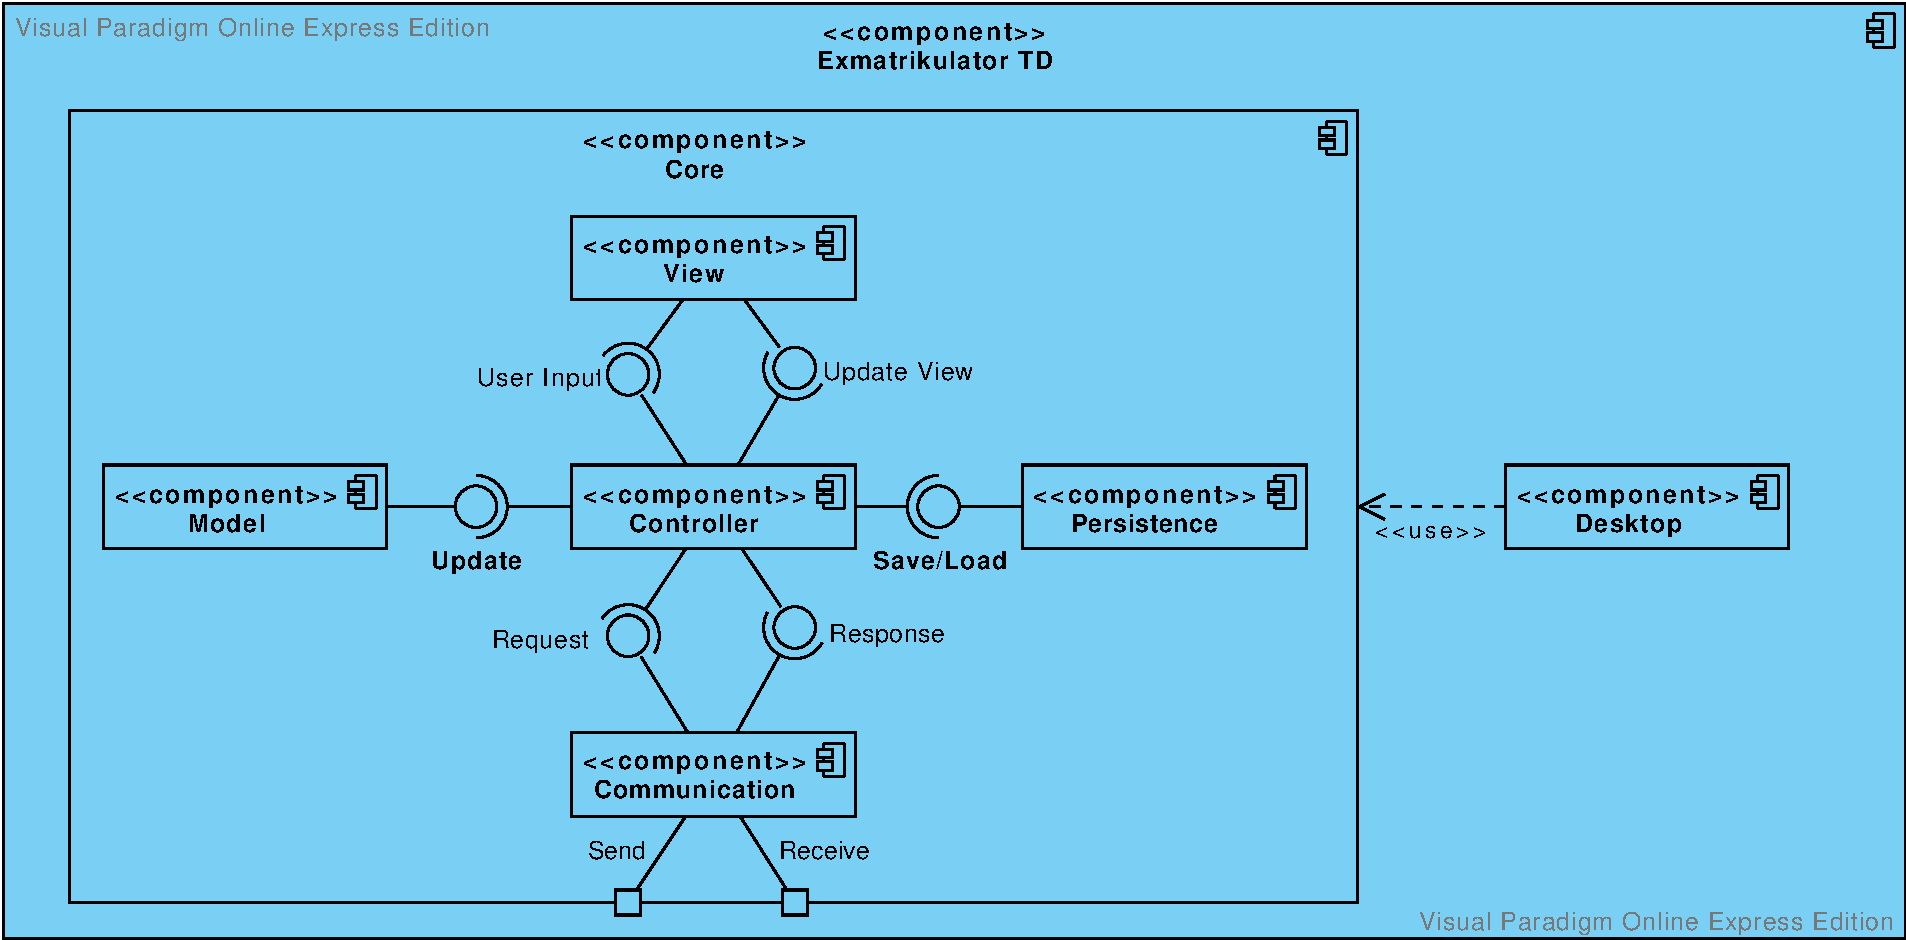
\includegraphics[width=\textwidth]{Bilder/KonzeptionelleSicht.pdf}
    \caption{Konzeptionelle Sicht des Spiels \enquote{Exmatrikulator TD}}
    \label{fig:Komponentendiagramm}
\end{figure}

Wie \autoref{fig:Komponentendiagramm} zu entnehmen ist, ziehen wir zur Realisierung unseres Spiels \enquote{Exmatrikulator TD} wie in Strategie \ref{strat:Core-Komponente} beschrieben zwei Komponenten heran: Eine Komponente \enquote{Core}, die das eigentliche Spiel umsetzt, und eine Komponente \enquote{Desktop}, die das Implementieren von plattformspezifischen Funktionen ermöglicht, im Wesentlichen jedoch der Bereitstellung eines entsprechenden \enquote{Launchers} dient. Diese Struktur der Software ermöglicht es uns, das Spiel später auf zusätzliche Plattformen wie Android oder iOS zu portieren, indem wir entsprechende Komponenten nach dem Vorbild des Desktop-Moduls hinzufügen (siehe hierzu auch \autoref{sec:evolution} zur Evolution der Software). Diese Struktur ergibt sich auch zu einem wesentliche Teil aus der Strategie XYZ \enquote{Nutzung von LibGDX}, da dies die Standard-Struktur eines Projektes ist, das mit diesem Framework erstellt wird.

Die \enquote{Core}-Komponente ist folglich das Herz unserer Software und ist in weitere Komponenten ausdifferenziert, die jeweils eine bestimmte Aufgabe innerhalb des Spieles übernehmen:

\begin{itemize}
    \item Die Komponente \textbf{View} stellt die grafische Benutzeroberfläche zur Verfügung, mit der die Benutzerin interagiert und verwaltet zudem die verschiedenen \enquote{Bildschirme} (Screens), die der Benutzerin angezeigt werden, wie zum Beispiel Menüs oder den eigentlichen Spielbeschirm sowie die grafische Repräsentation der Gegner und Türme. Die View nimmt Eingaben und Spielzüge entgegen und reicht sie an das \textbf{Controller}-Modul weiter, dessen Zustand es zur Darstellung des Spieles rendert. Die Realisierung als eigene Komponente ergibt sich aus den Strategien XYZ \enquote{Kapselung der Benutzerschnittstelle} und ZXY \enquote{Trennung von Datenmodell und grafischer Darstellung}.
    \item Die Komponente \textbf{Controller} dient der Verarbeitung von Benutzereingaben und insbesondere zur Verarbeitung von getätigten Spielzügen und Berechnung des aktuellen Spielzustandes. Es greift auf die Komponente \enquote{Model} zu, das die Spielwelt sowie die verschiedenen Turm- und Einheiten-Typen beinhaltet. In einem Multiplayer-Spiel kann unsere Software sowohl als Client als auch als Server auftreten (Strategie XYZ, \enquote{Kombinierung von Client und Server}). Im ersteren Fall sendet die Game-Logic-Komponente Spielzüge über die Komponente \enquote{Communication} an den Server, der diese verarbeitet, überprüft und (falls es sich um einen legalen Spielzug gehandelt hat) zur Anpassung des Spielzustandes nutzt. Nach Verarbeitung der Anfrage sendet der Server eine passende Antwort, die Informationen über den Erfolg der Anfrage sowie über die konkreten Änderungen am Spielzustand beinhaltet. Die Spielzüge der Spielerin, die die Serverinstanz nutzt, werden wie im Einzelspielermodus direkt an den Controller zur Prüfung weitergegeben. Unter Nutzung der Komponente \enquote{Persistence} wird letztlich der aktuelle Spielzustand auf eine Datenbank abgebildet und kann abgespeichert und wieder geladen werden.
    \item Die Komponente \textbf{Communication} dient der Realisierung der Netzwerkkommunikation stellt sowohl Client- als auch Server-Funktionalität zur Verfügung (vgl. Strategie \ref{strat:kryonet}). Die Realisierung als eigene Komponente dient der Abstraktion der Netzwerkschnittstelle und ermöglicht es uns, diese Komponente weitgehend unabhängig von anderen Teilen des Programmes zu realisieren (Strategie XYZ). Dies erleichtert nicht nur ggf. einen späteren Austausch des verwendeten Frameworks, sondern verringert auch dessen Einfluss auf den Rest der Architektur (Strategie XYZ). Zudem kann durch eine Modularisierung der Software (nicht nur bei dieser Komponente) arbeitsteilig vorgegangen werden (Strategie Blah).
    \item Die Komponente \textbf{Persistence} schließlich dient der Realisierung der Datenhaltung und stellt eine Schnittstelle zu einer eingebetteten Datenbank zur Verfügung. Die Persistence-Komponente abstrahiert dabei vom verwendeten Datenbank-System und erleichtert die Interaktion mit dieser Komponente gemäß Strategie XYZ. 
\end{itemize}

%In \autoref{fig:Komponentendiagramm} ist die konzeptionelle Sicht unserer Software dargestellt. Die gesamte Anwendung läuft auf einem lokalen System, das sich in die Anwendung selbst und die über eine Apache Derby realisierte relationale Datenbank unterteilen lässt. In der Anwendung gibt es drei Komponenten, die das grafische Benutzerinterface, die Befehle zur Bearbeitung des Diagramms sowie einen Persistenz-Komponenten zur Interaktion mit der Datenbank gliedert.

\clearpage

% {\it Diese Sicht beschreibt das System auf einer hohen Abstraktionsebene,
% d.\,h. mit sehr starkem Bezug zur Anwendungsdomäne und den geforderten
% Produktfunktionen und \linebreak-attributen. Sie legt die Grobstruktur fest,
% ohne gleich in die Details von spezifischen Technologien abzugleiten.
% Sie wird in den nachfolgenden Sichten konkretisiert und verfeinert. Die
% konzeptionelle Sicht wird mit {UML}-Komponentendiagrammen visualisiert.}

\section{Modulsicht}

\label{sec:modulsicht}

In diesem Abschnitt gehen wir darauf ein, wie die Komponenten der \enquote{Exmatrikulator TD} zunächst auf Pakete abgebildet werden und wie die geforderten Produkteigenschaften letztlich in einzelnen Modulen umgesetzt werden sollen. Dabei gehen wir Schritt für Schritt vor und erläutern zuerst die Struktur einzelner 

\begin{figure}[H]
    \centering
    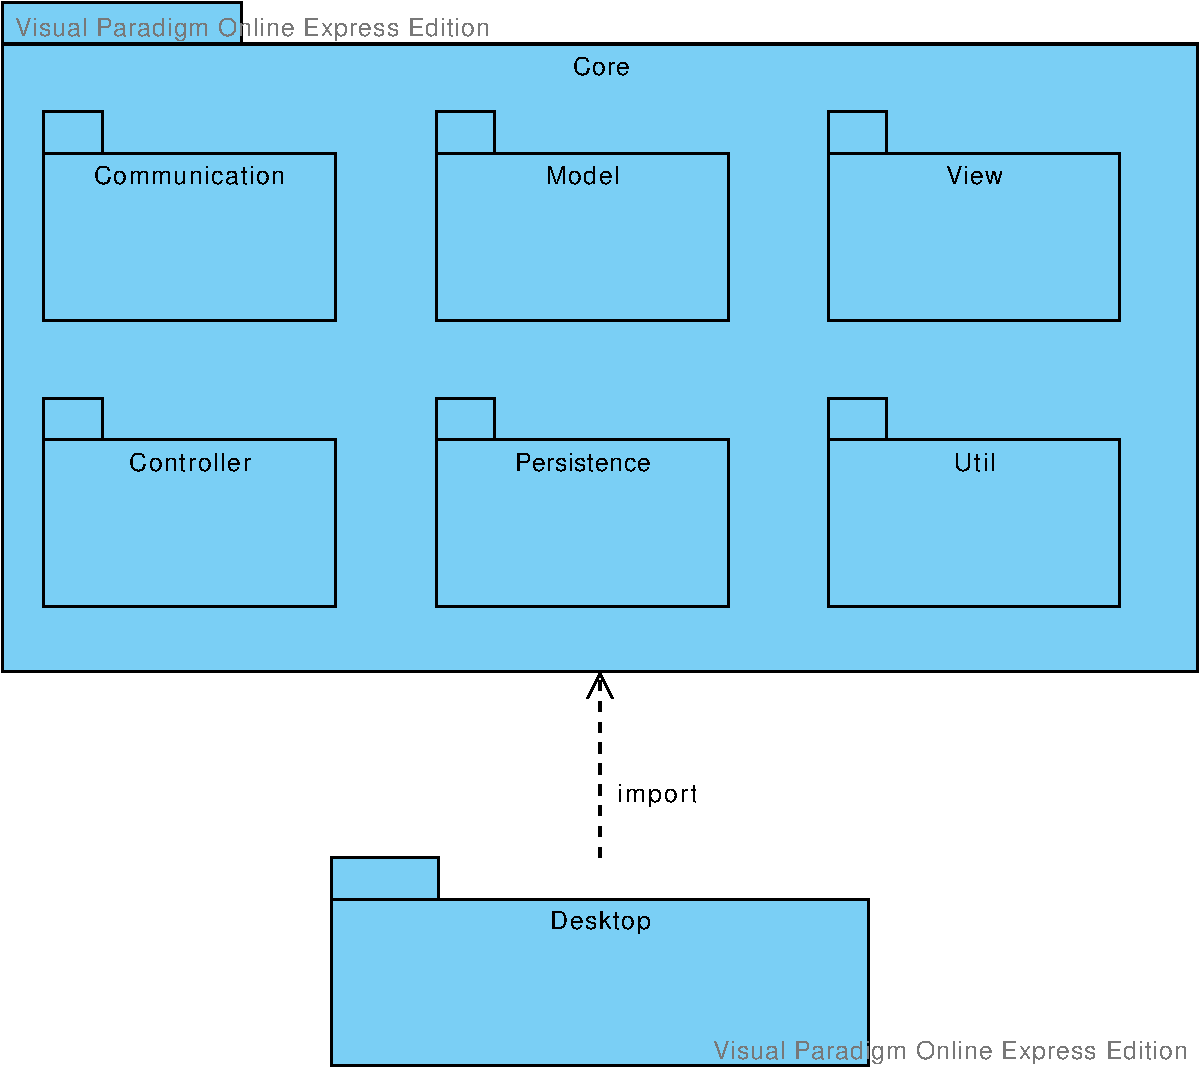
\includegraphics[width=\textwidth]{Bilder/Modulsicht.pdf}
    \caption{Modulsicht des Spiels \enquote{Exmatrikulator TD}}
    \label{fig:Paketdiagramm}
\end{figure}



\subsection{Konkretisierung Desktop}

\label{subsec:desktop}

\begin{figure}[H]
    \centering
    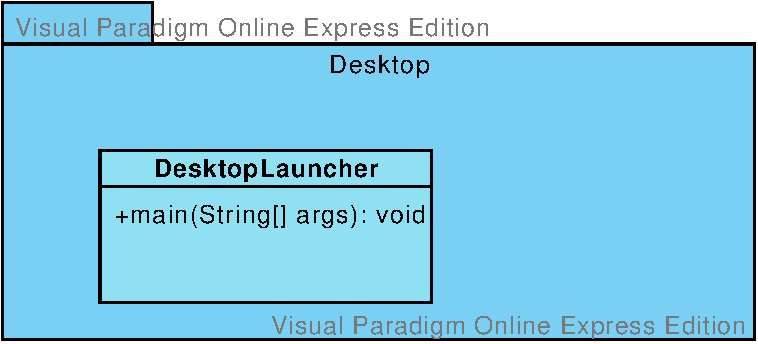
\includegraphics[width=.5\textwidth]{Bilder/Desktop-Modul.pdf}
    \caption{Konkretisierung des Desktop-Moduls}
    \label{fig:desktopModul}
\end{figure}

Das Paket \enquote{Desktop} beinhaltet lediglich ein Modul, den \texttt{DesktopLauncher}. Dieser stellt über eine \textbf{public static void main(String[] args}-Methode den Einstiegspunkt in unsere Software in Desktop- bzw. JVM-Umgebungen dar. Der DesktopLauncher import die Klasse \texttt{ExmatrikulatorTD} aus dem Core-Paket, erzeugt ein \textit{ExmatrikulatorTD}-Objekt und übergibt dieses an ein vom LibGDX-Framework bereitgestelltes \texttt{LwjglApplication}-Objekt, das mit den System-Schnittstellen interagiert. Die eigentliche Funktionalität des Spieles findet sich -- wie bereits erwähnt -- im Core-Paket, das im nachfolgenden Abschnitt ausführlich erläutert wird.

\subsection{Konkretisierung Core}
\label{subsec:core}

\begin{figure}[ht]
    \centering
    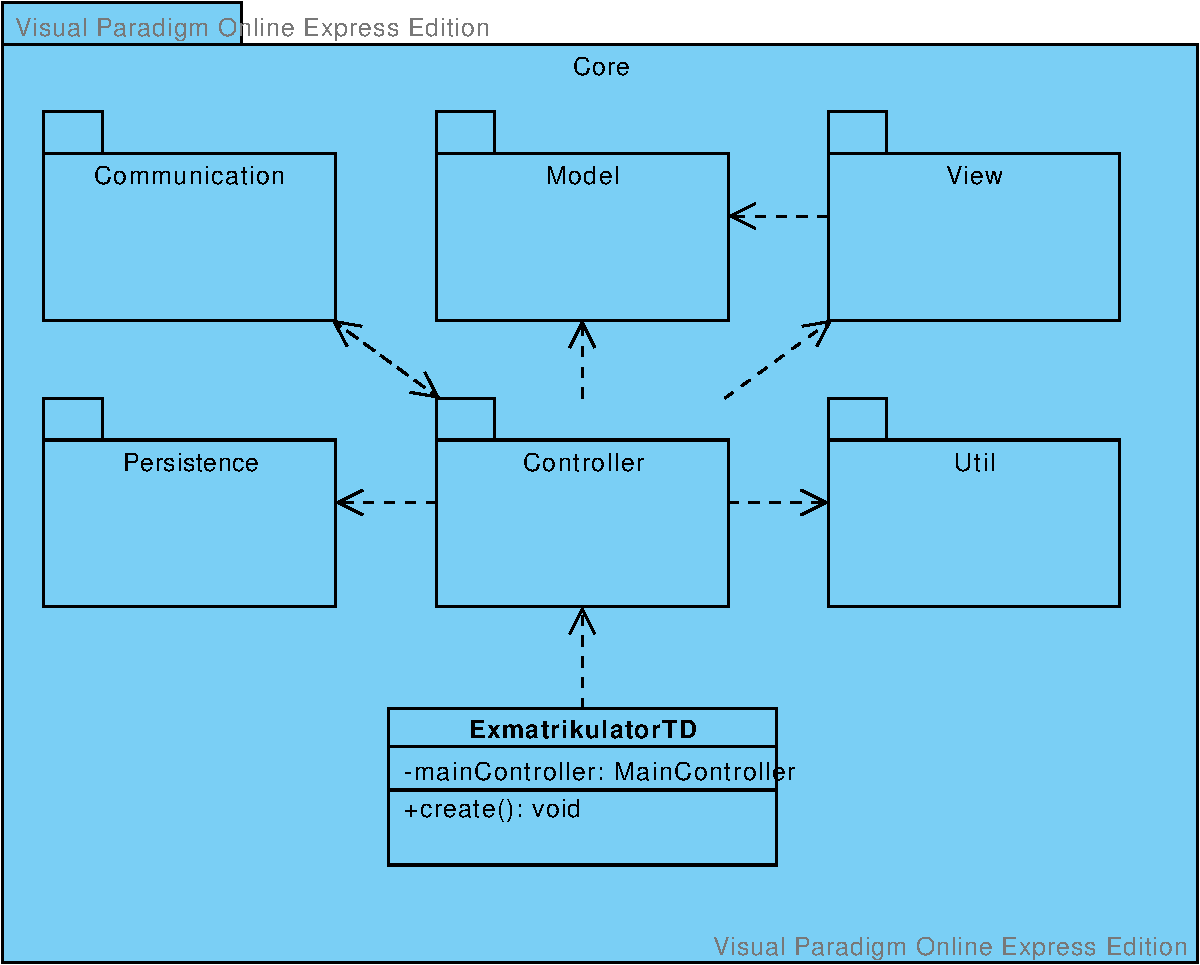
\includegraphics[width=.75\textwidth]{Bilder/CorePaket.pdf}
    \caption{Konkretisierung der Core-Komponente}
    \label{fig:coreModul}
\end{figure}

Das Core-Paket (siehe \autoref{fig:coreModul}) besteht aus den Paketen \textbf{Communication}, \textbf{Model}, \textbf{View}, \textbf{Controller} und \textbf{Persistence}, die eine Abbildung der im letzten Abschnitt vorgestellten Komponenten darstellen. Zusätzlich findet sich im Core-Paket noch ein \textbf{Util}-Paket, das Hilfsklassen beinhaltet sowie die bereits im letzten Abschnitt erwähnte Klasse \texttt{ExmatrikulatorTD}.

\texttt{ExmatrikulatorTD} erbt von der Klasse \texttt{Game} des LibGDX-Frameworks und stellt uns darüber nicht nur eine Schnittstelle für die Darstellung des Spieles und das Anzeigen seiner verschiedenen Bildschirme (\texttt{Screen}s), sondern auch den sogenannten \enquote{Game Loop} zur Verfügung, der in einer Endlosschleife die aktuell vorhandenen grafischen Elemente \texttt{render}t, die in der Regel über die \texttt{Screen}-Objekte selbst verwaltet werden.

In unserer Architektur erzeugt unser \texttt{ExmatrikulatorTD}-Objekt nach dessen Erstellung ein \texttt{MainController}-Objekt und übergibt diesem Verwaltung der Geschäftslogik und der Bildschirme. Dies korrespondiert direkt mit der von uns gewählten Strategie \ref{strat:MVC} und der Nutzung des MVC-Patterns. Wie den in \autoref{fig:coreModul} eingezeichneten Abhängigkeiten zu entnehmen ist, stellt das \texttt{Controller}-Paket den Dreh- und Angelpunkt unserer Architektur dar, weshalb wir uns im nachfolgenden Unterabschnitt der Konkretisierung dieses Paketes widmen werden.

\subsubsection{Konkretisierung des Controller-Pakets}
%Abb noch in arbeit
\begin{figure}[h]
    \centering
    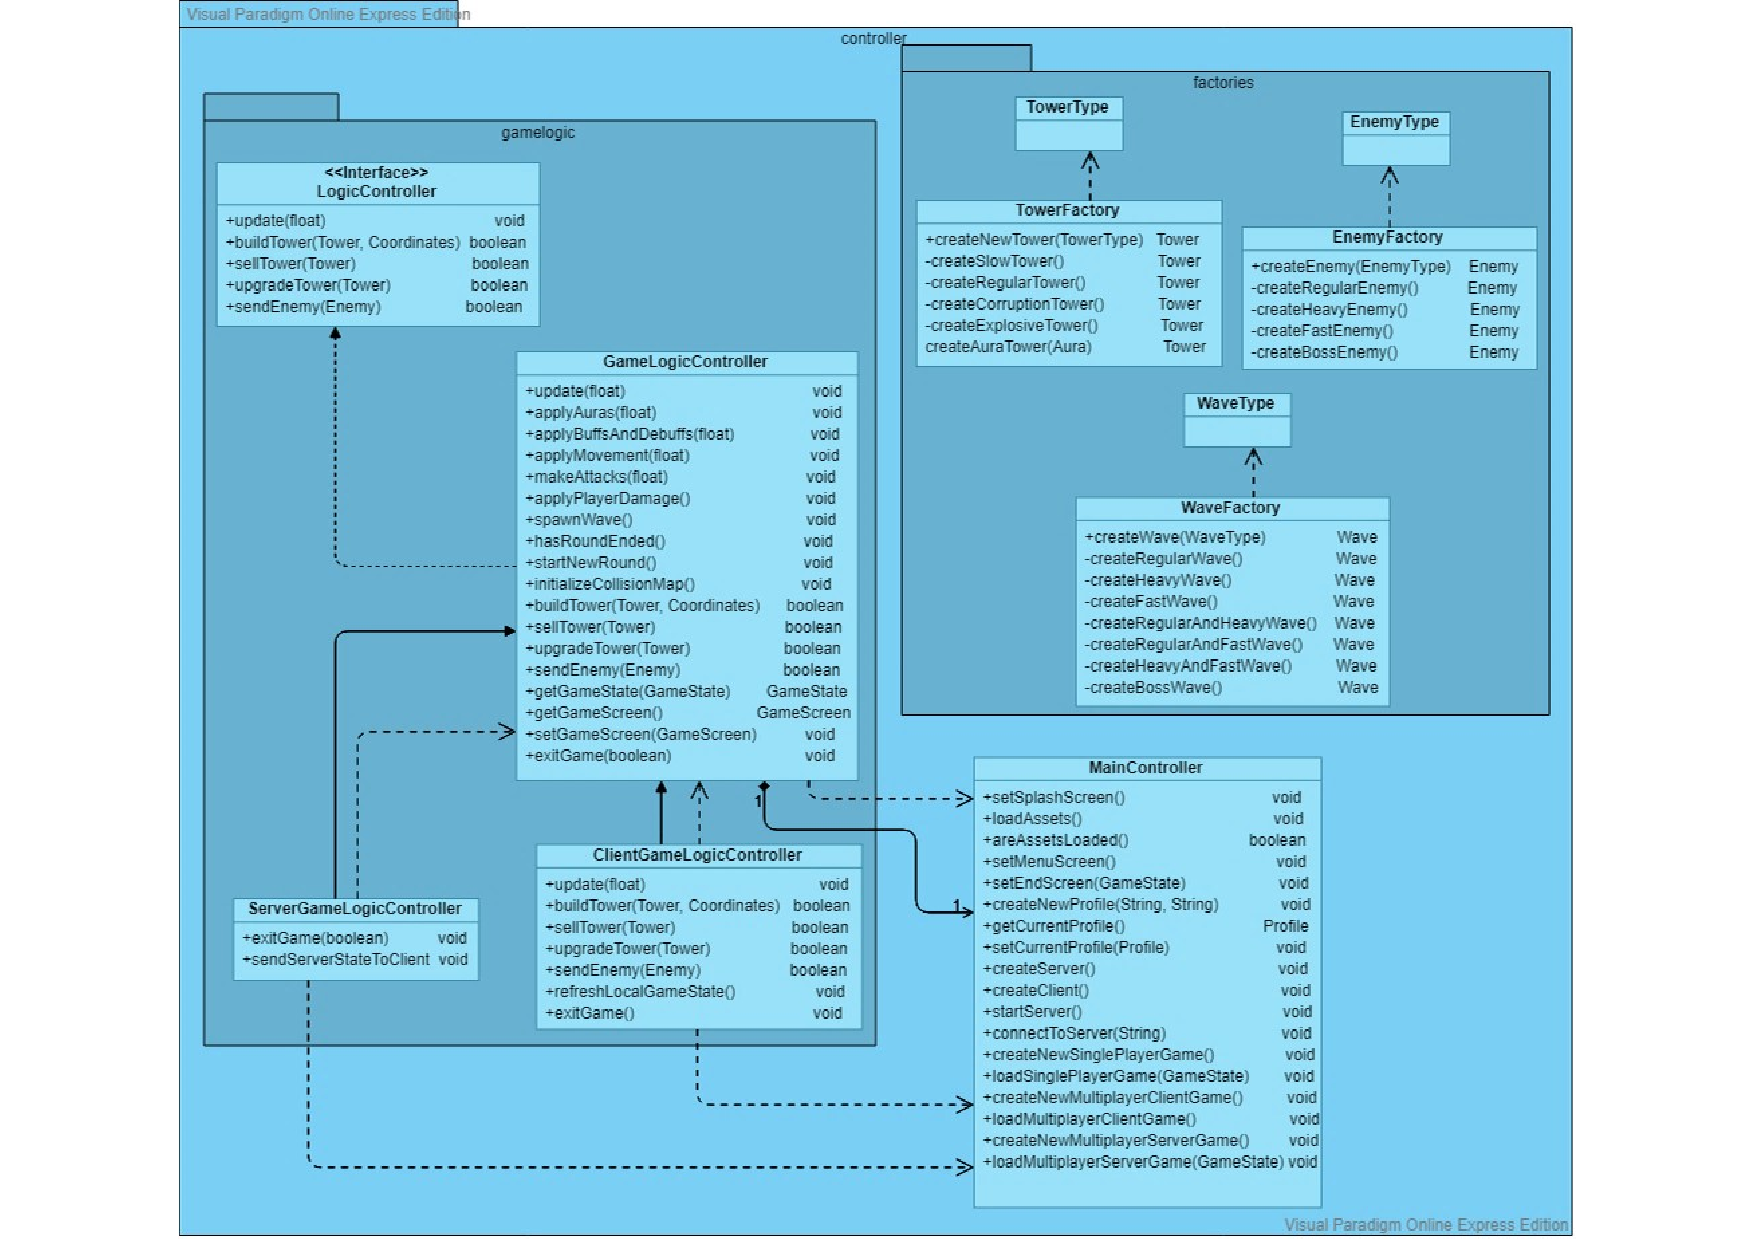
\includegraphics[width=\textwidth]{Bilder/KlassendiagramController.pdf}
    \caption{Konkretisierung des Controller-Pakets}
    \label{fig:contrPak}
\end{figure}

Das Controller-Paket übernimmt die allgemeine Verwaltung der Software über das Modul \texttt{MainController} und realisiert die eigentliche Spiellogik. Neben der \texttt{MainController}-Klasse beinhaltet es ein Unterpaket \texttt{GameLogic}, in dem die Schnittstelle und die Klassen für die Controller der Spiellogik zu finden sind sowie ein Paket \texttt{factories}, in dem \enquote{Factory}-Klassen für die Erstellung von Türmen, Gegnern und Gegnerwellen zu finden sind. 

Das \texttt{MainController}-Modul ist der Dreh- und Angelpunkt für die Verwaltung von Bildschirmen (\texttt{Screens}) und die Verarbeitung von Eingaben über das grafische Benutzerinterface. Es verfügt über Methoden, um Bildschirme zu aktivieren (z.\,B. durch \texttt{public void showMenuScreen()}), die Netzwerkkommunikation zu initialisieren (z.\,B. durch \texttt{public void createClient()} und \texttt{public void connectToServer(String host)}) und neue Spiele zu starten (im Einzelspielermodus mit \texttt{public void createNewSinglePlayerGame ()}) oder Spielstände zu laden (z.\,B. durch \texttt{public void loadSinglePlayerGame (Gamestate gamestate)}). Wird ein Spiel gestartet, gibt der \texttt{MainController} die Kontrolle weitgehend an einen \textit{LogicController} ab, der die Verwaltung des Spielbildschirms und des Spielzustandes übernimmt.

Über einen sogenannten \texttt{AssetManager}, der vom LibGdx-Framework zur Verfügung gestellt wird, verwaltet er zudem die grafischen Ressourcen, aber auch die Audio-Dateien und Schriftarten, die vom Spiel genutzt werden. 

\textbf{Paket Gamelogic}

Dieses Paket beinhaltet Klassen, die den Spielzustand und seine grafische Repräsentation verwalten. Sie stellt zunächst das Interface \texttt{LogicController} bereit, das eine Schnittstelle bietet, über die der \texttt{GameServer} eingegangene Spielzüge an den Controller der Server-Instanz und der \texttt{GameClient} Antworten des Servers an den lokalen Controller weiterleiten kann. Das Interface wird von der Hauptklasse \texttt{GameLogicController} implementiert, die einerseits der Controller für Einzelspieler-Partien und andererseits die Klasse ist, von der die server- beziehungsweise clientspezifischen Controller erben.

Um auf die Server-Verbindung während des Spieles zugreifen zu können, verfügt das Paket über einen expliziten \texttt{ServerGameLogicController}, der vom allgemeinen \texttt{GameLogicController} erbt und dessen Konstruktor zusätzlich eine \texttt{GameServer}-Objekt entgegennimmt. Auf der Client-Seite gibt es analog hierzu einen \texttt{ClientGameLogicController}, dessen Konstruktor ein \texttt{GameClient}-Objekt entgegennimmt, über dessen Schnittstelle die Prüfung von Spielzügen an den Server delegiert wird. Zu diesem Zweck überschreibt der \texttt{ClientGameLogicController} die allgemeinen Methoden für die Ausführung von Spielzügen, die die folgenden Aktionen durchführen:

\begin{itemize}
    \item \texttt{public boolean buildTower (Tower tower, Coordinates coordinates)} baut einen neuen Turm an anzugebenden Koordinaten auf dem Spielfeld.\footnote{Wie auch dem Datenmodell zu entnehmen ist, handelt es sich dabei nicht um pixelbezogene x- und y-Koordinaten, sondern um Felder wie auf einem Schachbrett.} Diese Methode -- wie auch die nachfolgenden drei -- gibt \texttt{true} zurück, wenn der Spielzug legal beziehungsweise erfolgreich war

    \item \texttt{public boolean sellTower (Tower tower)} verkauft einen Turm, indem er (bei Erhöhung des Ressourcenbestandes der jeweiligen Spielerin) aus dem Spiel entfernt wird

    \item \texttt{public boolean upgradeTower (Tower tower)} rüstet einen angegebenen Tower auf die nächste Stufe auf
    
    \item \texttt{public boolean sendEnemy (Enemy enemy)} schickt einen Gegner an die andere Spielerin
\end{itemize}

Gibt der Server nach der Ausführung eine positive Antwort (beziehungsweise \texttt{Response}), erfolgt über den \texttt{GameClient} und die \texttt{LogicController}-Schnittstelle auch lokal die Durchführung des Spielzuges, die zur Aktualisierung des Spielzustandes führt.\footnote{Hierfür ist es allerdings erforderlich, dass die entsprechenden Request- beziehungsweise Response-Listener in \texttt{GameClient} und \texttt{GameServer} mit dem jeweiligen LogicController initialisiert wurden.}

Im Singleplayer-Modus übernimmt der allgemeine \texttt{GameLogicController} die Verwaltung des Spielzustandes und führt sämtliche Spielzüge lokal aus. Neben der Ausführung von Spielzügen berechnet der \texttt{GameLogicController} fortwährend im Rahmen des \enquote{Game Loops} (konkret innerhalb der Methode \texttt{public void update(float deltaTime)}) den aktuellen Spielzustand und bewegt beispielsweise über die Methode \texttt{void applyMovement (float deltaTime)} die Einheiten über den Bildschirm oder führt über \texttt{void makeAttacks (float deltaTime)} Angriffe aus. Da der Controller sowohl das \texttt{Model} als auch die \texttt{View} kennt, kann er folglich sowohl den Datenbestand aktualisieren als auch die grafische Darstellung manipulieren. Diese Trennung gemäß MVC-Pattern (Strategie \ref{strat:MVC}) bietet den großen Vorteil, dass die Spiellogik vollkommen unabhängig von der letztlichen grafischen Umsetzung erfolgt, was zum einen ein wesentlich einfacheres Testen und zum anderen ein arbeitsteiliges Vorgehen ermöglicht. Die Abbildung von Türmen und Gegnern des Spielzustandes auf ihre grafische Repräsentation erfolgt dabei im Controller durch die Nutzung von \texttt{HashMap}s, durch die ein sehr effizienter ($\mathcal{O}(1)$) Zugriff von einem Element im Spielzustand auf das jeweils korrespondierende \texttt{GameObject} möglich wird.

\textbf{Paket Factories}

Dieses Paket enthält Module, mit denen sich die verschiedenen Turm, Gegner- und Wellen-Arten erzeugen lassen. Dabei kommt das sogenante Factory-Pattern zum Einsatz (siehe Strategie XYZ), das die Erstellung der jeweiligen Objekte auf entsprechende Methoden abstrahiert, innerhalb derer die Erzeugung definiert wird. Nach außen hin bieten die Factories jeweils eine allgemeine \enquote{createNewObject}-Methode, die ein Objekt einer jeweils definierten  Aufzählungsklasse erwartet, die die verschiedenen Typen von Einheiten, Türmen und Wellen nach außen kommuniziert. Die \texttt{TowerFactory} bietet beispielsweise (aktuell) die Typen \texttt{SLOW\_TOWER, REGULAR\_TOWER, CORRUPTION\_TOWER, EXPLOSIVE\_TOWER} und  \texttt{AURA\_TOWER}. Je nach übergegebenem Objekt kann in der Methode \texttt{public void createNewTower (TowerType towerType)} die passende Erstellungsmethode aufgerufen werden, im Falle es \texttt{SLOW\_TOWER} etwa die Methode \texttt{private Tower createSlowTower ()}. 

\clearpage

\subsubsection{Konkretisierung des View-Pakets}
\begin{figure}[ht]
    \centering
    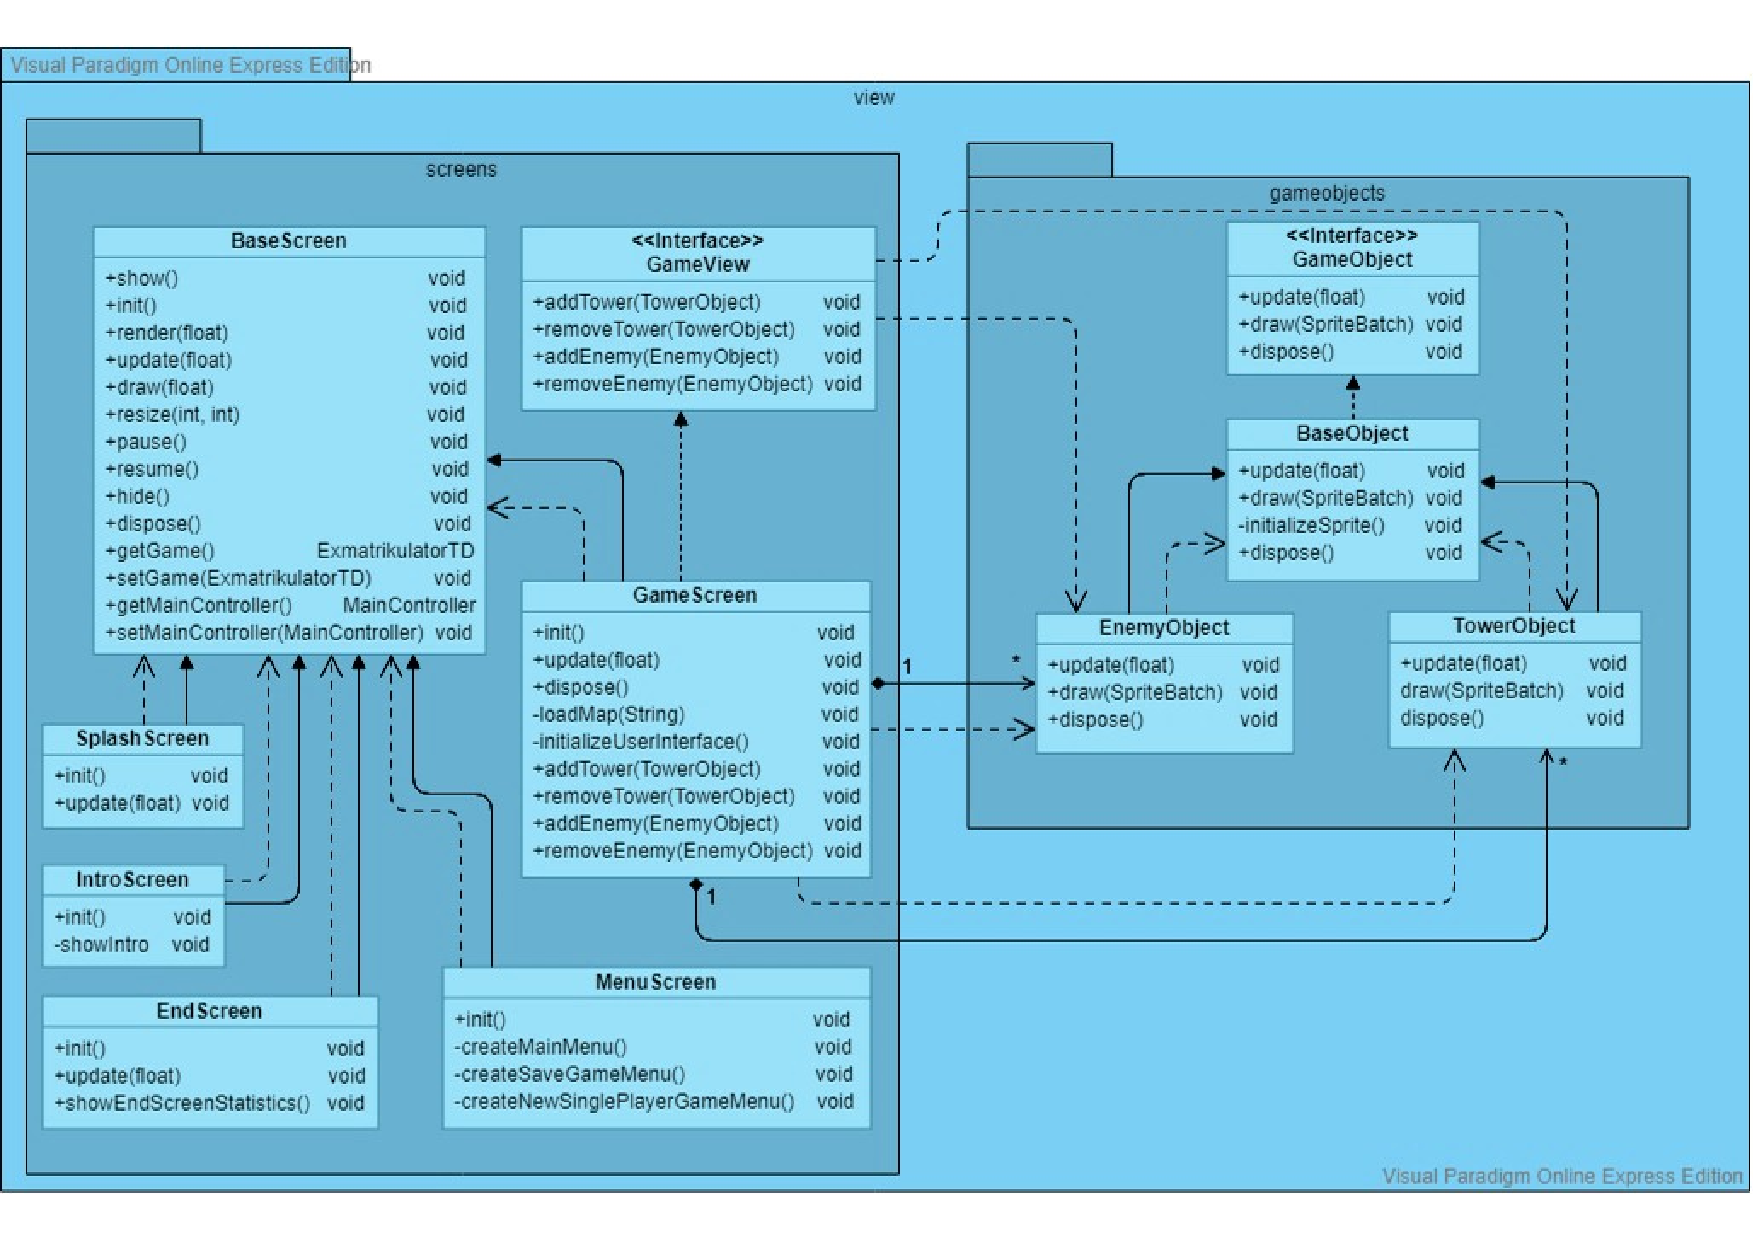
\includegraphics[width=\textwidth]{Bilder/KlassendiagramView.pdf}
    \caption{Konkretisierung des View-Pakets}
    \label{fig:viewPak}
\end{figure}
Das \texttt{View}-Paket ist untergliedert in die Teilpakete beziehungsweise Module \texttt{Screens} und \texttt{Gameobjects}. Im \texttt{Screens}-Paket werden alle interaktiven Menuelemente gemanagt und im \texttt{Gameobjects}-Paket werden die einzelnen interaktiven Spielobjekte (Türme und Gegner) verwaltet.



%Abb so weit fertig, upload erfolgt später
\subsubsection{Konkretisierung des Model-Pakets}

\begin{figure}[H]
    \centering
    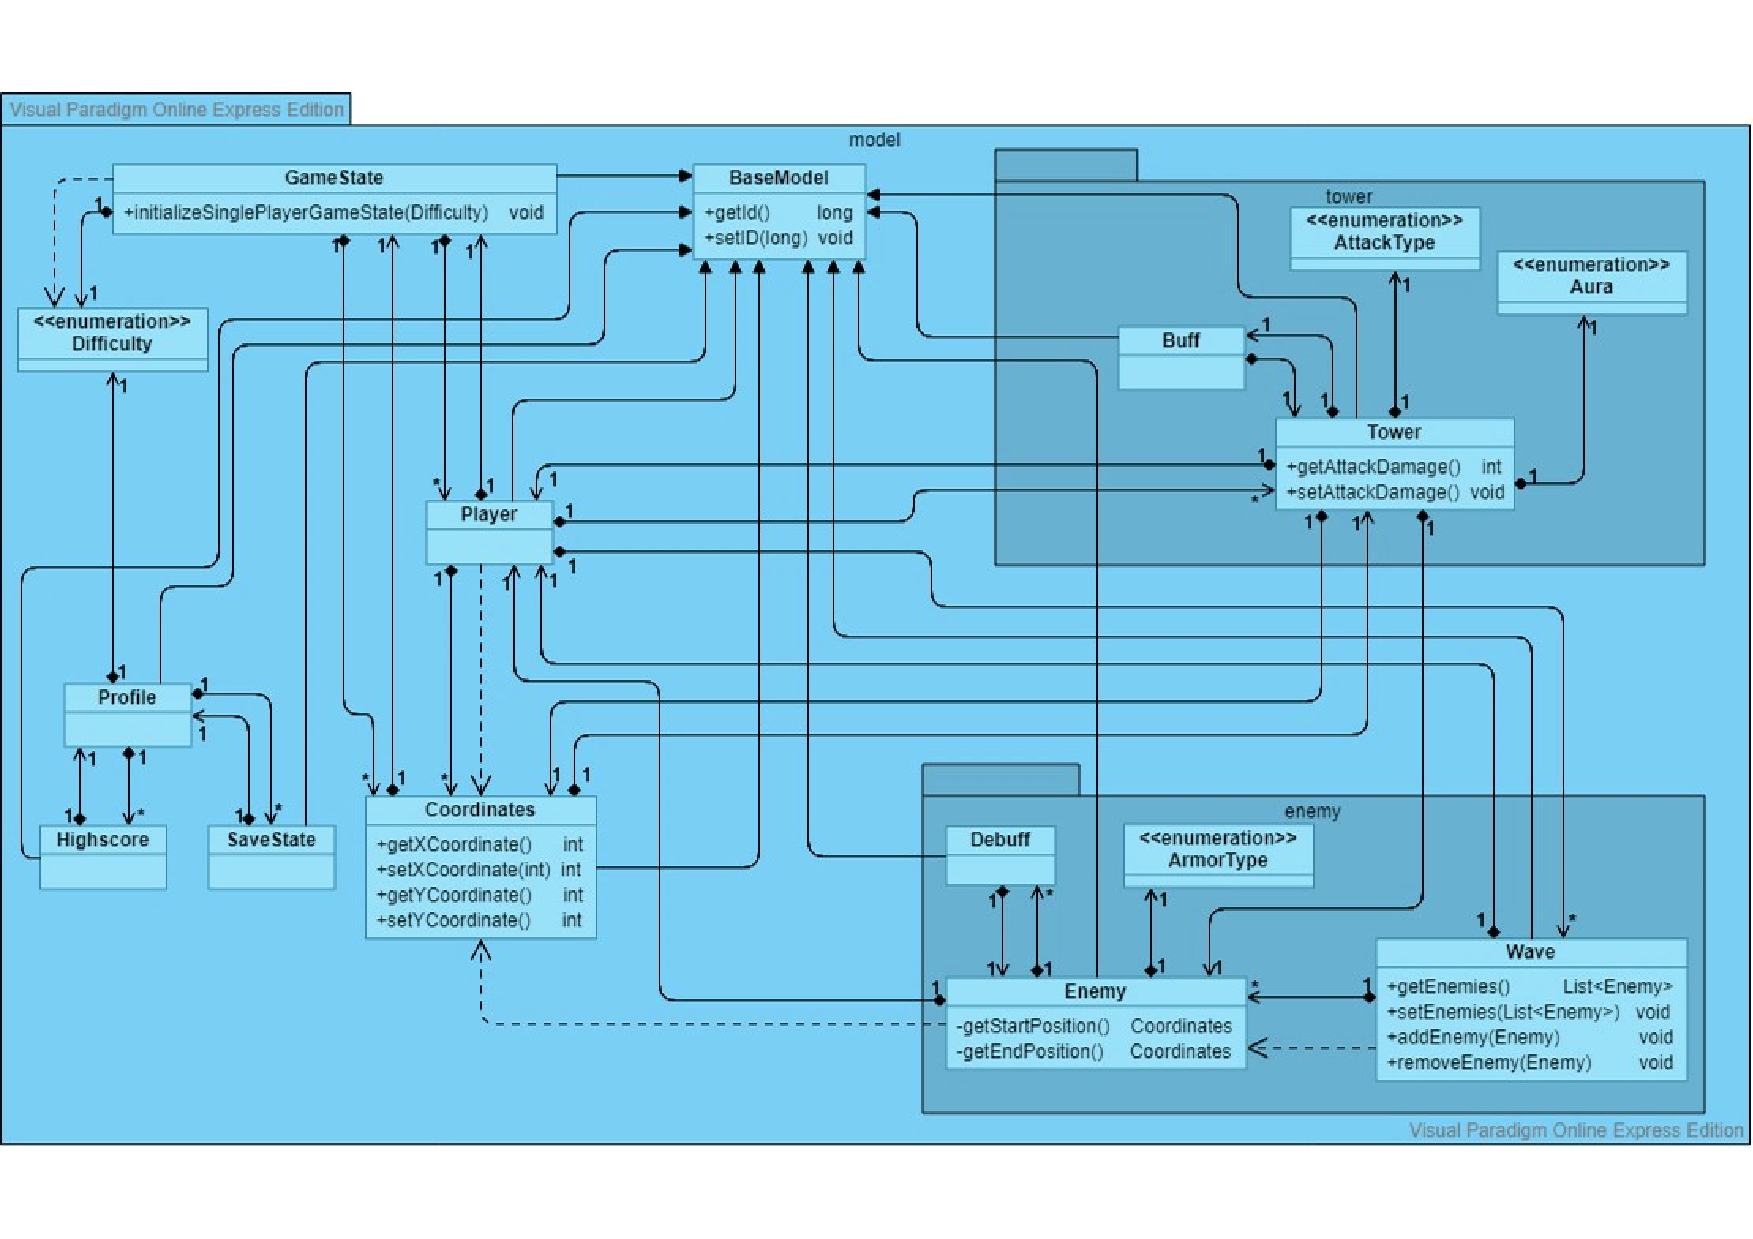
\includegraphics[width=\textwidth]{Bilder/KlassendiagramModel.pdf}
    \caption{Konkretisierung des Model-Pakets}
    \label{fig:modPak}
\end{figure}

Das \texttt{Model}-Paket beinhaltet die grundlegende Datenstruktur für die einzelnen Spielobjekte.
Das Paket ist in zwei weitere untergeordnete Pakete aufgeteilt, \texttt{Enemy} und \texttt{Tower}, welche die spezifischen Strukturen für die Türme und die Gegner beinhaltet.

\subsubsection{Konkretisierung des Communication-Pakets}
\begin{figure}[H]
    \centering
    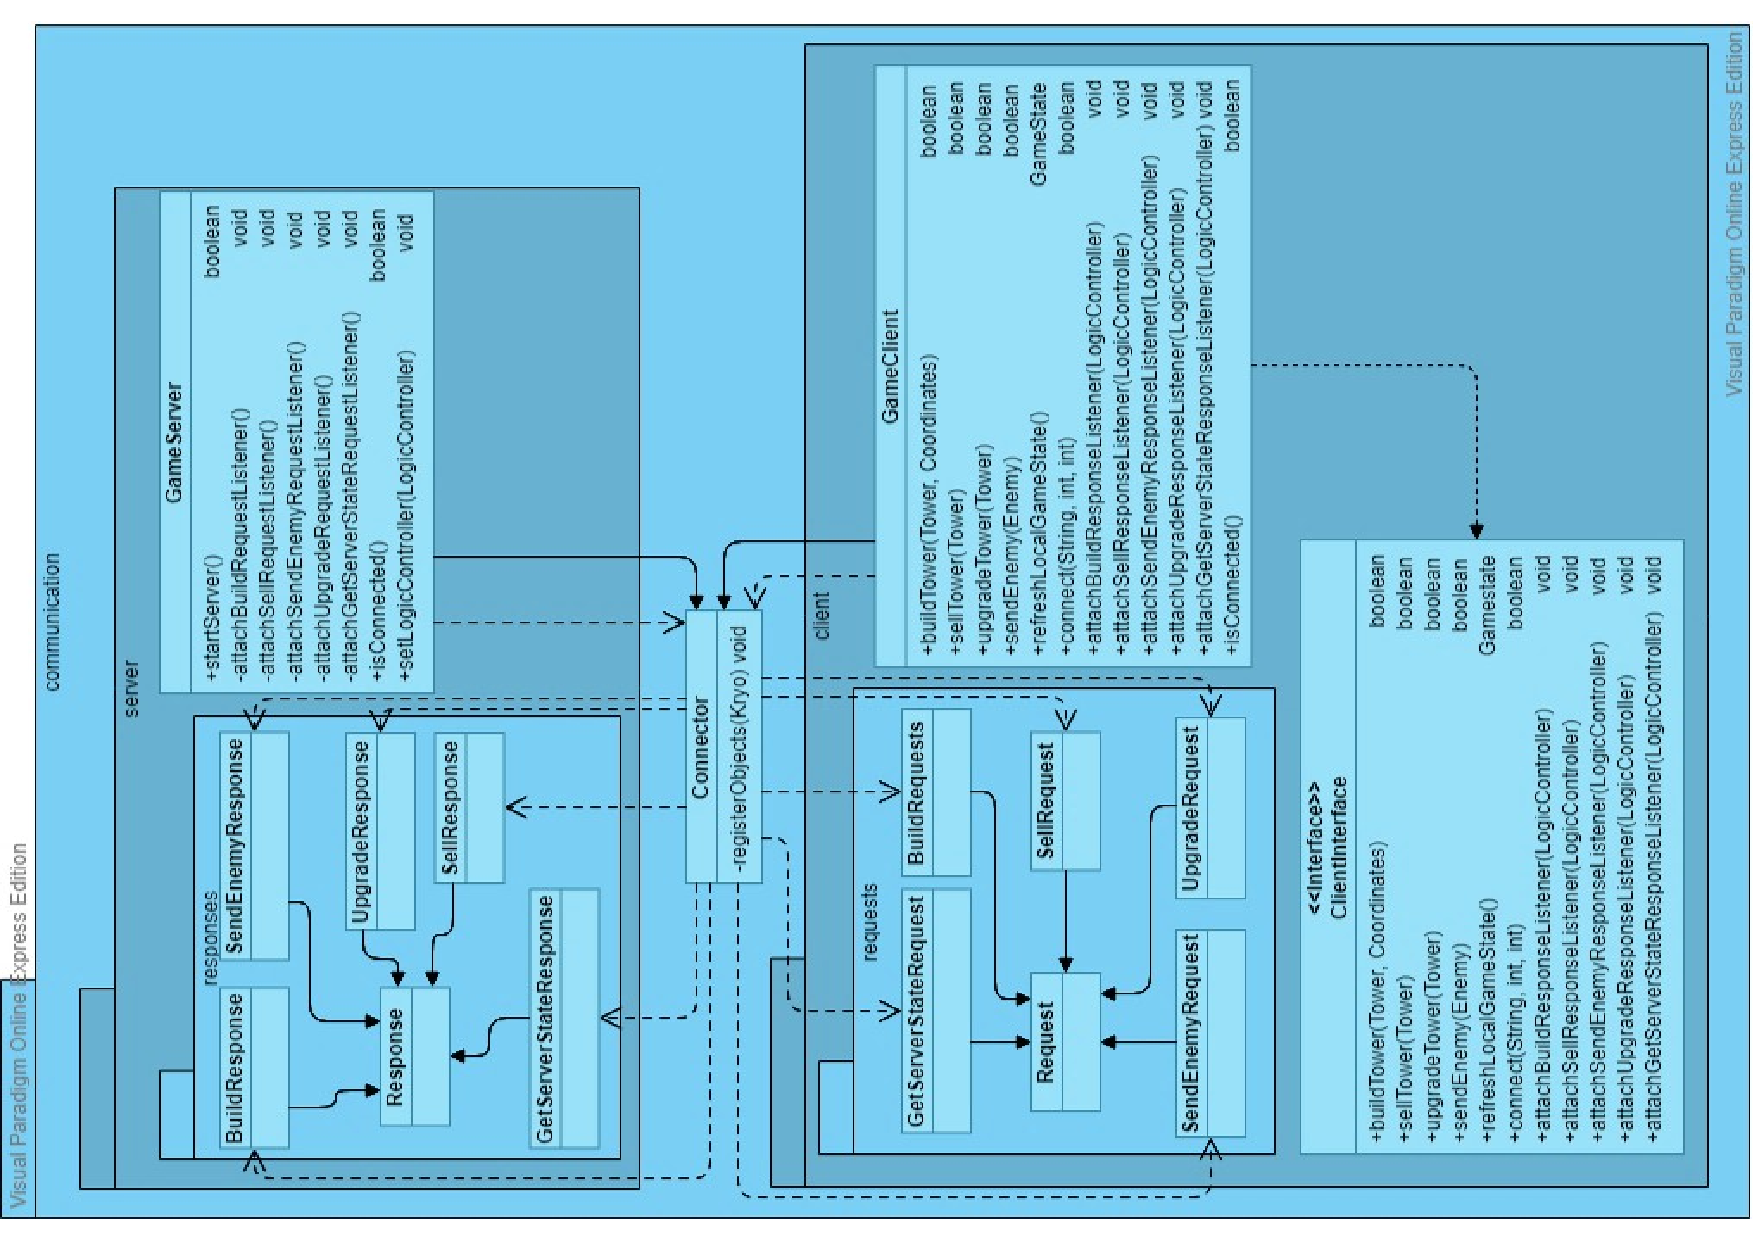
\includegraphics[width=\textwidth, angle=270]{Bilder/KlassenDiagrammCommunication.pdf}
    \caption{Konkretisierung des Communication-Pakets}
    \label{fig:comPak}
\end{figure}
Das \texttt{Communication}-Paket verwaltet die Client-Server Kommunikation. Das Paket beinhaltet zwei weitere Pakete, \texttt{server} und \texttt{client}, über die Client und Server spezifische Aktionen erfolgen.
\subsubsection{Konkretisierung des Persistence-Pakets}
\begin{figure}[H]
    \centering
    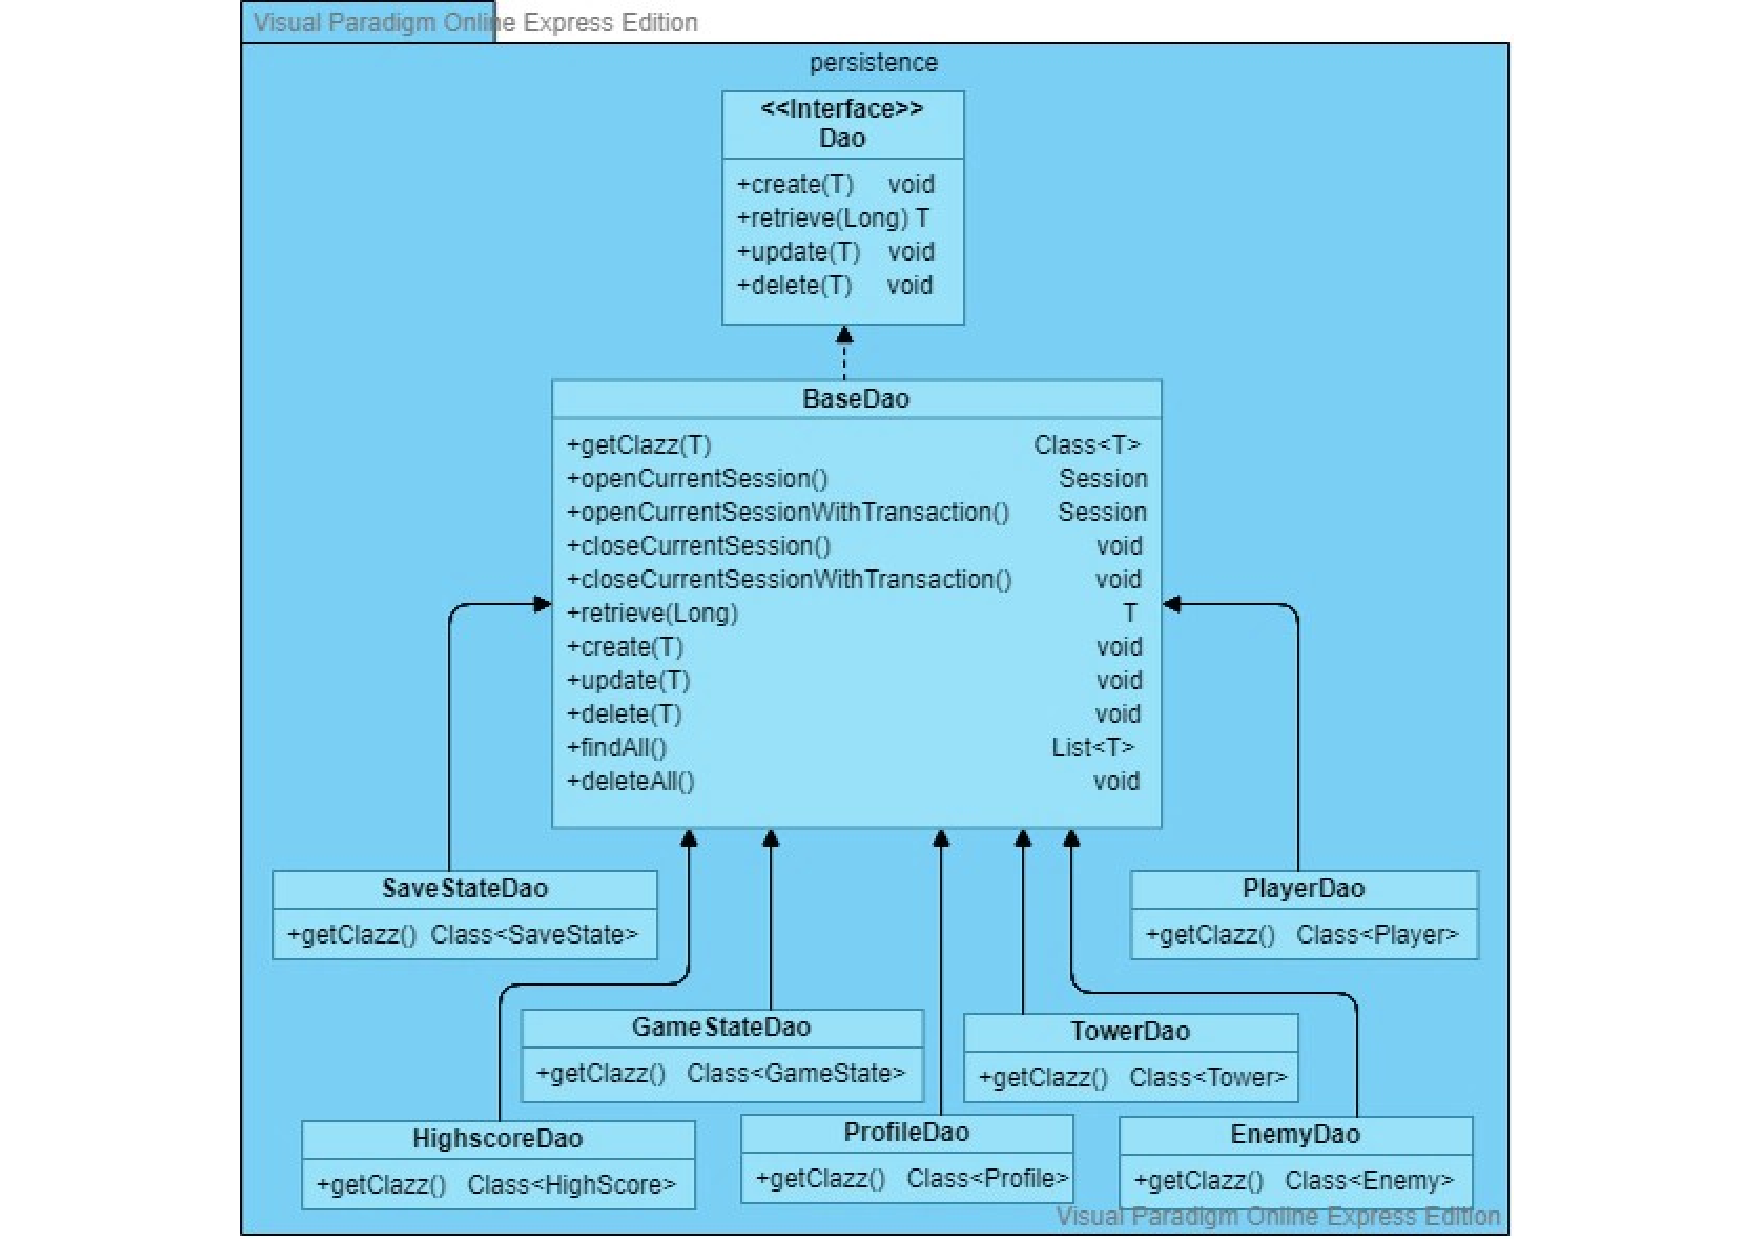
\includegraphics[width=\textwidth]{Bilder/KlassendiagrammPersistence.pdf}
    \caption{Konkretisierung des Persistence-Pakets}
    \label{fig:persPak}
\end{figure}
Das \texttt{Persistence}-Paket stellt über das DAO-Pattern eine Schnittstelle zur Interaktion mit der Datenbank zur Verfügung. Über ein Dao-Interface werden dabei die sogenannte CRUD-Operationen (Create, Retrieve, Update, Delete) bereitgestellt, die das Persistieren, Löschen, Aktualisieren und Abrufen von Java-Objekten beziehungsweise den mit ihnen korrespondierenden Datenbank-Einträgen ermöglichen. Zu jeder relevanten Klasse des \texttt{Model}-Paketes gibt es dabei eine entsprechende Dao-Klasse, die diese Operationen für die jeweiligen Objekttypen ermöglicht.

%Abb so weit fertig, upload erfolgt später
\subsubsection{Konkretisierung des Util-Pakets}
\begin{figure}[H]
    \centering
    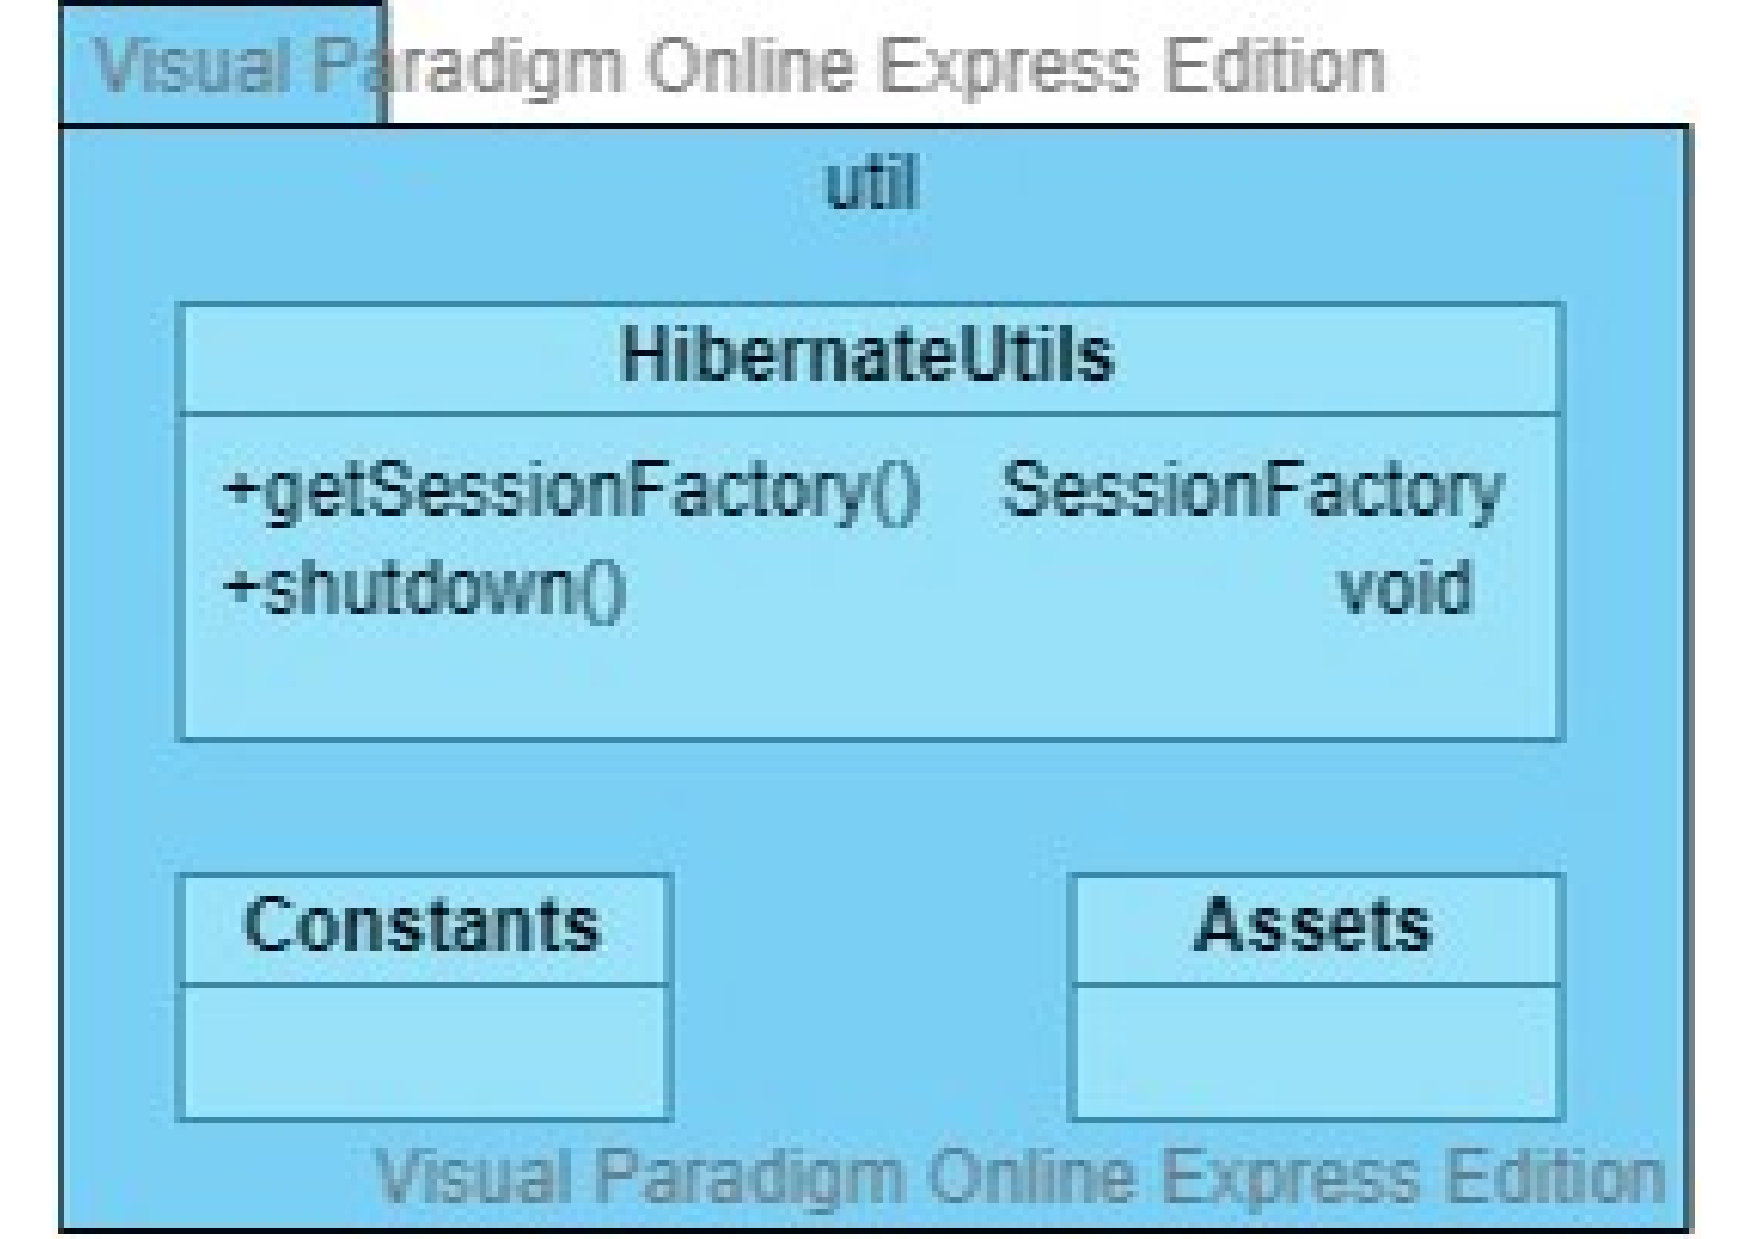
\includegraphics[width=0.5\textwidth]{Bilder/KlassendiagrammUtils.pdf}
    \caption{Konkretisierung des Utils-Pakets}
    \label{fig:utilPak}
\end{figure}

Das Util-Paket stellt vor allem Module mit Konstanten für die Anwendungslogik sowie Bezeichnungen für Assets zur Verfügung. Die Klasse \texttt{HibernateUtils} stellt eine Session-Factory zur Verfügung, über die die Transaktionen mit der Datenbank realisiert werden.

%Abb so weit fertig, upload erfolgt später

%Einfach gesagt lässt sich die Anwendung in 4 Aufgabenbereiche und in unserem Fall in Pakete aufteilen. 
%Die \textbf{graphische Benutzeroberfläche} ({\it graphical user interface} oder GUI) ermöglicht es dem Nutzer entweder Einstellungen zum Programm selbst zu verändern oder mit dem \textbf{Graphen} zu interagieren. Letzteres erfolgt über die Ausführung von \textbf{Befehlen} ({\it Commands}). Ein Command verursacht eine Veränderung am Graphen, welcher dann widerum neu über die GUI dargestellt wird. Der Kunde ist vor allem daran interessiert die Interaktion mit dem Graphen zu protokollieren, d.h. zu verfolgen, welche Befehle wie ausgeführt werden. Dies ist die Aufabe der \textbf{Persistance}, welche die Commands im gewünschten Format in eine beliebige Datenbank speichert. Das Persistance-Framework ermöglicht es Klassen wie Entitäten im Sinne einer Datenbank zu behandeln und erlaubt es uns unabhängig vom Datenbankmanagementsystem Anfragen zu schreiben.

%\subsection{Pakete}
%Seit die Anforderungen aktualisiert wurden und Klarheit darüber bestand, dass lediglich die Interaktion mit dem Graphen in einer Datenbank protokolliert werden soll, wurde die Datensicht des Projekts erheblich eingeschränkt. Deswegen haben wir uns dazu entschieden, die Modulsicht und Datensicht zu vereinen um Redundanz zu vermeiden. Desweiteren wird die Persistance im Folgenden nicht weiter aufgeführt, da diese ziemlich implementierungsspezifisch ist und sich eine entsprechende Wahl erst während der Implementierung ermöglicht.

%\label{sec:pakete}

%\subsubsection{GUI}
% Die GUI setzt sich aus zwei Komponenten zusammen, nämlich dem Hauptfenster und einem Einstellungsdialog. Beide Teile werden mittels Model-View-Controller-Pattern realisiert. Getrennt werden die beiden, weil sie jeweils eine große Anzahl an Komponenten enthalten, ohne dass sie etwas mit dem jeweiligen anderen Bestandteil zu tun haben, und um Modularität zu gewährleisten.\\
% \begin{figure}[H]
%     \centering
%     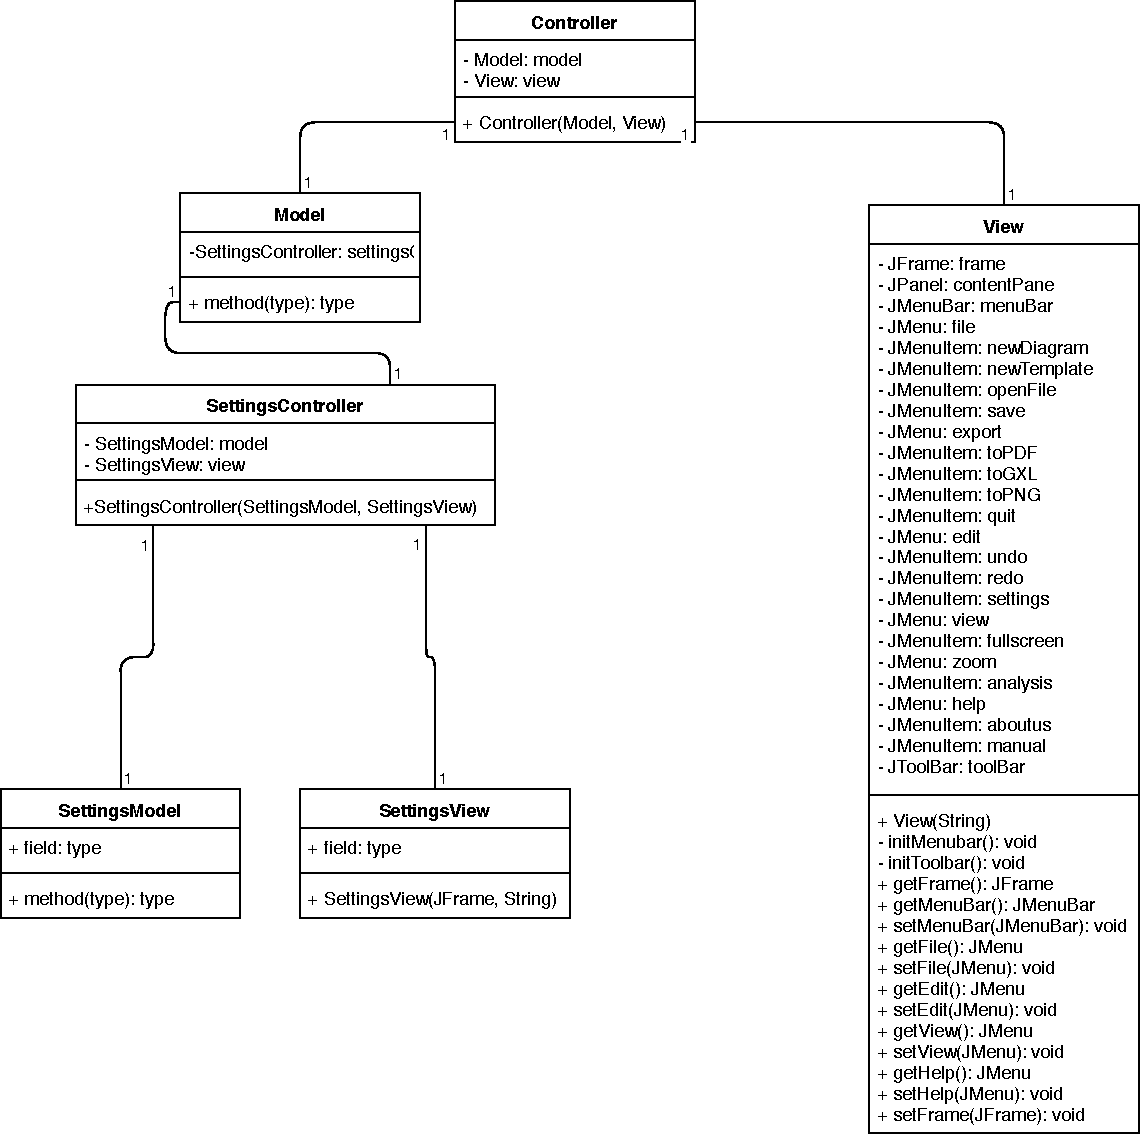
\includegraphics[width=\textwidth]{Bilder/gui_paket.pdf}
%     \caption{GUI-Paket}
%     \label{fig:GUI-Paket}
% \end{figure}

% \newpage

% \subsubsection{Command}
% Um die Protokollierung des Nutzerverhaltens sowie die Undo-Redo-Funktionalität zu ermöglichen, wird das Command-Pattern verwendet. Dabei dient der {\it CommandStack} als Stack für ausgeführte Befehle. Die abstrakte Klasse {\it Command} stellt eine Blaupause für alle Command-Klassen dar. Für jede verändernde Aktion am Graphen gibt es genau einen Command. Jeder dieser Commands hat eine Methode {\it execute}, welche die tatsächliche Aktion realisiert, eine Methode {\it undo}, welche das exakte Gegenteil von {\it execute} ist, um ein Undo zu ermöglichen und eine {\it toString}-Methode für die Ausgabe in einem menschlich-verständlichen Format. Je nachdem welche Funktionalität nachträglich hinzugefügt werden soll, muss lediglich eine von {\it Command} erbende Klasse geschaffen und ein entsprechender Verweis auf diese erzeugt werden.\\
% \begin{figure}[H]
%     \centering
%     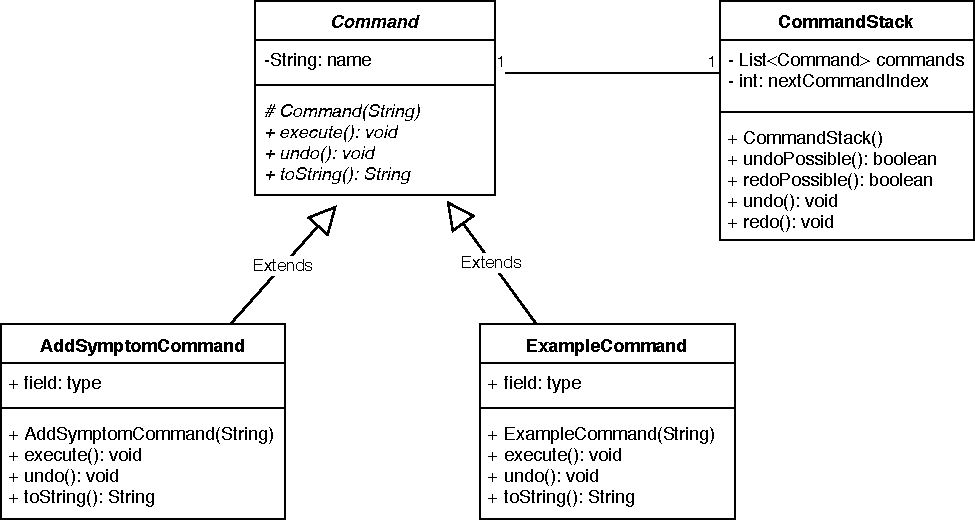
\includegraphics[width=\textwidth]{Bilder/command_paket.pdf}
%     \caption{Command-Paket}
%     \label{fig:Command-Paket}
% \end{figure}

% \newpage

% \subsubsection{Graph}
% Ein Graph (in unserem Falle ein Syndrom) setzt sich zusammen aus einer Liste an {\it Symptom}s. Jedes dieser Symptome gehört zu exakt einer {\it Sphere}. Sowohl Spähren als auch Symptome werden durch Strings betitelt. Jeweils 2 Symptome werden verbunden durch eine Relation, welche einem von 3 verschiedenen Typen entsprechen kann. Alle Klassen enthalten Getter-Setter-Funktionalität für sämtliche Attribute sowie Ausgabe-Funktionalität für eine gewünschte Form der Serialisierung. über {\it Syndrom} lassen sich außerdem die gewünschten Kennzahlen mittels Graph-Algorithmen errechnen.\\
% \begin{figure}[H]
%     \centering
%     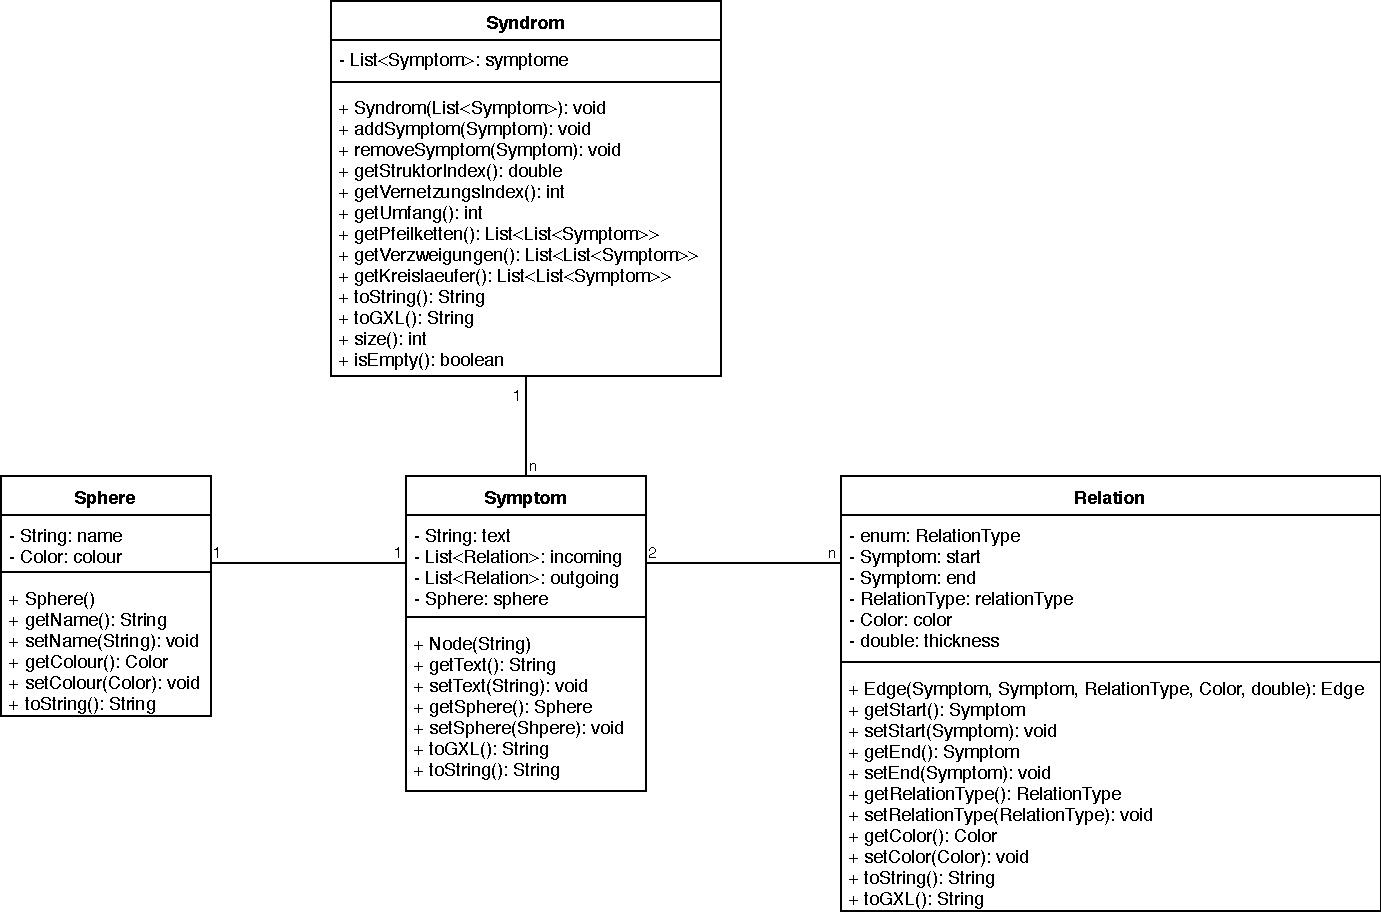
\includegraphics[width=\textwidth]{Bilder/graph_paket.pdf}
%     \caption{Graph-Paket}
%     \label{fig:Graph-Paket}
% \end{figure}

% \newpage

% {\it
% Diese Sicht beschreibt den statischen Aufbau des Systems mit Hilfe von
% Modulen, Subsystemen, Schichten und Schnittstellen.
% Diese Sicht ist hierarchisch, d.\,h. Module werden in Teilmodule
% zerlegt. Die Zerlegung endet bei Modulen, die ein klar umrissenes
% Arbeitspaket für eine Person darstellen und in einer Kalenderwoche
% implementiert werden können. Die Modulbeschreibung der Blätter dieser
% Hierarchie muss genau genug und ausreichend sein, um das Modul
% implementieren zu können.

% Die Modulsicht wird durch {UML}-Paket- und Klassendiagramme visualisiert.

% Die Module werden durch ihre Schnittstellen beschrieben.
% Die Schnittstelle eines Moduls $M$ ist die Menge aller Annahmen, die
% andere Module über $M$ machen dürfen, bzw.\ jene Annahmen, die $M$
% über seine verwendeten Module macht (bzw. seine Umgebung, wozu auch
% Speicher, Laufzeit etc.\ gehören).
% Konkrete Implementierungen dieser Schnittstellen sind das Geheimnis des Moduls
% und können vom Programmierer festgelegt werden. Sie sollen hier
% dementsprechend nicht beschrieben werden.

% Die Diagramme der Modulsicht sollten die zur Schnittstelle gehörenden Methoden
% enthalten. Die Beschreibung der einzelnen Methoden (im Sinne der Schnittstellenbeschreibung)
% geschieht allerdings per Javadoc im zugehörigen Quelltext. Das bedeutet, dass Ihr
% für alle Eure Module Klassen, Interfaces und Pakete erstellt und sie mit den Methoden der
% Schnittstellen verseht. Natürlich noch ohne Methodenrümpfe bzw.\ mit minimalen Rümpfen.
% Dieses Vorgehen vereinfacht den Schnittstellenentwurf und stellt Konsistenz sicher.

% Jeder Schnittstelle liegt ein
% Protokoll zugrunde. Das Protokoll beschreibt die Vor- und
% Nachbedingungen der Schnittstellenelemente. Dazu gehören die erlaubten
% Reihenfolgen, in denen Methoden der Schnittstelle aufgerufen werden
% dürfen, sowie Annahmen über Eingabeparameter und Zusicherungen über
% Ausgabeparameter. Das Protokoll von Modulen wird in der Modulsicht beschrieben.
% Dort, wo es sinnvoll ist, sollte es mit Hilfe von Zustands- oder
% Sequenzdiagrammen spezifiziert werden. Diese sind dann einzusetzen, wenn der
% Text allein kein ausreichendes Verständnis vermittelt (insbesondere
% bei komplexen oder nicht offensichtlichen Zusammenhängen).

% Der Bezug zur konzeptionellen Sicht muss klar ersichtlich sein. Im
% Zweifel sollte er explizit erklärt werden. Auch für diese Sicht muss
% die Entstehung anhand der Strategien erläutert werden.
% }

\clearpage

\section{Datensicht}
\label{sec:datensicht}



\subsection{Konkretisiertes Datenmodell}
\label{subsec:datenmodell}


\begin{figure}[H]
    \centering
    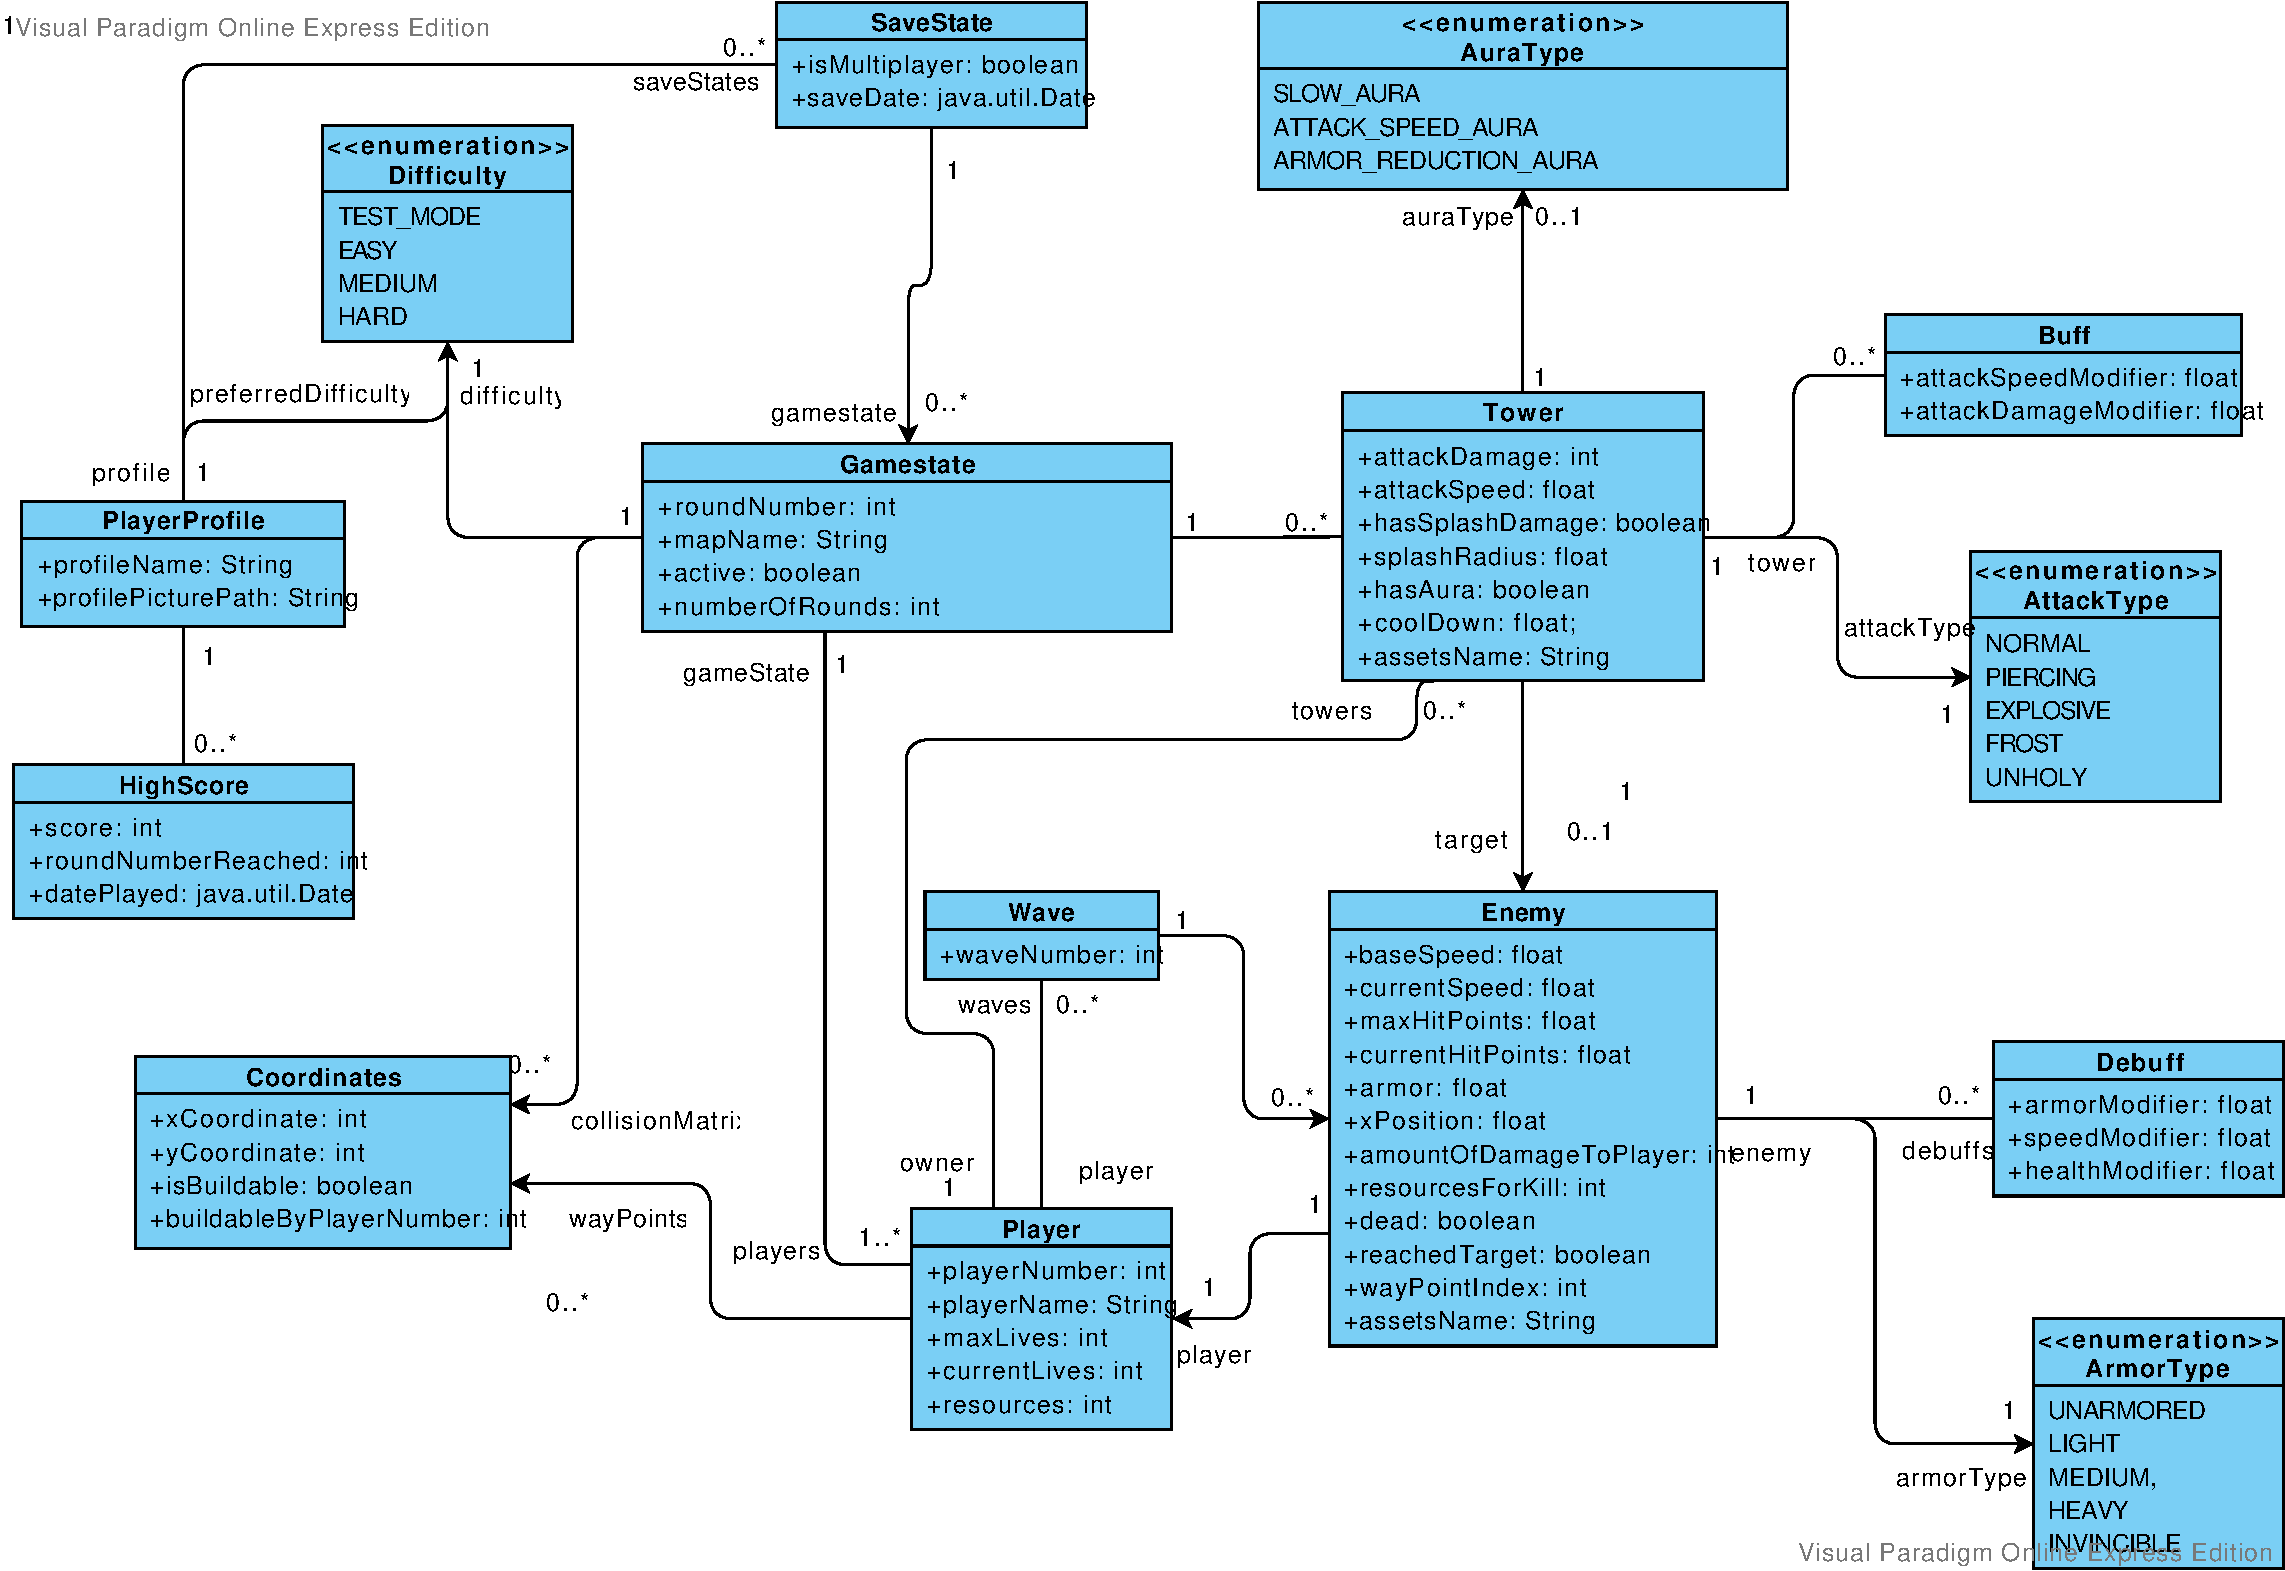
\includegraphics[width=\textwidth]{Bilder/Datenmodell.pdf}
    \caption{Darstellung unseres Datenmodells als UML-Klassendiagramm}
    \label{fig:Datensicht}
\end{figure}

Unser Datenmodell ist in \autoref{fig:Datensicht} dargestellt. Kern unseres Datenmodells ist der \texttt{GameState}, über den alle spielrelevanten Informationen abgerufen werden können. Dazu gehören die Spieler-Klasse, mit der Türme und Gegner-Wellen assoziiert sind. Türme und Gegner verfügen über zahlreiche Attribute, mit denen sich verschiedene Turm- und Gegner-Arten modellieren lassen. Aura-Arten, Angriffstypen, Rüstungstypen werden dabei ebenso wie die verschiedenen Schwierigkeitsgrade als \textit{Enumerables} modelliert. Über Spielprofile werden Informationen wie Highscores sowie Speicherstände gespeichert.

Die Darstellung in \autoref{fig:Datensicht} entspricht dabei auch der Abbildung auf die Datenbank. Die genaue Modellierung der Relationen sowie die Benennung der Tabellen und Verweise lässt sich die Annotationen in der Schnittstellenbeschreibung entnehmen.

\subsection{Konkretisiertes Transportmodell}
\label{subsec:datenmodell}

Wie in \autoref{fig:comPak} auf Seite \pageref{fig:comPak} dargestellt wird, nutzen wir für die Kommuniaktion zwischen Client und Server Request- und Response-Objekte, die mit den Operationen des GameControllers korrespondieren und beim Empfangen entsprechende Operationen des jeweiligen Controllers auslösen. Diese Funktionalität wird über passende Listener realisiert, die dem Server- beziehungsweise Client-Objekt aus der Kryonet-Bibliothek hinzufügt werden.


\clearpage

\section{Ausführungssicht}

\label{sec:ausfuehrung}

In \autoref{fig:GUI-Paket} ist unsere Software in der Ausführugssicht dargestellt. Wie sich \autoref{fig:GUI-Paket} entnehmen lässt, laufen auf beiden Ausführungssystemen zwei Prozesse parallel: Ein \texttt{GameClient}-Prozess, der die Funktionen aus der Paketsicht umsetzt, und ein Datenbank-Prozess, über den die Speicherung des GameState verwirklicht wird. Zwischen den beiden PCs findet ein Datenaustausch über TCP/IP statt. Das \texttt{Persistence}-Paket stellt die Schnittstelle vom Core-Modul zur Datenbank bereit.

\begin{figure}[H]
    \centering
    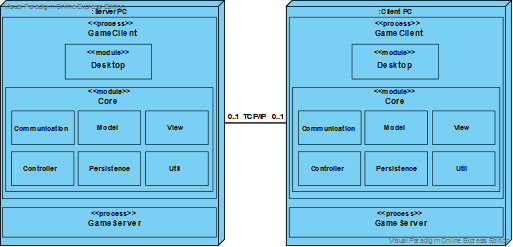
\includegraphics[width=\textwidth]{Bilder/ausfuehrungssicht.jpg}
    \caption{Ausführungssicht}
    \label{fig:GUI-Paket}
\end{figure}
%{\it
%Die Ausführungssicht beschreibt das Laufzeitverhalten. Hier
%werden die Laufzeitelemente aufgeführt und beschrieben, welche Module
%sie zur Ausführung bringen. Ein Modul kann von mehreren
%Laufzeitelementen zur Laufzeit verwendet werden. Die Ausführungssicht
%beschreibt darüber hinaus, welche Laufzeitelemente spezifisch
%miteinander kommunizieren. Zudem wird bei verteilten Systemen
%(z.\,B. Client-Server-Systeme) dargestellt, welche Module von welchen
%Prozessen auf welchen Rechnern ausgeführt werden.}

\clearpage

\section[Zusammenhänge zwischen Anwendungsfällen und Architektur]{Zusammenhänge zwischen Anwendungsfällen und Architektur\sectionmark{Zusammenhänge AF u. Architektur}}
\sectionmark{Zusammenhänge AF u. Architektur}
\label{sec:zusammenheange}

In diesem Abschnitt erläutern wir anhand von UML-Squenzdiagrammen, wie die einzelnen Elemente unserer Software bei deren Ausführung zusammenwirken. Hierzu betrachten wir die zwei wesentlichen Anwendungsfälle unserer Software: Das Starten und Spielen eines Single- sowie eines Multiplayer-Spiels, letzteres inklusive des Hostens einer Session als Server. %Diese Anwendungsfälle sind in \autoref{fig:usecases} als UML-Usecase-Diagramm dargestellt.

% \begin{figure}[H]
%     \centering
%     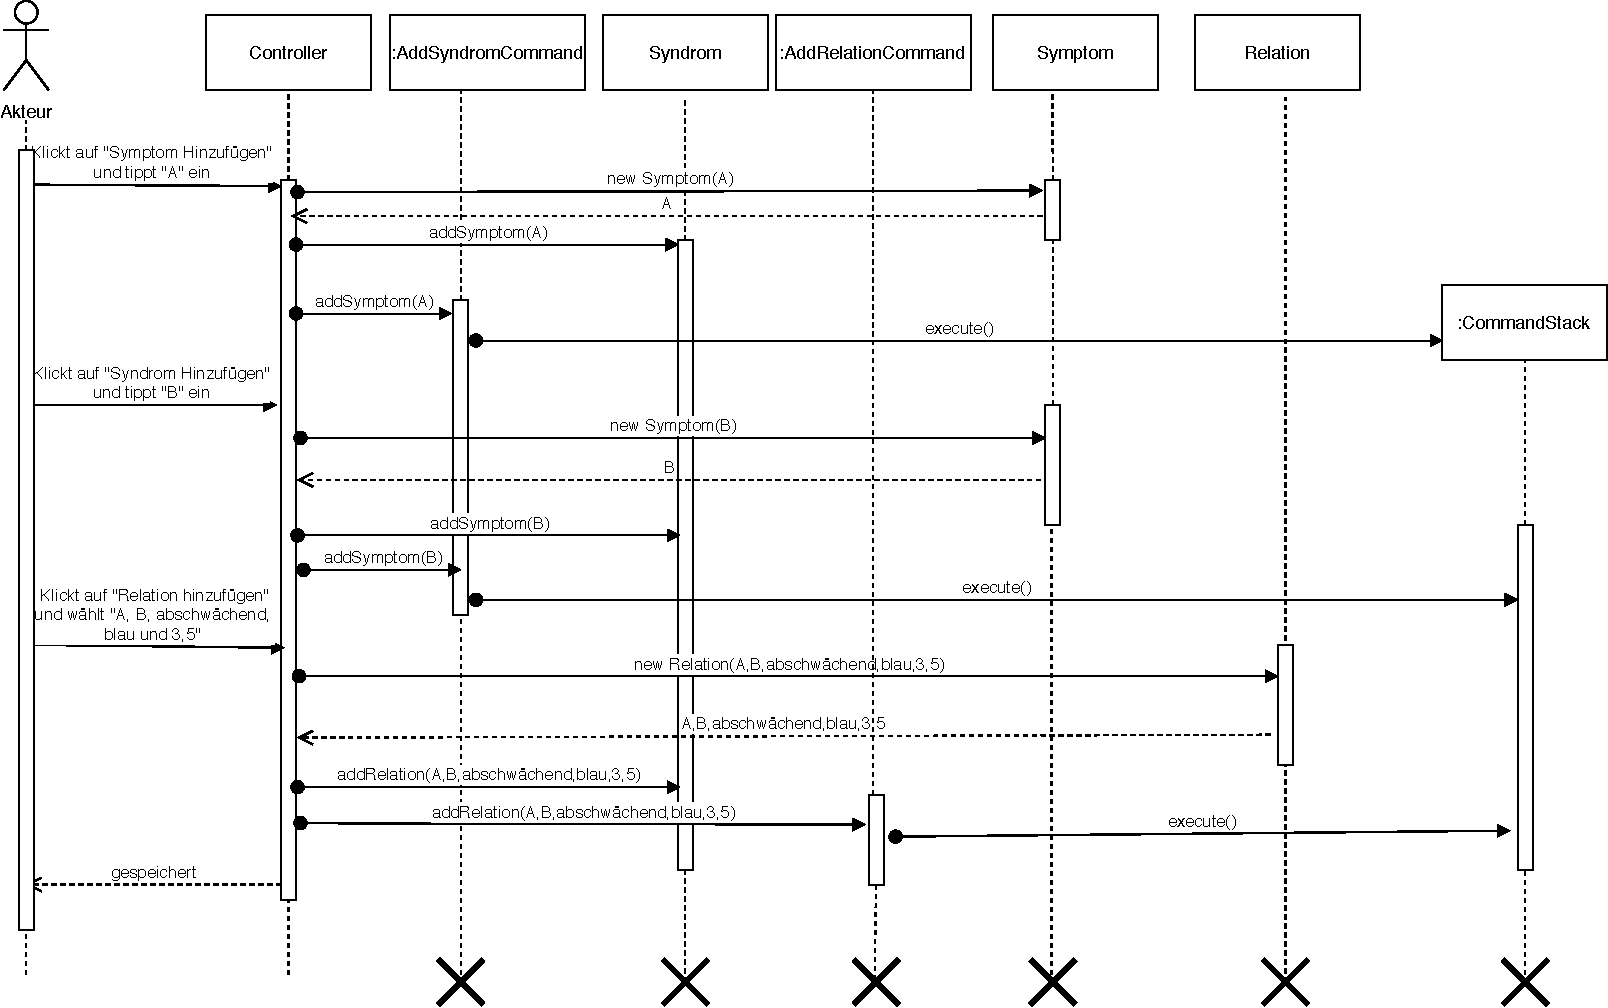
\includegraphics[width=\textwidth]{Bilder/SyndromansatzSWP.pdf}
%     \caption{UML-Anwendungsfall-Diagramm (noch durch ein tatsächliches Diagramm zu ersetzen)}
%     \label{fig:usecases}
% \end{figure}
% \clearpage

% \begin{landscape}

\subsection{Erstellen eines Verlangsamungs-Turms des Clientspielers}

\subsubsection{Beschreibung des Anwendungsfalls}

Ein Spieler möchte einen Verlangsamungs-Turm erstellen.Dazu klickt er an die entsprechende Stelle auf der Karte und wählt den gewünschten Turm aus. Das Geld wird dabei vom Konto des Spielers abgebucht und, falls genug vorhanden ist, der Turm plaziert. 

\subsubsection{Umsetzung in Exmatrikulator TD}

Die Umsetzung dieses Anwendungsfalls ist in \autoref{fig:SyndromansatzSWP} beschrieben. Zunächst wird vom GameLogicController des Clients uber den GameClient und GameServer auf den GameLogicController des Servers zugegriffen. Hier wird überprüft, ob der Spieler genug Geld hat (und dieses eventuell eingezogen) und ob die Position des Turms frei ist. Danach wird der Turm vom ServerGameLogicController erstellt und der GameClient wird Synchronisiert.

\begin{figure}[ht!]
    \centering
    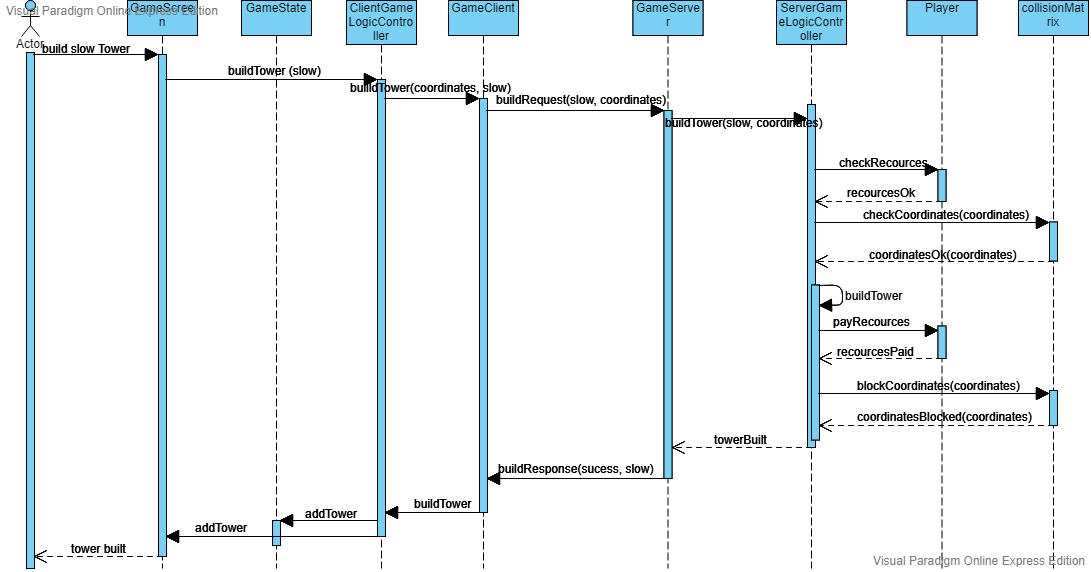
\includegraphics[width=\textwidth]{Bilder/sequence_build_slow_tower.png}
    \caption{Sequenzdiagramm 1}
    \label{fig:SyndromansatzSWP}
\end{figure}

% Hierfür klickt der Benutzer auf den Button \enquote{Symptom hinzufügen}, dann muss nur noch eine Bezeichnung für das Symptom vom Benutzer eingegeben werden. Anschließend wiederholt der Benutzer den Prozess, da er insgesamt zwei Symptome einfügen möchte. Nachdem es dem Benutzer gelungen ist, zwei Symptome einzufügen, möchte er die beiden Symptome mittels einer Relation verbinden. Dafür muss er auf den Button \enquote{Relation hinzufügen} klicken und dazu angeben, welche der beiden Symptome er verbinden möchte. Zudem muss er noch die Farbe und Stärke angeben und um welche Art von Relation es sich handelt. Im Anschluss wird das Dokument gespeichert.
\clearpage
% \end{landscape}



\subsection {Senden einer zusätzlichen Angriffswelle des ServerSpielers}

\subsubsection{Beschreibung des Anwendungsfalls}

Der Spieler möchte seinem Gegner das Leben schwer machen und schickt ihm einen zusätzlichen Gegner. Dazu wählt er  aus dem dafür vorgesehenen Drop-Down-Menü einen aus. Falls ihm genug Recourcen zur Verfügung stehen, wird dieser der nächsten Angriffswelle des Gegenspielers hinzugefügt.

\subsubsection{Umsetzung in Exmatrikulator TD}

Die Umsetzung dieses Anwendungsfalls ist in \autoref{fig:SyndromansatzSWP2} beschrieben.
Der GameLogicController des Servers prüft zunächst, ob der Spieler die benötigten Recourcen besitzt. Falls dem so ist, werden diese eingezogen und der Gegner über den Gamestate der Angriffswelle hinzugefügt. Außerdem wird der CLient wieder synchronisiert.

\begin{figure}[H]
    \centering
    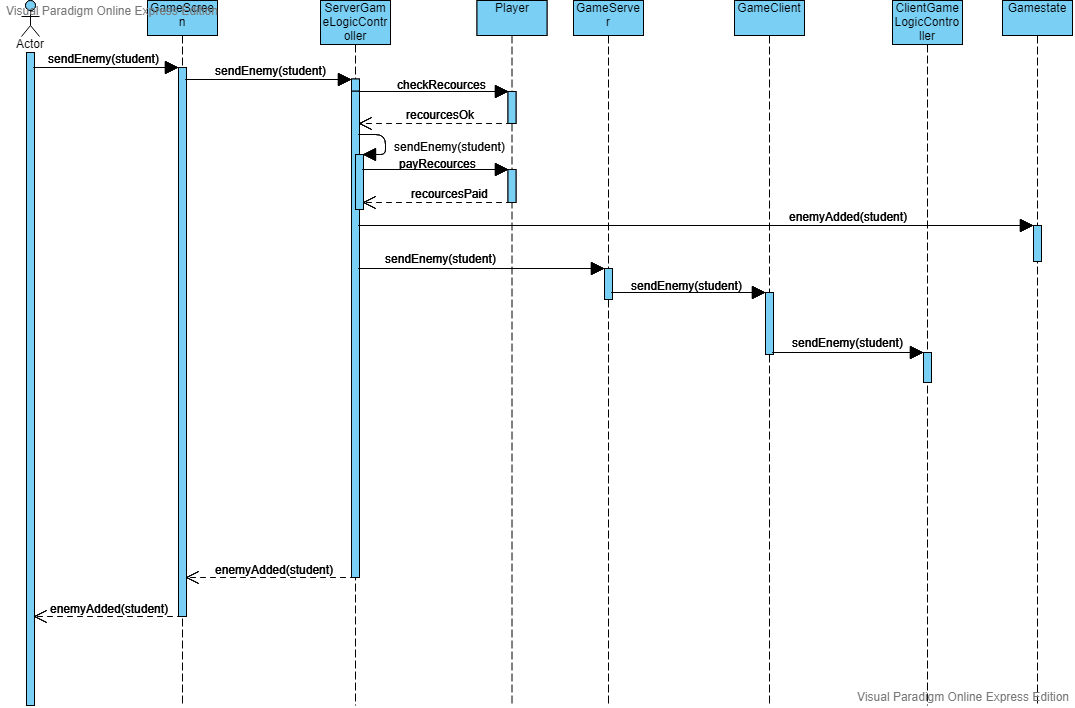
\includegraphics[width=\textwidth]{Bilder/sequence_send_wave.png}
    \caption{Sequenzdiagramm 2}
    \label{fig:SyndromansatzSWP2}
\end{figure}
\newpage


% {\it In diesem Abschnitt sollen Sequenzdiagramme mit Beschreibung(!)
%   für zwei bis drei von Euch ausgewählte
%     Anwendungsfälle
%   erstellt werden. Ein Sequenzdiagramm beschreibt den
%   Nachrichtenverkehr zwischen allen Modulen, die an der Realisierung
%   des Anwendungsfalles beteiligt sind.  Wählt die
%     Anwendungsfälle so, dass nach Möglichkeit alle Module Eures
%     entworfenen Systems in mindestens einem Sequenzdiagramm
%     vorkommen. Falls Euch das nicht gelingt, versucht möglichst viele
%     und die wichtigsten Module abzudecken. }

\section{Evolution}

\label{sec:evolution}

% {\it
%   Beschreibt in diesem Abschnitt, welche Änderungen Ihr
%   vornehmen müsst, wenn sich Anforderungen oder Rahmenbedingungen
%   ändern. Insbesondere würden hierbei die in der
%   Anforderungsspezifikation unter "`Ausblick"' genannten
%   Punkte behandelt werden.}

% \subsection{Mobilanwendungen}

In diesem Abschnitt wird beschrieben, welche Änderungen an der Architektur vorzunehmen sind, wenn sich eine Reihe von Anforderungen ändern bzw. zu den bereits berücksichtigten hinzukommen. In diesem Rahmen zeigen wir weiterhin auf, welche Entwicklungspotentiale unser Spiel hat.

\subsection{Bereitstellung für als Android-, iOS- und HTML5-Version}

Durch Nuzung von LibGdx lässt sich unser Spiel relativ leicht auf andere Plattformen portieren: Ein jeweiliges plattformspezifisches Modul (in dieser Archtitekturbeschreibung das Modul \enquote{Desktop}) greift im Wesentlichen auf den Inhalt der Core-Komponente zu und setzt das dort implementierte Spiel mit plattformspezifisch um.

Die bestehende Architektur sollte sich folglich relativ leicht um weitere Plattformen, namentlich Android, iOS und HTML5, erweitern lassen, wobei hierbei auf die Spezifika der Zielplattformen (wie etwa die unterschiedlichen Bildschirmgrößen) Rücksicht genommen werden muss. Da die Kryonet-Bibliothek jedoch nicht mit iOS kompatibel ist, muss für diese Plattform auf eine andere Netzwerk-Bibliothek zurückgegriffen werden. 

Gerade bei der browserbasierten HTML5-Version sollte zudem eine andere Client-Server-Architektur diskutiert werden, die die Funktionalität des Servers auf einen dezidierten Server verlagert. 

\subsection{Mehrsprachigkeit der GUI}
Um nicht nur deutschsprachigen Nutzern den Spielspa{\ss} zu erm"oglichen, sollen nachtr"aglich Sprachpakete installierbar sein, sodass die grafische Oberfläche in der gewünschten Sprache erscheint. 
Hierzu müsste eine Schnittstelle geschaffen werden, die das Einlesen von Dateien im geeigneten Format erlaubt. Diese könnten anschließend z. B. der eingebetteten Datenbank gespeichert werden, was eine Erweiterung des Persistance-Paketes bedeuten würde. Bei Wechsel der Sprache könnten die Strings für die Felder in der GUI dann für einen schnelleren Abruf entweder in den jeweiligen Menü-Elementen selbst oder in einer Datenstruktur wie einer  Hashmap gespeichert werden.

\subsection{Bereitstellung eines Map-Editors}
Da mit der Auslieferung nur die hartkodierten Maps zur Verf"ugung stehen, soll es m"oglich seien nachtr"aglich Maps selbst zu erstellen und mit Mitspielern zu teilen. Dies kann z.B. mittels dem \begin{it}Tiled Map Editor\end{it} geschehen, womit bereits die Maps, welche mit der Anwendung ausgeliefert werden, kreiert wurden. Dementsprechend m"usste nur noch eine Schnittstelle innerhalb der Anwendung geschaffen werden, welche das nachtr"agliche Einbinden von Maps erlaubt.

% \begin{figure}[H]
%     \centering
%     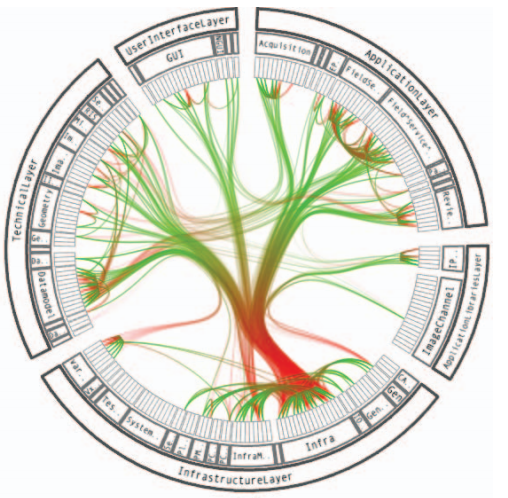
\includegraphics[width=.5\textwidth]{Bilder/Kantenbuendelung.png}
%     \caption{Beispiel für eine kreisförmige Anordnung von Knoten mit gebündelten Kanten (Quelle: Danny Holten \cite{Holten2006}).}
%     \label{fig:kantenbuendelung}
% \end{figure}

\end{document}